\documentclass[final]{clv2025-revised}

\jvol{vv}
\jnum{nn}
\jyear{2025}
%There is no need for the authors to change the above.

%\dochead{An Example of Document Head} 
% Possible options: Long Paper, Short Paper, Survey, Survey Proposal, Position Paper, Last Words, Book Review, Dissertation Award, Lifetime Achievement Award, Squibs and Discussions, Featured Article

\pageonefooter{Action editor: \{action editor name\}. Submission received: DD Month YYYY; revised version received: DD Month YYYY; accepted for publication: DD Month YYYY.}
% To be filled when the paper is accepted. The editorial office will share the relevant information with the authors. Example: Action Editor: Wei Lu. Submission received: 10 February 2023; revised version received: 30 May 2023; accepted for publication: 15 June 2023.

\usepackage{amsmath}
\usepackage{booktabs}
\usepackage{tabularx}

\runningtitle{Layer Cake}
\runningauthor{Worth \& Cardei}

\begin{document}

\title{Layer Cake: On Language Representation and Compute Characteristics in Text Classification}

\author{Peter J Worth Jr.\thanks{Corresponding author}, Ionut Cardei}

\affilblock{
    \affil{Florida Atlantic University, Department of Electrical Engineering and Computer Science, Boca Raton, FL\\\quad \email{pworth2022@fau.edu}}
    \affil{Florida Atlantic University, Department of Electrical Engineering and Computer Science, Boca Raton, FL\\\quad \email{icardei@fau.edu}}
}

\maketitle

\begin{abstract}
Since transformer-based language models were introduced in 2017, they have been shown to be extraordinarily effective across a variety of NLP tasks including but not limited to language generation. The introduction and widespread adoption of these LLMs, which encode extremely high-dimensional semantic spaces, comes at a significant cost in terms of system and computational resource requirements, requirements that have reshaped the entire chip (GPU) and data center industry as hardware, cloud, and infrastructure providers try to keep up with the demand. This has motivated the research community to develop a variety of design strategies that optimize the use of these resources; however, computational requirements continue to grow in proportion to model size and complexity. With this study, we introduce a framework called Layer Cake for the precise measurement of the relative computational resource requirements necessary for text classification using a variety of classifiers from across the Machine Learning (ML) and Deep Learning (DL) landscape, leveraging different language model families and focusing on the forms of language representation used in different test scenarios. We find that while LLMs do yield the best results across classifiers on average, these improvements come at a significant computational overhead. For example, from a Macro-F1 score perspective, LLM-based classifiers outperform their static embedding language model counterparts (Word2Vec, FastText \& GloVe), even when encapsulated in DL architectures such as Convolutional Neural Networks or Long-Short-Term Networks by 8.87\% on average, and perform 12.73\% better than ML classifiers such as Support Vector Machines and Logistic Regression models. However, this uptick in model performance comes at a computational overhead cost of 4398.07\% compared to the GPU requirements of static word embedding DL classifiers, and a 4126.02\% increase in computation time relative to ML classifiers, the latter of which are CPU, rather than GPU, bound.
\end{abstract}


\keywords{Text Classification, Large Language Models, LLMs, Natural Language Processing, NLP, Language Representation, Word Embeddings, Vector Space Models, Semantic Spaces, Artificial Intelligence, AI, Computational Linguistics}

\section{Introduction}

Since the introduction of ChatGPT in Nov 2022, we have been in the midst of the most rapid and broad reaching technological transformation since the advent of broadband technology and the development of the Internet which has ushered in the Digital Age, one of the foundational requisite components of the AI revolution, for without the mass digitization of text and language over the last few decades, there would be nothing to train these AI models with in fact. One startling fact of the broad reach of these tools, and of Chat GPT in particular is that as of May 2025, it was estimated that ChatGPT had nearly 800 million active weekly users and over 122 million active daily users.\footnote{Source: https://www.demandsage.com/chatgpt-statistics/}. And while there are many different tools, capabilities and underlying technologies that underpin this AI revolution, one of the primary drivers is the development of software applications that can generate coherent and powerful analytical, rational natural language responses to natural language inputs, or prompts as they are more commonly called now - natural language generation (NLG) tools as they are called.

Language models are a technological advancement first introduced in 2012 \cite{mikolov} which looked to provide a more effective, and efficient, means of representing language (i.e. \textit{word embeddings}) which in turn led to the development of what have come to be known ad \textit{large language models}\textit, or LLMs, which leverage transformer-based architectures \cite{vaswani} (introduced in 2017) along with multi-head attention mechanisms in a deep learning (DL) context to construct language models that can both represent the generic meaning of words, subwords or tokens based upon a pre-trained corpus of text that the model is trained on, as well as generate representations of tokens, words and subwords that reflect the specific context within which the underlying word, subword or token is a found in a given text or document within a given corpus, opening up a whole new set of NLG and reasoning capabilities that are fueling the adoption of this transformative technology into almost every industry vertical and every part of the technology stack. Furthermore, these language models can be adapted, or \textit{fine-tuned}, for all sorts of different NLP tasks such as text classification, text summarization, sentiment analysis, etc., each of which has broad application to fields ranging from technology, to finance, to bio-chemistry, to genomics, to cyber security.

LLMs are \textit{context-aware} language models which are pre-trained on vast amounts of digital text, or corpora, and are constructed using deep learning (DL) techniques and neural networks that have been the subject of research in the Computer Science, AI and Natural Language Processing (NLP) community since at least the 1970s, but the effectiveness of these approaches has been greatly enhanced over the last few years due to revolutionary advancements in software architecture yes, but also from advancements in hardware which has been designed specifically to support the type of operations, and scale, necessary to build LLMs which underpin this rapid advancement of AI technology. We speak here of specialized processing units manufactured by companies like NVIDIA, Intel, AMD and Google (among others) called GPUs (graphical processing units), or TPUs (tensor processor units), which differ from their CPU counterparts because they are designed and optimized specifically for the type of massively parallelized linear algebraic operations which are fundamental to the training, and use, of LLMs. This hardware in turn relies on specialized software which supports the distributed processing and computation of these matrices, or \textit{tensors}, across massive server farms which connect hundreds, and sometimes thousands, of these specialized processing units.\footnote{CUDA for example, produced by NVIDIA in 2006 which is arguably the most widely adopted software which handles the synchronization, distribution and collation of the all of these matrices and tensors across these distributed server farms of GPUs.} This wave of technological transformation underpinned by the power and availability of LLMs is unprecedented - in terms of the amount of research that has been produced in this area over the last several years \cite{naveed2024comprehensiveoverviewlargelanguage} \cite{fan2023bibliometricreviewlargelanguage}, in terms of the number of models that have been produced and now available for public consumption which is now measured in the thousands \footnote{As of June 2004 the number of available LLMs on Hugging Face was estimated to be over 700,000. See https://www.marktechpost.com/2024/06/15/with-700000-large-language-models-llms-on-hugging-face-already-where-is-the-future-of-artificial-intelligence-ai-headed/}, and in terms of the demand for infrastructure to support the development, training, hosting, and use of these models.\footnote{The value of the Data Center market for 2024 was 242.72 billion and by 2032 is estimated to be at 584.86 billion. Source: https://www.fortunebusinessinsights.com/data-center-market-109851}. There has also been significant research done on the socio-economic impacts of this rapid advancement in AI \cite{10.1093/pnasnexus/pgae191} \cite{El-Farr24}, and no doubt this is just the beginning.

Architecturally speaking, each of these LLMs comes with a pre-computed set of (static) embeddings for each token in its dictionary which identify, and more precisely geometrically locate, each token in the underlying feature space, what we refer to as the underlying \textit{semantic space} \cite{worth}. These static embeddings are computed during pre-training based upon the specific training techniques used by the underlying LLM and based off of some fundamental linguistic theories (more on this below). Some of the most common methods of training include \textit{next token prediction}\footnote{Next token prediction based LLMs are called \textit{causal} language models due to the determinative nature of the underlying algorithm.} which is used for example by the GPT family of models built by OpenAI \cite{radford2019language}, and \textit{masking} which is used by the BERT \cite{devlin-etal-2019-bert} and RoBERTa \cite{liu2019roberta} based language model families models. All of these transformer-based LLMs however ultimately leverage these static, pre-trained token embeddings for generating dynamic, context-aware forms of language representation during inference time, which facilitate the generation of a much more nuanced and specific representation of (natural) language, or text, than their static word embedding language model predecessors and provide the architectural foundations from which the LLMs derive their interpretative power. 

All LLMs fundamentally use the same basic approach to how they represent language, they simply differ in terms of a) the token dictionary which underpins the model which defines the basic granularity, or set of dimensions or features, which define the underlying semantic space of the model, and b) the algorithm used to compute these static pre-trained token embedding vectors which is characteristic of the underlying LLM or family of LLMs. Each LLM therefore can be understood as consisting of \textit{both} a set of pre-computed, static tokens which are represented by a vector of real numbers that is the result of model pre-training that serves to define the basic lexicon, or the underlying semantic space, of the language model in question, \textit{and} the capability to generate context-sensitive token embeddings from the static pre-trained token embeddings, in conjunction with positional encoding information and multi-headed attention masking features which are fundamental to transformer-based language models, which facilitate much more powerful interpretive capabilities of these LLMs which have transformed the AI and technological landscape over the past few years. This is the basic architecture that was introduced in 2017 in the seminal "Attention is all you need" paper \cite{vaswani} except described from a semantic perspective, and it is hard to exaggerate the profound effect that these technological advancements have already had on the global technology and socio-economic landscape with more to come no doubt.

One of the areas where these LLMs have been found to be effective is \textit{text classification}, the core focus of the research in this work and one of the core NLP problems that has been well studied for decades and as such provides a good test bed to analyze the extent to which LLMs can improve performance of text classifiers and the cost, in terms of training time and computational requirements (number of GPUs or CPUs, amount of memory, etc.), incurred to achieve these performance gains. Traditionally, the problem of text classification has been approached through feature-engineered statistical models, falling under the rubric of Machine Learning (ML) which primarily include Naive Bayes approaches \cite{mccallum1998comparison}, Logistic Regression models, \cite{genkin01082007}, and Support Vector Machines \cite{joachims1998text}. The emergence of deep neural architectures and more powerful processors designed specifically for ML and AI type computations facilitated the advance of word embedding language models such as Word2Vec \cite{mikolov}, GloVe \cite{pennington}, and FastText \cite{articleboja} which were then used in DL models to push the boundaries for many NLP tasks, text classification being no exception \cite{zhang2015character} \cite{yoon2014convolutional} \cite{hochreiterlong}. Yet it was the introduction of transformer architecture in 2017 \cite{vaswani} followed shortly thereafter by the introduction of BERT \cite{devlin-etal-2019-bert} which demonstrated how powerful LLMs could be in establishing new benchmarks for NLG and NLP solves. The effectiveness of LLMs in this context demonstrated how powerful the combination of linguistics, deep learning, pretraining, attention masking and transformers, which underpinned the construction of vast, granular, semantic spaces which could be effectively navigated, searched basically, via the use of natural language prompts that could be transformed into token embeddings that can be used to generate very precise, and quite profound results across the NLP and AI landscape - capabilities which were predicated on  more advanced system and compute resources from which these spaces could be both constructed (model construction and pretraining) and searched (inference). 

Despite these advances, the computational cost associated with training as well as fine-tuning LLMs remains a pressing concern, driving a whole field of research in and of itself, much of which is grouped under the name of \textit{parameter-efficient finetuning} (PEFT), which includes a vast array of sophisticated techniques to adapt LLMs, i.e. \textit{finetune}, to specific tasks without retraining the entire model, i.e. recomputing all of the model weights. Some of the most influential of these methods include adapter tuning \cite{pmlr-v97-houlsby19a}, prefix tuning \cite{li2021prefixtuningoptimizingcontinuousprompts}, low ranked adaptation (LoRA) \cite{hu2021loralowrankadaptationlarge}, and variants of LoRA such as quantized low-rank adaptation (QLoRA) \cite{dettmers2023qloraefficientfinetuningquantized}, Adaptive Budget Allocation for Parameter-Efficient Fine-Tuning (AdaLoRA) \cite{zhang2023adaloraadaptivebudgetallocation} as well as related optimization techniques using LoRA like approaches such as S-LoRA \cite{sheng2024sloraservingthousandsconcurrent} or SC-LoRA \cite{luo2025sclorabalancingefficientfinetuning}. However, these studies focus on comparative performance improvements gains for LLM fine-tuning without a detailed analysis of the underlying computational resource requirements necessary for a given model type for a give problem, leaving a significant blind spot for both researchers and practitioners in the field when trying to determine which approaches are best for a given problem within the context of specific economic constraints. This gap in the research is becoming more and more problematic as the NLP community pushes toward democratizing, open sourcing mostly, access to larger and more powerful (language) models, models which are so large that they have to be spread out across GPU farms in order to be constructed (trained) and maintained (kept up to date), developments which are putting increased pressure on access to advanced, state of the art computational resources (high end GPUs effectively) in order to reproduce many of the state of the art results which are driving the field forward.

In this work, we look to try and address this blind spot, at least partially, by focusing on one specific NLP problem that is representative of the domain at large, and conducting a comprehensive, systematic evaluation of approaches to the problem which span the ML, DL and LLM landscape using standard approaches to model adaption for the task at hand (finetuning) and leveraging industry standard benchmarks and metrics to measure and compare results which include data on the requisite computational and system requirements of each of the approaches. The platform that we built to support this testing, which also includes analytics capabilities, we call \textit{Layer Cake}, and it is based off of research and code produced in 2021 which looked at the effect of Word-Class Embeddings (WCEs) on classifier performance \cite{moreo2021}. In this work however, we look at the problem not just from a classifier perspective, but also from a language model and \textit{language representation} perspective as well so that we can see which forms of language representation, intrinsic to different language models, work best in which context \textit{and} produce data that helps us understand what the true cost, in terms of computational resource requirements, is for each of the different approaches to the problem. To this end we report results of each of the classifiers and language model variations we test in Layer Cake not just using the standard NLP metrics such as accuracy, macro-F1 and micro-F1, but we also report on, and analyze, model training times and underlying system resources used for each of the tests. Furthermore, as an additional contribution to the research community, we open source Layer Cake so that researchers and practitioners alike can both reproduce the results herein, as well as extend the platform further into the LLM landscape and/or into different aspects of NLP beyond text classification.\footnote{https://github.com/pworth1971/layer-cake} By shedding light on both the efficacy and expense of current NLP architectures, this study offers a performance-cost roadmap for more sustainable, scalable, and context-aware deployment of classification systems. 


\subsection{Supported Datasets}

The datasets used in Layer Cake span multiple domains, including news, academic publishing, medical research, and reviews. We evaluate datasets across a range of subject areas and sample from both single-label and multi-label datasets. This diversity allows for comprehensive benchmarking across different modeling designs, forms of language representation and datasets.

\begin{itemize}
    \item \textbf{Reuters-21578} \cite{lewis1987reuters}: A multi-label dataset containing 21,578 news documents across 115 categories. Although class imbalance is significant, it remains a standard benchmark for multi-label text classification research.
    
    \item \textbf{BBC News} \cite{greene}: A single-label dataset of 2,225 news articles categorized into five balanced topics: business, entertainment, politics, sport, and tech.
    
    \item \textbf{RCV1-V2} \cite{lewis2004}: A large-scale multi-label dataset with over 800,000 Reuters newswire stories spanning 103 overlapping categories, ideal for evaluating models on complex, real-world data.
    
    \item \textbf{20 Newsgroups} \cite{LANG1995331}: A well-known single-label dataset containing approximately 20,000 documents across 20 categories, widely used for benchmarking text classification algorithms.
    
    \item \textbf{arXiv} \cite{sinha}: A multi-label dataset of research papers from the arXiv repository, covering 58 scientific disciplines. It tests model robustness on technical, domain-specific vocabulary.
    
    \item \textbf{arXiv protoformer} \cite{farhangi}: A simplified, single-label subset of the arXiv dataset focused on the 10 most common scientific categories, frequently used for prototype-based model experiments.
    
    \item \textbf{OHSUMED} \cite{sanderson}: A multi-label dataset comprising medical abstracts labeled with 23 MeSH (Medical Subject Headings) classes, presenting challenges due to its highly specialized vocabulary.
    
    \item \textbf{IMDB} \cite{maas}: A binary classification dataset of movie reviews labeled as positive or negative, balanced across training and test splits. The significant variance in review lengths adds additional modeling complexity.
\end{itemize}

A summary table of the different datasets we use with Layer Cake and their basic characteristics is provided below in Table 1 below.

\sloppy
\begin{table}[h!]
\centering
\caption{Summary of datasets used in Layer Cake and their basic characteristics.}
\label{tab1}
\scriptsize
\begin{tabularx}{\textwidth}{l c c c X}
\toprule
\textbf{Dataset} & \textbf{Type} & \textbf{Classes} & \textbf{Size} & \textbf{Characteristics} \\
\midrule
Reuters-21578 & multi-label & 115 & 64 MB & News articles, imbalanced class distribution. \\
BBC News & single-label & 5 & 6.7 MB & Balanced topics from BBC news. \\
arXiv & multi-label & 58 & 5.5 GB & Research papers, overlapping categories. \\
arXiv Protoformer & single-label & 10 & 147 MB & Simplified version of arXiv for single-label tasks. \\
IMDB & single-label & 2 & 694 MB & Movie reviews, sentiment analysis. \\
OHSUMED & multi-label & 23 & 387 MB & Medical abstracts, domain-specific. \\
RCV1-v2 & multi-label & 101 & 7.4 GB & Large-scale news corpus, hierarchical topics. \\
20 Newsgroups & single-label & 20 & 15 MB & Newsgroup articles, balanced and diverse topics. \\
\bottomrule
\end{tabularx}
\end{table}


\subsection{Supported Language Models}

Layer Cake supports a wide array of language models, enabling a comparison of different forms of language representation and an analysis of how model design and training objectives affect classifier effectiveness. While Layer Cake supports various evaluation measures, we primarily focus on Macro-F1 and Micro-F1 scores, following \cite{moreo2021}, as they provide holistic views of classifier performance. 

For static, word-based embeddings, we evaluate GloVe, Word2Vec, and FastText models. These embeddings were trained on the Common Crawl dataset, a large-scale, multilingual web corpus consisting of over 600 billion tokens.\footnote{Source: https://commoncrawl.org/} The GloVe model \cite{pennington} we use is glove.840B.300d.txt which captures global co-occurrence statistics across a large corpus, providing 300-dimensional embeddings. The Word2Vec model \cite{mikolov}, GoogleNews-vectors-negative300.bin, was trained on Google News data using CBOW and skip-gram methods with negative sampling for efficient learning, and the FastText \cite{articleboja} model we use is crawl-300d-2M.vec.bin, which extends Word2Vec by incorporating subword information, enabling generalization to out-of-vocabulary words.

\begin{table}[h!]
\centering
\scriptsize
\caption{Layer Cake Supported Language Models}
\renewcommand{\arraystretch}{1.1}
\begin{tabular}{@{}p{1.2cm} p{2cm} p{1.8cm} p{1.7cm} p{1.2cm} p{2.2cm} p{0.7cm}@{}}
\toprule
\textbf{Family} & \textbf{Model Name} & \textbf{Training} & \textbf{Architecture} & \textbf{\# Params} & \textbf{Data Source} & \textbf{Dim} \\
\midrule
GloVe & glove.840B.300d & Co-occurrence & Embedding & 2.2M & Common Crawl & 300 \\
Word2Vec & GoogleNews-300 & Skip-gram & Embedding & 3M & Google News & 300 \\
FastText & crawl-300d-2M & Skip-gram & Embed+Subword & 2M & Common Crawl & 300 \\
\midrule
BERT & bert-base-cased & MLM+NSP & Encoder & 110M & Wiki+BooksCorpus & 768 \\
RoBERTa & roberta-base & MLM & Encoder & 125M & WebText+CCNews & 768 \\
DistilBERT & distilbert-base & MLM Distill & Encoder & 66M & Same as BERT & 768 \\
XLNet & xlnet-base-cased & Permutation LM & Autoregressive & 110M & Wiki+Books+ClueWeb & 768 \\
GPT-2 & gpt2 & Next Token & Decoder & 117M & WebText & 768 \\
Llama & Llama-3.2-1B & Next Token & Decoder & 1.2B & CCNet+Books & 2048 \\
DeepSeek & DeepSeek-R1-1.5B & Next Token Distill & Decoder & 1.5B & Web+Academic+Code & 1536 \\
\bottomrule
\end{tabular}
\end{table}

The supported transformer-based language models we support, models we refer to as 'context-aware' given their support for attention masking and positional encoding information, include language models from the BERT, RoBERTa, DistilBERT (distilbert-base-cased), XLNet, GPT-2, Llama, and DeepSeek families (see Table 2 above for details). BERT \cite{devlin-etal-2019-bert} and RoBERTa \cite{liu2019roberta} are pretrained using masked language modeling (MLM), with BERT also using next sentence prediction (NSP). RoBERTa modifies BERT by removing NSP and adjusting pretraining strategies to improve generalization. DistilBERT \cite{sanh2020distilbert}, based on BERT, uses knowledge distillation \cite{hinton2015distilling} to create a lighter, faster model while retaining most of BERT's performance. XLNet \cite{yang2019xlnet} builds on Transformer-XL \cite{dai2019transformer} and introduces permutation-based training to capture bidirectional context without masking, blending ideas from both encoder and autoregressive architectures and GPT-2 \cite{radford2019language} is an autoregressive, decoder-only model trained to predict the next token in a sequence, enabling strong generative capabilities. It serves as a contrast to masked transformer models like BERT. 

Llama, introduced by Meta in 2023 \cite{touvron2023llama}, is a decoder-only transformer, an autoregressively trained LLM optimized for efficient scaling and multilingual generation tasks. These models are pretrained on a broad corpus of texts across multiple languages and are also tuned using supervised fine-tuning (SFT) and reinforcement learning with human feedback (RLHF) methods. We also include one of the smaller DeepSeek models in our study. This family of transformer-based models are known for their efficiency and reasoning capabilities, and have achieved strong results on a variety of complex NLP tasks \cite{articlebi, guo2025deepseek}. DeepSeek models utilize reinforcement learning without preliminary SFT \cite{ouyang2022training} and incorporate chain-of-thought reasoning strategies \cite{articlewei}. In our evaluation, we also include a distilled DeepSeek model based on techniques similar to those used for optimizing Qwen models \cite{articlebai, hinton2015distilling}.

Detailed specifications around the language models we used for this research, supported by Layer Cake, can be found in Table 2 above.

\subsection{Supported Classifiers}

The Layer Cake architecture for text classification integrates three distinct classifier modules, each designed to leverage different language modeling approaches and classifier types. This modular design facilitates comprehensive evaluation and comparison across traditional machine learning methods, static language model embeddings, and advanced transformer-based architectures.

\textbf{Machine Learning Classifiers (ML):} This module includes classical ML algorithms frequently used in text classification tasks: Support Vector Machines (SVM) \cite{joachims1998text}, Logistic Regression (LR) \cite{genkin01082007}, and Naive Bayes (NB) \cite{mccallum1998comparison}. These classifiers operate directly on vectorized text features, typically using bag-of-words representations such as TF-IDF or Count vectors, and serve as robust baseline methods due to their computational efficiency and interpretability. We also add a variety of feature reduction techniques and language representation forms to illustrate the flexibility, and relative performance, of different approaches to representing the text in these classifiers. All of these classifiers leverage the Python scikit-learn libraries\footnote{https://scikit-learn.org/stable/} and (primarily) rely on the CPU for processing.

\textbf{Static Language Model Classifiers (Static LM):} The second module employs neural network-based classifiers, originally presented in \cite{moreo2021}, which are designed to leverage pre-trained static word embedding language models such as Word2Vec \cite{mikolov}, GloVe \cite{pennington} and FastText \cite{articleboja} models. We include three different types of neural classifiers in this module, each of which is constructed using Python PyTorch libraries\footnote{https://pytorch.org/}: Convolutional Neural Networks (CNN) \cite{yoon2014convolutional}, Attention-based models (ATTN) \cite{liuguo2019bidirectional}, and Long Short-Term Memory networks (LSTM) \cite{hochreiterlong}. The static embeddings provide fixed semantic representations of words (and subwords in the case of FastText), capturing general linguistic regularities without adapting dynamically to the context, hence we refer to these as 'static' classifiers and language models throughout.

\textbf{Transformer-based Classifiers:} The final module incorporates transformer-based classifiers using the Hugging Face Transformers library\footnote{https://huggingface.co/docs/transformers/en/index}. We support two primary architectures: the standard Sequence Classification model, which utilizes pretrained transformer models such as BERT \cite{devlin-etal-2019-bert}, RoBERTa \cite{liu2019roberta}, DistilBERT \cite{sanh2020distilbert}, XLNet \cite{yang2019xlnet}, GPT-2 \cite{radford2019language}, Llama \cite{touvron2023llama}, and DeepSeek \cite{guo2025deepseek}; and a transformer-based CNN architecture, integrating transformers' context-aware embeddings with convolutional layers to enhance feature extraction and drive classification performance. Our approach with the transformer-based classifiers is to fine-tune the model against each of the  datasets, leveraging the classification head that sits at the tail end of the neural network and performs the actual classification after the dataset is encoded with the transformer specific embeddings. Details on how this done, and the specifics of the neural architecture, can be found in the Layer Cake Design section below. 

Figure 1 summarizes these different Layer Cake modules and their corresponding classifiers. This structured classification setup provides a versatile and systematic framework for evaluating classifier performance and exploring how different linguistic representations influence classification outcomes.

\begin{figure}[h!]
  \centering
  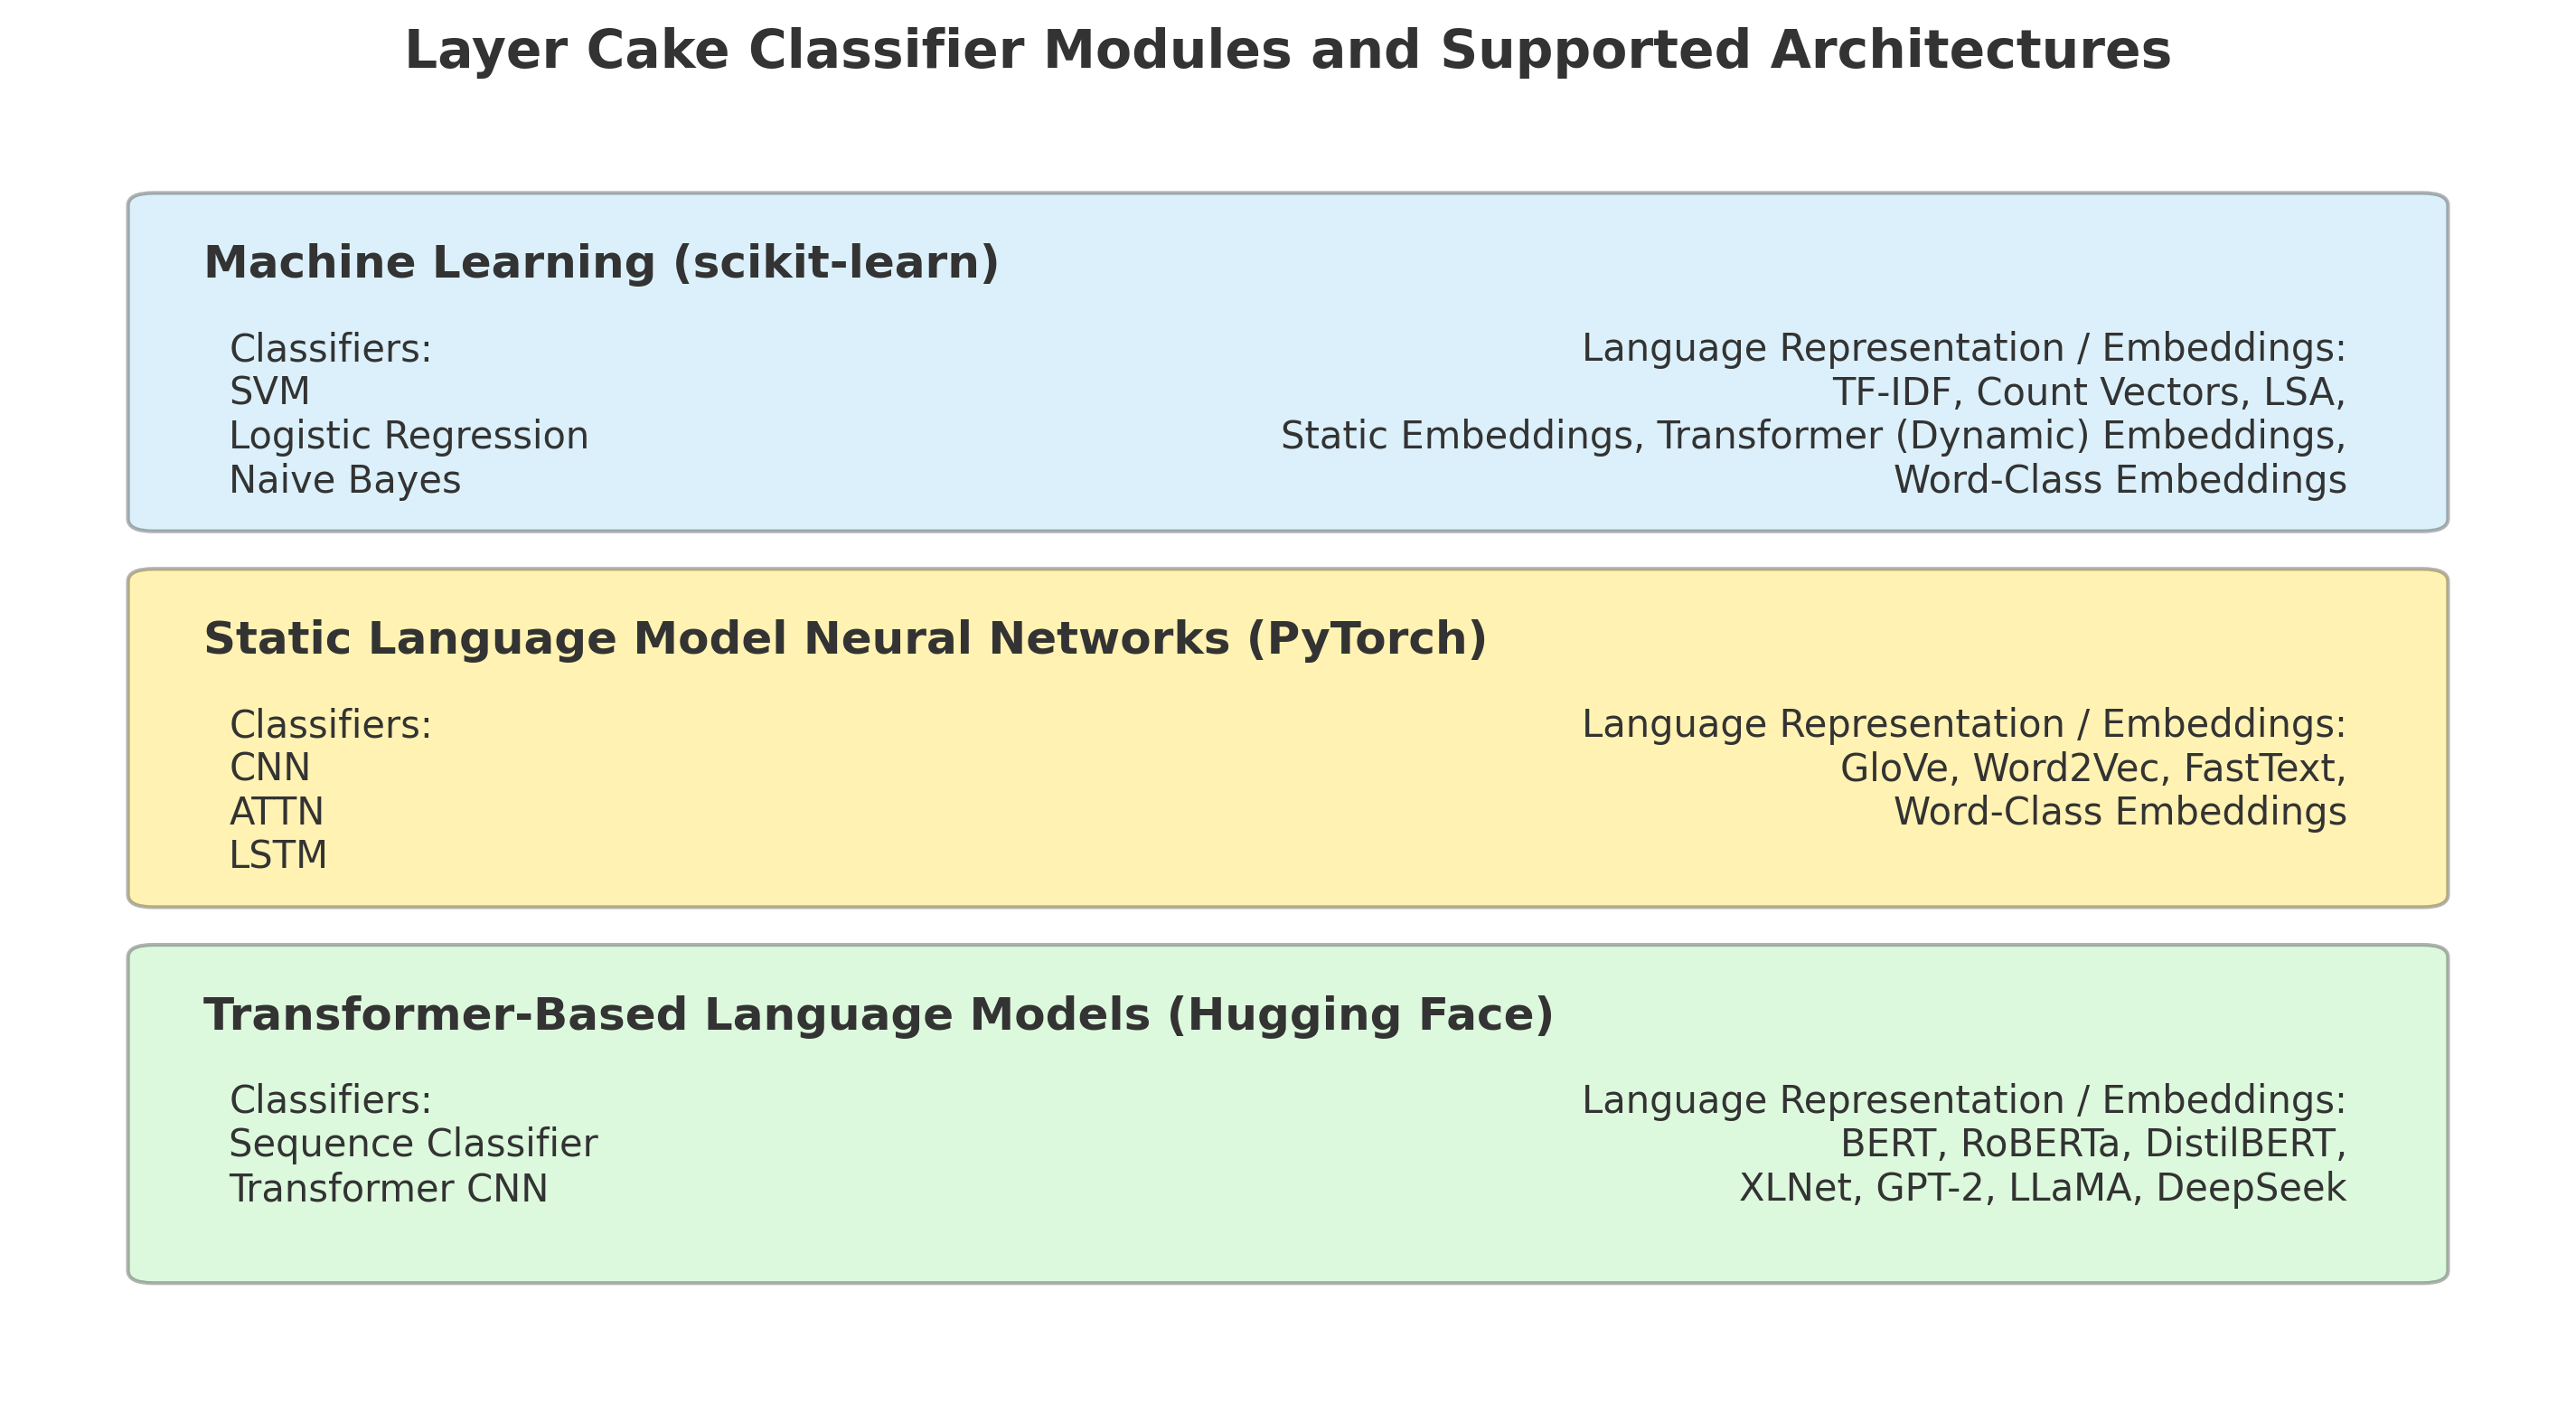
\includegraphics[width=0.9\textwidth]{pictures/fig1_layer_cake_classifier_modules.png} 
  \caption{\textit{Layer Cake Language Model Benchmarking System Modular Design}}
  \label{fig1}
\end{figure}




\subsection{Unique Contributions of this Research}

In brief, our work makes the following original contributions:

\begin{itemize}

\item We introduce a unified benchmarking framework for evaluating 12+ classifiers from both the ML and DL domains and using a variety of language representations from text vectorization, to word embeddings to transformers and LLMs, all tested against a variety of single-label and multi-label text classification datasets.
\item We systematically compare the tradeoffs between classifier performance and computational cost, showing that while LLM classifiers outperform traditional ML classifiers models by up to 12.73\% in Macro-F1 scores, they incur over 4000\% additional compute overhead (in training) compared to lightweight ML approaches.
\item We contribute detailed profiling of model training and inference time, highlighting how model architectural choices as well as different forms of language representation impact overall model performance and computational resource requirements.
\item We demonstrate empirically that incorporating Word-Class Embeddings (WCEs) with transformer-based classifiers not only fails to enhance their effectiveness but actively degrades their performance, resulting in lower Macro \& Micro F1 scores compared to using transformer embeddings alo
\item We provide practical guidance for researchers and practitioners by aligning model choice with available resources, expected latency, and classification complexity as well as explore the ability to augment existing models with embeddings from different vector spaces, showing that while these approaches can be effective in both an ML and static word embedding DL context, they are ineffective when combined with transformer models.
\end{itemize}


\subsection{Structure of this Work}
This work is structured as follows:
\begin{itemize}
	\setlength\itemsep{2pt} 
    \item \textit{Introduction}
    \item \textit{Research Context}: Historical perspectives on the evolution of various forms of language representation, brief introduction to transformer architecture and how they fit into this historical context, 
    \item \textit{Layer Cake Design and Experimental Setup}: explanation of the different Layer Cake modules and different classifiers they support, details on test data workflow and data preprocessing, different hyper-parameter settings, specifics on language representation forms as applicable, etc.  
    \item \textit{Results and Analysis}: detailed analysis of the data in terms of language representation forms, different types of classifiers. Global performance analysis, details on computational resource requirements
    \item \textit{Summary and Concluding Remarks}: summary analysis of data, recommended areas of further research
\end{itemize}


\section{Research Context: Language Representation, Transformers \& Text Classification}

We have witnessed many major milestones over the last few years in the advance of AI, fueled by the NLG tools that are built on top of foundational LLMs that continue to advance along many different dimensions, in particular with respect to support for multiple \textit{modalities} - i.e. pictures, text, sound, etc - as well as reasoning capabilities, sometimes referred to as \textit{chain-of-thought}.\footnote{Chain-Of-Thought, or COT, capabilities were first introduced in 2022 \cite{articlewei} but have more recently come to refer to the feature that many of the advanced language generation tools have integrated where the specific reasoning steps the model takes to arrive at a given response or conclusion are explicitly shown to the user as a sort of 'show your work' type of approach, opening up a whole new area of research and technological advancement with language generation tools specifically but certainly in AI more broadly as well.} The technological advancements necessary to facilitate this rapid advancement in language generation capabilities reflect decades of R\&D across the fields of linguistics, computer science, cognitive science, and certainly computing and infrastructure more broadly, the latter being a necessary condition for both the training, and utilization, of these advanced models. While there are many architectural innovations that have underpinned the evolution of language models over the last decade which are radically changing not just the AI landscape but the technology landscape writ large, one of the aspects of this architectural revolution that receives comparatively less attention is the means by which the underlying language that is processed by these models is \textit{represented} - the language that language models speak one could say. In the research literature this domain is called \textit{Language Representation (Learning)}, and this deficit in terms of the attention and focus it receives in the research community serves as a significant motivation for this work. 

Language representation in NLP however had much humbler beginnings, particularly at the early stages of NLP before neural networks when computational resources were at a premium. Early forms of language representation were based upon \textit{text vectorization} techniques such as one hot encoding, or Count Vectorization as it is sometimes called, a clasely related cousin to the very influential and still very popular form of text vectorization which takes into account the term's 'importance' within a given corpus called 'term-frequency inverse-document-frequency', or simply TF-IDF, which was introduced in 1972 \cite{sparckjones1972statistical}. But text vectorization approaches to language representation, which are still widely used today in particular within the context of classical machine learning (ML) NLP models, suffers from the so-called \textit{curse of dimensionality}, which is the computer science term given to the fact that as the number of dimensions increase in ML, the computation time tends to increase geometrically. This is a common problem with text vectorization approaches to language representation given that the feature space is defined by the size of the underlying dictionary which can be measure in the tens of thousands of words or terms, or with foreign languages from East Asia can be much larger in fact. Therefore vectorized text is usually submitted to a form of preprocessing to address this issue called \textit{feature reduction}, which looks to bring down the size of the input feature matrix to ML models while retaining as much of its predictive power as possible. Common feature reduction techniques such as Principle Component Analysis (PCA) \cite{pearson01111901} \cite{hotelling1933AnalysisOA}, as well as Latent Semantic Analysis, or LSA (or Latent Semantic Indexing, LSI) \cite{deerwester}, which leverages matrix \textit{eigendecomposition} in order to identify latent contextual (effectively semantic) relationships between words or terms in a document corpus, have been used for decades in classical NLP solves and are still widely used today.\footnote{We use LSA as one of our baseline feature reduction techniques in this work and our findings show that it remains an effective form of language representation, at least within the context of text classification.}


\subsection{Vector Space Models and Word Embeddings}

A different form of language representation emerged in the 1970s however, one that was informed by linguistics theory that looked to project language into a semantic space to facilitate document search and information retrieval - namely \textit{vector space models} \cite{salton1971smart} which form the basis of semantic spaces of meaning which provide the mathematical, geometrical, and linguistic foundations of \textit{word embeddings} which have emerged as the basic building blocks of LLMs. Word embeddings were first introduced in 2013 with Word2Vec \cite{mikolov} which uses DL along with word co-occurrence metrics to learn (word) embeddings by predicting words based on (local) word contexts\footnote{Window context being defined as for example 5 words before or after the current target word where 5 is configurable training parameter for the model.} using either a continuous bag of words (CBOW) approach where the model is optimized to predict the target word given a specific context, or a Skip-Gram predictive approach where the context of a word is predicted given the target word. GloVe (Global Vectors for Word Representation), another form of word embeddings introduced in 2014 \cite{pennington}, leverages both local and global word context to generate word embeddings, explicitly constructing a word co-occurrence matrix during training that records how often two words appear together within a context window across a corpus. It then factorizes this matrix via log-bilinear regression, optimizing a cost function which minimizes the difference between the dot product of two-word vectors and the logarithm of their co-occurrence count, effectively balancing both local and global co-occurrence statistics for the words in question. 

\begin{figure}[h!]
  \centering
  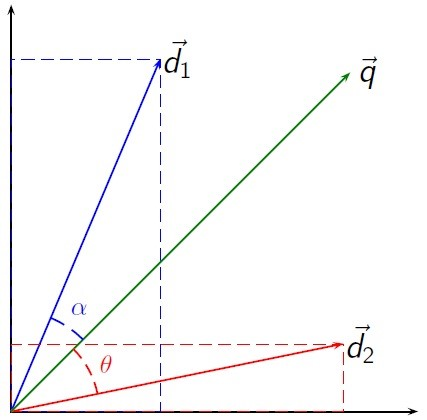
\includegraphics[width=0.3\textwidth]{pictures/fig2_doc_query_vector_space.jpg} 
  \caption{\textit{Document Similarity Query in Vector Space}}
  \label{fig2}
\end{figure}

FastText on the other hand, which first introduced in 2017 by Meta's AI team \cite{articleboja}, while very much related to Word2Vec in the sense that it is also a local co-occurrence computed (static) word embedding model, it is unique in that it introduces the concept of \textit{subwords}, or \textit{n-grams}, which allow the model to handle out of vocabulary terms (OOV) terms better by using subword embeddings to represent words that that were not identified in the pretraining corpus and therefore did not make it into the base model. With fastText embeddings, each word is represented not only by its word-level embedding but also by the embeddings of its subwords, enabling the language representation form to compute OOV words by composing them from the embeddings of their subwords. During training, FastText learns embeddings not just for entire words but also for their subword n-grams, and when creating the final vector for a word, FastText aggregates the word's subword embeddings (and its own embedding if available) into a single vector, resulting in embeddings that can handle morphologically rich languages better than Word2Vec which cannot break words into smaller units. 

Just like Word2Vec, FastText operates in a continuous Euclidean space (or more generally, a vector space) where words with similar meanings have vectors that are close together, as illustrated in in Figure~\ref{fig2}, and relationships between words can be modeled as linear transformations (e.g., "king $-$ man $+$ woman $\approx$ queen"). Since FastText breaks words into subword units (n-grams), this means that similar words (e.g., "running" and "runner") will have more similar vectors than they would in Word2Vec, due to shared subword components ("run"). FastText also constructs vectors geometrically, learning word and subword representations from their co-occurrence patterns in a latent space. This underlying geometrical configuration allows FastText to capture not just word-level relationships, but also similarities across words with shared subwords, such as morphological variations of the verb 'run', such that the words "run," "running," "runner" will have closer embeddings because of shared subwords. Because of its inherent subword design, FastText can produce embeddings for out-of-vocabulary (OOV) words from the embeddings of the subwords, in contrast to word-based language models, such as GloVe or Word2Vec, which typically represent OOV words with generic embedding placeholders like the mean embeddings across the whole dictionary of embeddings for example, facilitating the representation of words that were not included in any of the (pre) training corpora.

While text vectorization forms of language representation are explicit, algebraic constructions based on word frequencies in a given corpus, and each element in each document vector represents a distinct, interpretable feature, e.g. the presence or absence of a word in a feature space defined by the underlying dictionary of words for a given corpus, representing a direct frequency-based transformation of the raw data. Word embeddings on the other hand, live in a similarly defined feature space albeit it is not flat, it is hyper-dimensional with the number of dimensions defined again by the underlying dictionary of terms or words in a given model, within which the word (or subword) embeddings are calculated using various statistical measures along with DL models to compute vectors for each term in a continuous latent space. These vectors are learned through training on large corpora to capture semantic and syntactic relationships, resulting in dense, distributed representations where each dimension captures abstract relationships rather than direct counts. 

In essence, while TF-IDF and Count Vectorization build vectors through explicit algebraic transformations of text data, Word2Vec, FastText and GloVe embedding models use deep learning to geometrically place words into a latent vector space based on their usage (i.e. distribution) patterns in large corpora – with Word2Vec and FastText using local co-occurrence information to construct the vector space and GloVe using global context to construct the vector space. The text vectorization techniques yield clear, interpretable vectors (e.g., word counts), while the latter produces more abstract, dense representations. Ultimately, word embedding forms of language representation, which are critical foundational elements of all LLMs, rest on theoretical foundations which are borrowed from linguistics, namely the \textit{distributional hypothesis}, which states that words that appear in similar contexts have similar meanings, a principle which informs these word embedding models which are designed to place words that are found in similar contexts in the underlying corpora close to each other in the underlying latent (semantic) space within which the embeddings live. In other words, the model is trained to find the coordinates each word in a latent feature space where distances between vectors reflect their semantic similarity.

This connection between NLP and linguistics is long standing and rests at the very heart of language models in all their forms, resting on principles of semantics and morphology that were established primarily by Noam Chomsky in the middle of the last century. His most influential works with respect to computational linguistics perhaps being ''Three Models for the description of Language'', an article published in 1956 where he introduces formal grammars which now serve as the basis for computer language theory \cite{chomsky56}. In the book \textit{Syntactic Structures}, published in 1957, Chomsky introduces the notion of \textit{generative grammars} which serves as the basis for the hierarchy of languages which one of the most fundamental conceptual frameworks in Computation Theory \cite{Chomsky57}. Furthermore, in the and the book "Aspects of the Theory of Syntax" which was first published in 1965, Chomsky outlines the notion of generational grammars, distinguishing between deep and surface structures which in turn inform our modern notions of \textit{syntax} and \textit{semantics} which provide the theoretical foundations for linguistics which in turn drives much of the theoretical foundations of NLP \cite{chomsky65aspects}.

\begin{figure}[h!]
  \centering
  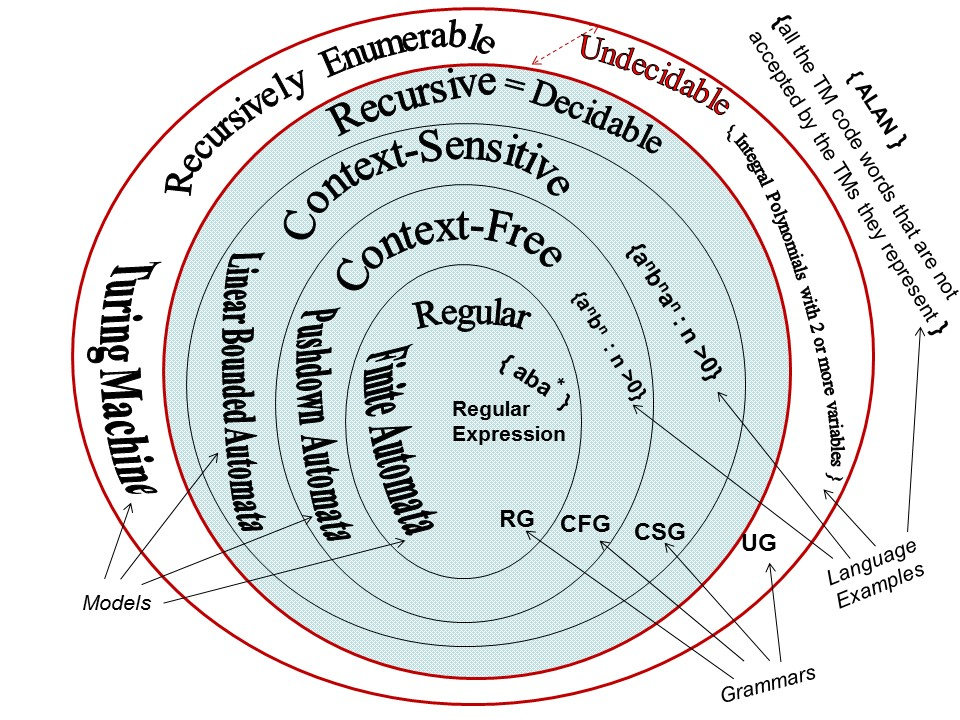
\includegraphics[width=0.6\textwidth]{pictures/fig3_chomsky_hierarchy_of_languages.png} 
  \caption{\textit{Chomsky Hierarchy of Languages \& Automata}}
  \label{fig3}
\end{figure}

One of the most prominent and prevalent principles that is borrowed from linguistics theory which is fundamental to language model training is the \textit{distributional hypothesis}, a core tenet of semantic theory whose origins go back to middle of the last century \cite{harris} \cite{firth} and which have been summarized beautifully by J.R. Firth, one of the scholars attributed to discovering this principle, as \textit{you shall know a word by the company it keeps}. This quite simple yet extraordinarily profound principle rests at the very heart of virtually all of the training methodologies for LLMs, and in some sense can be seen as a motivating factor for the introduction of the \textit{attention mechanism} \cite{bahdanau2016neuralmachinetranslationjointly} which is designed specifically to provide a more granular representation of a text sequence as a function of a) the semantic meaning of the pretrained token embeddings, and b) a representation of the underlying semantics of a given text sequence, sentence or passage. This additive semantic design strategy is arguably the very core of the technology innovation introduced by transformers in 2017 \cite{vaswani}.


\subsection{Attention Masking and Transformers}

It is fair to say that the introduction of word embeddings, an evolution and offshoot of vector space models, revolutionized language representation, allowing words to be represented as low-dimensional continuous vectors, but because they are static representations, i.e. are not context aware, they are relatively easy to work with from both a computational standpoint as well as from a language representation architecture standpoint. That is to say, given the clean mapping of a word to an embedding, one can enhance this structure relatively easily within the context of a neural network classifier by simply concatenating one embedding form with another, a technique that we test extensively within the context of our ML Classifier module where we test the efficacy of a variety of linear algebraic combinations of various forms of text vectorization, word and token embeddings, in conjunction with Word-Class embeddings \cite{moreo2021}, as well as feature reduction techniques such as LSA and document encoding using various embedding pooling strategies.

The static nature of these early language models, despite their ease of use in ML and DL contexts, nonetheless constrained their capabilities, i.e. they could not solve the \textit{polysemy} problem. Polysemy in linguistics is the term used to indicate that the meaning of a given word is very contextual, to the point where some words could have very different meanings if they are found in different contexts - like the word 'blue' for example which means the color blue in a sentence like 'the sky is blue' but means something else entirely if used in a sentence to describe someone's mood, like 'i was feeling very blue today'. This feature of language, really of all languages, is one of the most powerful means of the expression of ideas in fact, and the inability of these early models to be able to support this very important feature of language greatly constrains its power across a wide range of NLP problems. Conversely, the ability to support, to represent, this kind of nuance, opens the door to a vast array of capabilities across that very same spectrum of NLP problems, with these advanced language generation tools simply being the most widespread and most well known examples. This is arguably the most important innovation that comes with transformers and was precisely the motivation of the \textit{attention mechanism} \cite{bahdanau2016neuralmachinetranslationjointly} \cite{vaswani} which underpins transformer-based language models which facilitates the creation of a more complex semantic representation of language by breaking language down into tokens, or subwords, and then combining static representations of these tokens (embeddings) with positional information (also embeddings), in order to create what we call "context-aware" representations of language (again, embeddings). It is these advancements in language representation in fact that drive the power of the transformer architecture \cite{vaswani} which is the engine inside the hood of almost every modern LLMs in one form or another. 

While different types of transformers, and now different types of reasoning approaches and capabilities, have been the focus of much R\&D in the last few years, nonetheless all of these transformer architecture language models rely on a representation of language (text) that is first tokenized and then indexed, and then mapped to the underlying embedding structure, really placed in the underlying semantic space following the same linguistics theoretical principles described above, during model construction and pretraining. This embedding space is Euclidean, but is created in a unique way by each LLM based upon the given tokenization strategy, as well as the algorithm used by the LLM during training which optimizes the vector representations of tokens in the underlying semantic space. This is a major architectural difference from its predecessors, i.e. word embeddings, which are precomputed and static, at either the word or subword levels, and as such these models are less effective at handling the polysemy challenges which are fundamental to a proper understanding of language. But all of these different forms of embeddings which underpin language models in all of their forms are numeric representations of meaning in an underlying semantic space which facilitate a machine \textit{understanding} of the underlying language as it has been presented to the model which it in turn uses to generate outputs - whether these are natural language outputs for a chatbot based upon given input text (i.e. a \textit{prompt}), or a text summarization output based upon a given textual input, or in our case a classification label (or probability distribution of labels) based upon a given input doc or text sequence. These embeddings serve as search vectors in the underlying pretrained Euclidean space (\textit{semantic space} effectively, following \cite{worth}, which provide rich information to the underlying model. These pretrained embedding forms of language representation of course are very different from the earlier and more straightforward forms of language representation like \textit{text vectorization} which, while still remain a useful tool in some NLP solves, nonetheless remain divorced from semantics per se. 

Transformers begin processing text by tokenizing raw textual input into token IDs using a tokenizer. Transformer tokenizers are sophisticated and fundamental to language representation in LLMs so important to understand within the context of this research. The most prevalent types of tokenizers used with transformers are WordPiece, Byte-Pair Encoding, and SentencePiece tokenization, each of which is used by one or more language models that is tested with Layer Cake and each of which, like FastText's tokenization strategy, is a form of subword tokenization. WordPiece is a subword tokenization algorithm originally developed for Google's neural machine translation system \cite{schuster} \cite{wu}, and then used with BERT \cite{devlin-etal-2019-bert}. This tokenization strategy begins with a base vocabulary of individual characters and then iteratively builds a vocabulary of subwords by merging the most frequent pairs of characters and/or subwords. It is designed to keep common words intact, while splitting rare or unknown words into smaller, meaningful subword units. 

Byte Pair Encoding (BPE) on the other hand, introduced in 2016 \cite{sennrich-etal-2016-neural} and used in the GPT class of language models, is another subword tokenization method which was initially used for data compression and was then later adapted for NLP by the SentencePiece and GPT/GPT-2 models. Byte Pair Encoding begins with characters as tokens and then repeatedly merges the most frequent pair of tokens (characters or subwords) into a new tokens, continuing until reaching a desired vocabulary size. SentencePiece tokenization, used by T5 \cite{raffel2019exploring}, Albert \cite{lan2019albert} and XLNet \cite{yang2019xlnet} models, is a language-independent, unsupervised tokenization method introduced by Google in 2018 for neural text processing \cite{kudo2018sentencepiece}. Unlike traditional tokenizers, it does not rely on whitespace for tokenization, which is important when supporting languages that do not have clear word boundaries (e.g. a whitespace as is used in Western European languages to separate words for example) such as Japanese or Chinese. The output tokens include a special symbol (typically '\_') to denote spaces, allowing it to reconstruct the original text without external tokenizers.

Regardless of the tokenization strategy however, token IDs are generated for each specific language model based upon its underlying tokenization strategy and training corpus (and other algorithmic or parametric factors) and serve to map individual tokens to token embeddings, which are word embeddings for all intents and purposes just mapped to tokens rather than words. These token embeddings, like their word embedding counterparts in fact, are high-dimensional vector (e.g., 768-dim) that encodes the tokens semantic information within the semantic space that was constructed during the language model's development, or pretraining. The overall language model then, the fixed embedding layer that sits at the base of the transformer neural architecture, is a large embedding matrix of shape [vocab\_size, hidden\_size] that is again learned during pretraining and then typically fine-tuned during downstream tasks as we do in our research here with Layer Cake. However, this is not sufficient to achieve context-aware embeddings, which are the fundamental characteristic of transformers. 

In order to be truly context aware, the token embeddings must be coupled with additional information related to the specific position that the token is found, either within a sequence of tokens or within a given sentence, or document. The transformer uses this information as a \textit{mask} to generate embeddings which are a function of both the pretrained model \textit{and} the linguistic context within which the specific token, or sets of tokens, are found. This yields a model which allows for a better understanding of the \textit{meaning} of the specific token in that context as reflected in the dynamically generated embeddings that are created to represent that token by the transformer. This is where \textit{positional embeddings} come in, one of the most revolutionary parts of the original Transformer paper \cite{vaswani}. There are two main types of positional embeddings that are used by transformers (1) learned positional embeddings, where each position (e.g., 0-511) has a trainable vector stored in a matrix of shape [max\_position\_embeddings, hidden\_size], and (2) sinusoidal encodings, which use a deterministic function of sine and cosine waves to encode positions with different frequencies (the approach used in the original 2017 paper). In both cases, the output is a vector of the same shape as the token embedding, allowing element-wise addition.

These positional embeddings are then added to the token embeddings and then masked to yield the final set of embeddings which together \textit{represent} the text in question which are in turn fed into the transformer to generate 'context-aware' embeddings, facilitating the construction a semantic space which is much more nuanced, and much more granular, than the static word embedding language model predecessors that had no way to track or understand the context within which a given word, or token, is found in a given text or corpus. The final input embedding for each token is the sum of its token embedding and its corresponding positional embedding. This results in a matrix of shape [sequence\_length, hidden\_size], which is optionally passed through LayerNorm and Dropout before entering the first Transformer layer. This combined representation encodes both the semantic meaning of tokens and their relative positions, enabling the self-attention mechanism to reason about context and order, and ultimately solving the polysemy problem.

Furthermore, some language models also include what are known as segment embeddings, which provide information about which sentence, and which part of which sentence, each token belongs to necessary for training tasks like next-sentence prediction which require such information. Models such as BERT \cite{devlin-etal-2019-bert}, ALBERT \cite{lan2019albert}, XLNet \cite{yang2019xlnet}, and ELECTRA \cite{clark2020electra} all leverage some form of segment embeddings, learnable vectors that differentiate tokens belonging to different input sentences within a single input sequence. In these models, each token in the input sequence receives an additional segment embedding corresponding to the sentence or segment it belongs to, along with its token embedding (encoding its semantic meaning), and positional embedding (encoding its position). These three embeddings then - token, positional, and segment = are combined (element-wise summation) to form the final input embeddings that are provided to the transformer layers of the model, enabling the encoding of multi-sentence inputs which facilitates training on tasks like Next Sentence Prediction (NSP), question-answering, and sentence-pair classification.

\begin{figure}[h!]
	\centering
	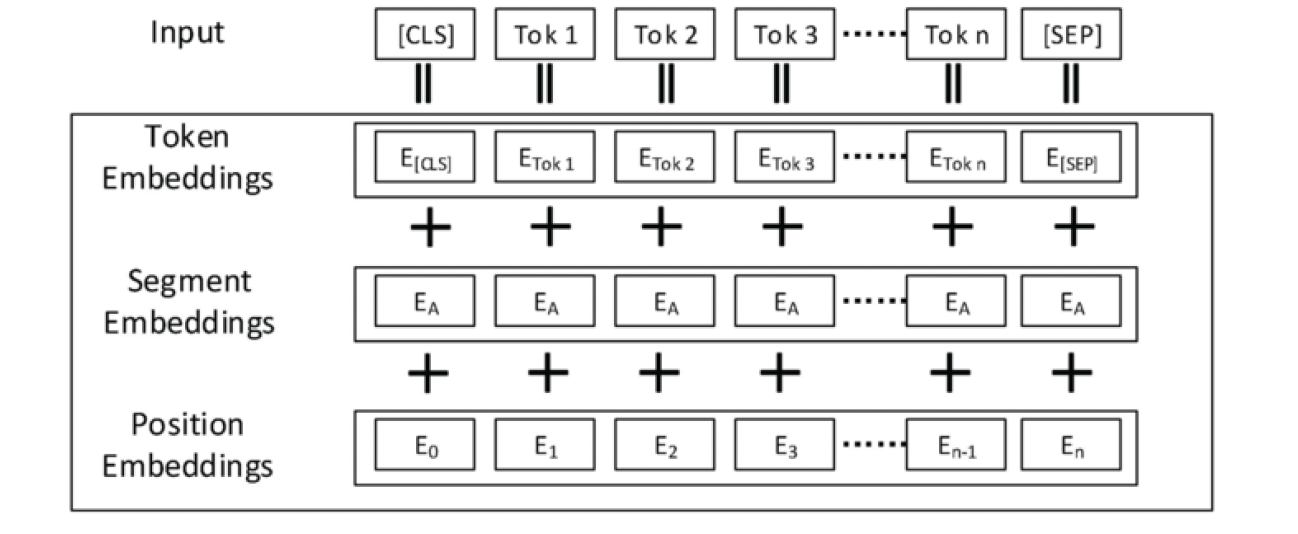
\includegraphics[width=0.9\textwidth]{pictures/fig4_llm_input_representation_embeddings.png}   
	\caption{\textit{LLM input representation - Token, Segment and Position embeddings \cite{zhang2022} }}
  	\label{fig4}
\end{figure}

It is the tokenization strategy, as well as the attention-based masking that transformers are typically known for, that combine together to produce the fine-grained powerful language models that have been the engine behind language generation tools and AI more broadly over the last 7 years. Some of the early influential deep learning approaches to NLP which leveraged transformer architectures and attention mechanisms to compute contextualized (dynamic) text representation forms of natural language were ELMo (Embeddings from Language Models), which was introduced in 2018 \cite{peters2018deep} which used bidirectional LSTM layers to generate contextualized embeddings, and then of course BERT (Bidirectional Encoder Representations from Transformers), which was introduced in 2019 \cite{devlin-etal-2019-bert} which uses a unique, bidirectional approach to generating contextualized embeddings which, in both its original form and in many branches of derivation, is still a common tool used for a variety of NLP solves such as sentiment analysis, question answering, and named entity recognition. 

Almost all the most popular and influential LLMs in use right now leverage this transformer, attention-based architecture which has replaced virtually all of the prior DL, neural network based architectures that came before it (e.g. RNNs with self-attention mechanisms or Convolutional Neural Networks or CNNs), underpinning many state-of-the-art results in machine translation, text classification \cite{devlin-etal-2019-bert}, natural language understanding, and (natural) language generation tools \cite{radford2019language} and applications. These models, and their associated platforms and operational infrastructures, have pushed the boundaries of language generation and NLP more broadly, greatly enhancing AI capabilities and enabling the development of powerful NLP applications such as conversational agents, document summarization, and ultimately LLMs which show surprising versatility.

\subsection{Text Classification, Deep Learning \& Word-Class Embeddings}

Text classification, the core NLP problem that is analyzed and tested with this work as a means to test the different computational resource requirements of the various language models and associated language representation forms, is one of the foundational problems in (NLP) that has applications across the technology and software landscape - ranging from topic classification for news and other related research sites, to spam detection and email filtering, to content moderation and sentiment analysis, to fraud and malware detection in the cyber security space. The problem, as we frame it here, involves assigning predefined labels to textual data and then building and training models to predict how new text (documents) are to be classified based upon historical data that has been fed into the model, i.e. a form of supervised training which is a very common, and very effective, means of model training and construction. While there have been a variety of good research surveys written that look at the problem of text classification within the context of different DL architectures and/or LLMs - for example relatively early studies looking at pre-trained language models for NLP more broadly in 2020, \cite{qiu2020pre}, another focused on deep learning approaches for text classification specifically \cite{minaee2021deep}, and another very thorough study that looks at the effectiveness of various optimization techniques and hyperparameter tuning applied to the text classification problem focused exclusively on LLMs published in late 2024 \cite{trust2024study}. However, these studies do not include classical ML approaches to text classification in their work, and while there do exist some notable text classification research surveys that do include both ML and DL approaches, e.g. \cite{liu2019roberta}, these studies are dated and do not account for the increased size and compute requirements for the more modern LLMs, properties that are becoming of increasing importance given the need for, and expense and scarcity of, GPU clusters at the size and scale necessary to build, train tune such large and computationally resource dependent language models. With this work, and with the Layer Cake benchmarking platform that comes with it, we address this gap in research by directly comparing CPU bound, classical ML classifiers alongside GPU bound DL text classifiers which include both transformer-based language model classifiers and static word (and subword) based language models - such as Word2Vec, FastText and GloVe - shedding much needed light on the relative computational resource requirements for each of these types of classifiers, for each of these different forms of language representation (language models effectively).  

Research related to Text Classification, one of the major themes of this work, follows a similar trajectory as language representation described above, with early solutions leveraging various forms of text vectorization like TF-IDF \cite{sparckjones1972statistical} and feature reduction techniques such as LSA/LSI \cite{deerwester} used in tandem with classical Machine Learning models such as Support Vector Machines \cite{joachims1998text}, or simpler methods such as Logistic Regression or Naive Bayes \cite{mccallum1998comparison}. A good summary of the various ML approaches to text classification can be found in the 2002 work by Fabrizio Sebastiani \cite{sebastiani2002machine}, a paper which surveys different Machine Learning approaches to the problem of text classification before the proliferation of neural networks and deep learning techniques in NLP, also focusing on document (language) representation, classifier construction and evaluation as we do here. With the advent of deep learning and neural networks came the introduction of (static) word embedding language models which were trained in this setting as well as the introduction of various neural network architectures that were proven to be effective with text classification problems specifically - in particular work related to Convolutional Neural Networks (CNN) \cite{yoon2014convolutional} \cite{zhang2015character}, Long Short-Term Memory networks (LSTM) \cite{zang2021research}, and Attention based neural networks (ATTN) \cite{liuguo2019bidirectional}, each of which is used as benchmark classifiers with Layer Cake to test different static word embedding language models (Word2Vec, GloVe and Fasttext) in a deep learning setting following \cite{moreo2021}. Each of these neural models is tested with each of the static embedding language models using a variety of hyperparameter settings and generally speaking these models hold up well relative to the transformer and ML classifiers that they are compared against, while requiring considerably less computational resources than the transformer-based classifiers we test.

What closely followed this research, related to text classification in particular and which provided some of the (initial) motivation for this work, were the introduction of Word-Class Embeddings (WCE), which were shown to be effective - for text classification problems - when combined with static language model embeddings. WCEs are effectively a pre-computed class vector, sized based on the number of classes or labels in the text classification problem, that maps each specific term or word of the language model dictionary to each of the predefined class labels, calculated using a variety of techniques that range from the straight probabilistic to the use of informational theoretical primitives such as pointwise mutual information \cite{moreo2021}. Confining the WCEs to their own vector space allows for them to be added to pretrained (static) word embeddings quite elegantly, and their work shows that WCEs, when combined with static language model generated embeddings, do in fact significantly improve the performance of classifiers across the ML and DL spectrum - SVMs, CNNs, LSTMs and ATTN based classifiers specifically. We found in our testing however, that WCEs (really Token Class Embeddings, or TCEs, within the context of Transformers), which again are computed in their own vector space which is independent from the vector (semantic) space that LLMs use to compute its embeddings, did not contribute to the performance of the classifiers at all. In fact, what we found was that no matter what type of linear algebraic operation we used to combine the TCEs with the transformer generated embeddings (dot product, addition, concatenation), in all cases the classifier resulting Macro-F1 and Micro-F1 scores actually \textit{decreased}. We suspect that this is due to the fact that the transformer models are so complex and tightly coupled with their precomputed embeddings structure, i.e. tightly coupled to the underlying semantic space of the underlying language models, that the addition (or concatenation or multiplication) of embeddings which are computed in an independent vector space only served as to confuse the model during training, hence the decrease in performance of the classifiers when the TCEs were added. 

The next stage of evolution for deep learning, embedding based classifiers is of course the transformer based models, which use multiple attention heads along with a more sophisticated representation of the underlying text which captures the specific context within which the token is found in order to generate context-aware, dynamic word embeddings that solve the polysemy as well as the out-of-vocabulary (OOV) problem in NLP and generally provide much greater granularity and specificity when navigating through the underlying semantic space which is bound by the dictionary of tokens for the given language model and is defined by the training algorithm and pre-trained data which the language model was trained on.  Some of the earliest transformer models that were shown to be effective for text classification problems were BERT, which stands for Bidirectional Encoder Representations from Transformers which was released in 2019 \cite{devlin-etal-2019-bert}, as well as derivations thereof: like RoBERTa, or Robustly Optimized BERT Pretraining Approach which was released shortly after BERT also in 2019 \cite{liu2019roberta}, as well as DistilBERT, a \textit{distilled} \cite{hinton2015distilling} variant of BERT which while smaller and more efficient computationally, was shown to be (and confirmed in this study) just as effective \cite{sanh2020distilbert}for text classification. 

\begin{figure}[h!]
	\centering
	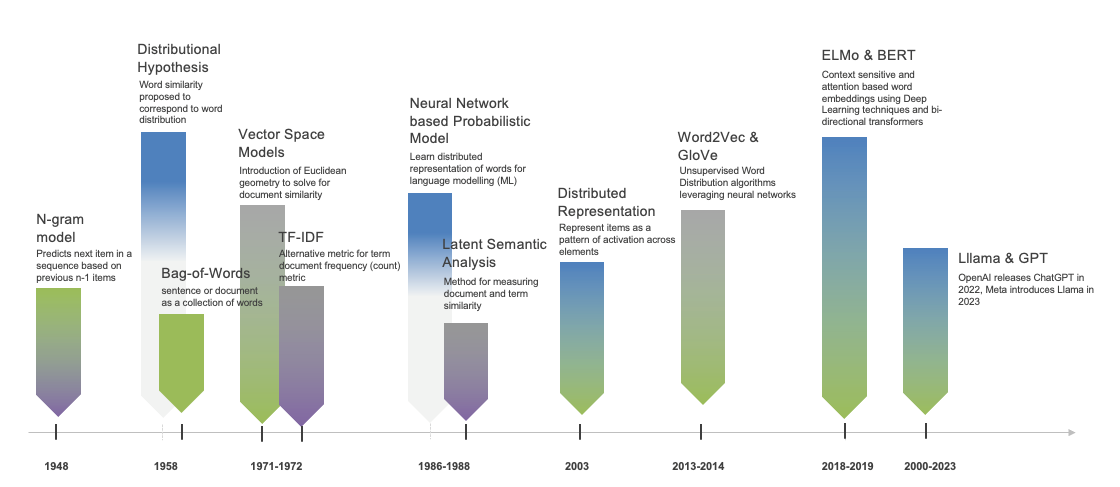
\includegraphics[width=1\textwidth,height=6cm]{pictures/fig5_nlp_timeline.png} 
	\caption{\textit{NLP Major Milestones Timeline}}
	\label{fig5}
\end{figure}

These transformer models, each with its own nuanced training approach and transformer architecture, along with the GPT-3 model \cite{articlebrown}, as well as an XLNet model \cite{yang2019xlnet}, along with smaller language models from both the Llama \cite{touvron2023llama} and DeepSeek family \cite{articlebi}, were included in the benchmarking that was performed in this research, each of which was tested across a variety of classifiers and each of which was shown to be effective for text classification, although the computational requirements of the transformer models significantly surpassed their static neural network counterparts, metrics and insights that are unique to this study.


\section{Layer Cake Design \& Experimental Setup}

Layer Cake can be viewed as an expanded NLP pipeline that includes support for multiple datasets, multiple forms of language representation, along with support for multiple classifiers from both classical Machine Learning as well as more advanced Deep Learning architectures. The nature of the different classifiers, given how they optimize and solve for the text classification problem in question, determines the forms of language representation that can be used for that given classifier as well as the data preprocessing steps necessary to configure such language representation forms. The overall dataflow and modular architecture of Layer Cake is depicted in Figure \ref{fig6}. While our test methodology generally follows \cite{moreo2021}, we extend the footprint significantly in terms of the ML classifiers and language models we test, the forms of language representation that we use for the ML testing, and the extension of the testing framework into transformers. All of the code is available on GitHub for further research or the reproduction of results, with both MacOS (MPS) and Ubuntu Linux (CUDA) systems supported.\footnote{https://github.com/pworth1971/layer-cake}

Given the scope of Layer Cake, and the NLP pipeline dependencies that are characteristic of the different types of classifiers it supports as mentioned above, Layer Cake is split into three different modules for testing:
\begin{enumerate}
    \item \textit{ML Classifier Testing}: A script for ML testing which supports Support Vector Machines, Logistic Regression and Naive Bayes classifiers,\footnote{The Naive Bayes classifiers have some restrictions given the dependency on positive numbers, some of the language model embeddings do not satisfy this requirement and so are not run through this classifier.}
    \item \textit{Static LM DL Testing}: A script for DL classifier testing that is designed for static word embedding language models which include Word2Vec, FastText and GloVe embeddings, testing each of the language models with different hyperparameters within hand crafted PyTorch CNN, ATTN and LSTM neural architectures, and
    \item \textit{Transformer LM DL Testing}: a second DL test script which supports transformer models (aka dynamic or context-aware embeddings) which leverages the Hugging Face libraries using language models from the BERT, RoBERTa, DistilBERT, GPT-3, XLNet, Llama and DeepSeek language families in conjunction with a custom CNN classifier (designed after the CNN architecture used for the static word embedding language models), as well as Hugging Face SequenceClassifiers which are uniquely designed for each specific language model and can be used via a standard Hugging Face API.
\end{enumerate}

\begin{figure}[h!]
	\centering
	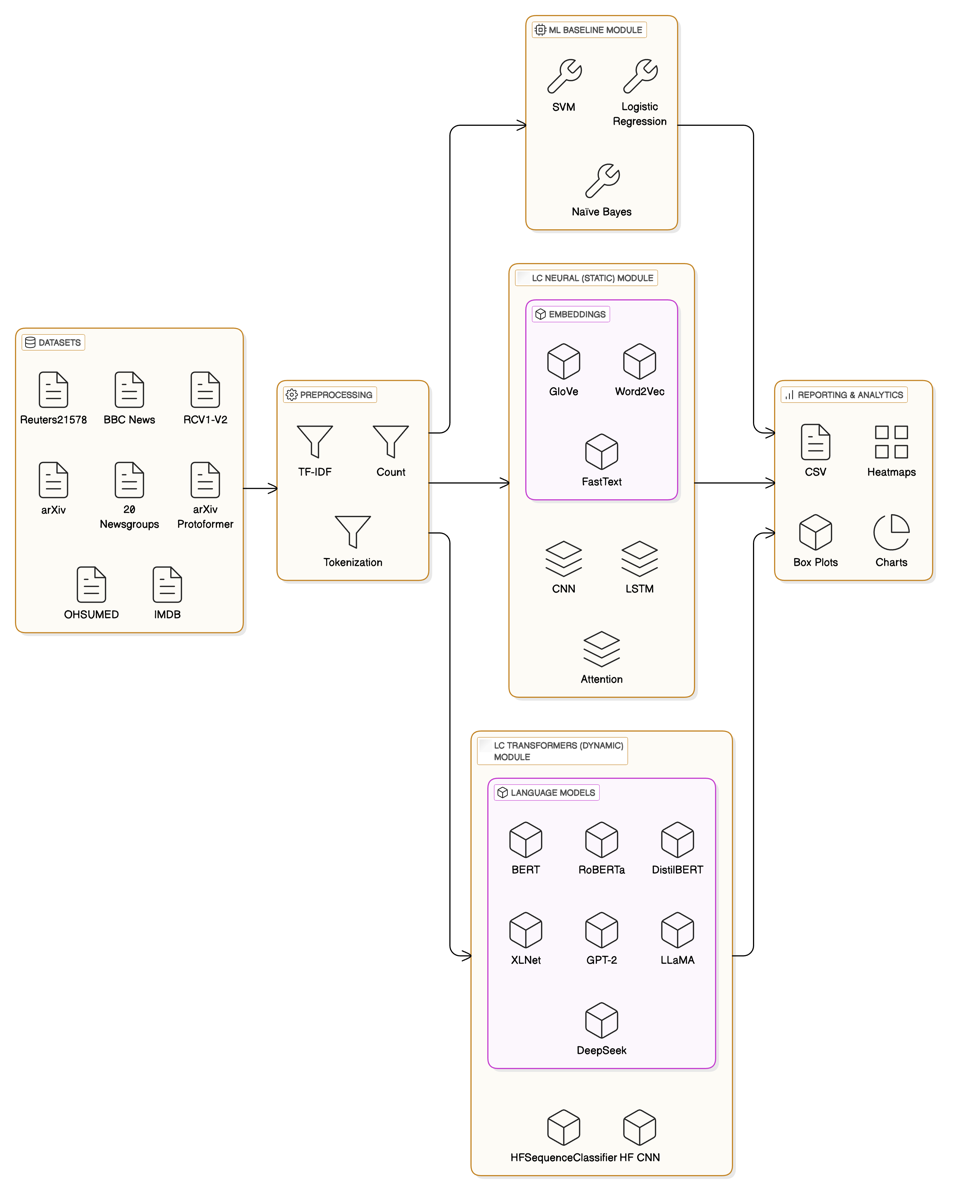
\includegraphics[width=0.95\textwidth]{pictures/fig6_lc_design.png} 
	\caption{\textit{Layer Cake Testing Architecture \& Data Pipelines}}
	\label{fig6}
\end{figure}

Each of the test modules are run with various hyperparameter settings and configurations, and each of these modules include support for multiple classifiers, furthermore each classifier is tested with different language models and datasets and hyperparameters, and in addition the ML classifiers are all tested with a a variety of language representation forms along with the different language models. All metrics and analytics for every test run are written to a log database (a tab delimited text file), which supports a variety of metrics (see below) and is used for generating the summary data, analysis, charts and plots that are included in this work. The log data includes information about classifier construction or build times, the various hyperparameter settings that are used, the underlying CPU and GPU architecture, the underlying OS and memory characteristics, as well as the version of the code that is executed. 

The ML baseline testing module (ml\_classification\_test\_version.py) module covers the baseline machine learning classifiers that we test with, namely Support Vector Machines and Logistic Regression and Naive Bayes classifiers. We use the scikit-learn libraries\footnote{https://scikit-learn.org/stable/} to build and run the respective classifiers, namely the LinearSVC, LogisticRegression, and MultinomialNB, using a OneVsRestClassifier approach for the multi-label datasets. This code is CPU bound for the most part, although the transformer embedding computations of the different dataset and language model combinations are GPU bound. This code ran on an Ubuntu Linux system with a single GPU system with the same system specification as described above. The final set of test runs for the ML classifiers were run on a 2023 MacBook Pro with an Apple M3 chip and 128 GB of RAM.\footnote{The Deep Seek model we tested does not support MacOS so that language model is not included in our ML testing.} These MacOS machines have their own GPU, which Apple calls a Metal Performance Shader (MPS), which is optimized for both graphics and compute (i.e. Deep Learning) capabilities. PyTorch has support for this environment (MPS), and we leverage this extensively for the language representation construction code for the different language models that we feed into the ML classifiers. The ML test code, as well as the DL test scripts in fact, are designed and tested to work on both the MacOS as well as Ubuntu Linux (22.04 x86) environment.\footnote{While not as performant as the CUDA libraries on the Ubuntu Linux environment, it’s not clear whether or not this is a hardware, or a software constraint given that CUDA support and capabilities remain the industry standard and clearly outperform MPS capabilities both in terms of function as well as performance.}

The neural model classifiers that are designed for the static word embedding language models - Word2Vec, fastText and GloVe - are GPU bound (CUDA), although they also run on MPS / Apple Silicon. The neural classifiers used for this testing are hand crafted using a very thin PyTorch layered design which is inherited from \cite{moreo2021} that supports custom designed CNN, ATTN and LSTM based neural classifiers. Figure 7 below is a sample CNN PyTorch classifier we use in this work. These classifiers do not support any form of parallelism however, and therefore the Embeddings must be small enough to fit on a single GPU. The transformer language models on the other hand are integrated and tested with a separate script that leverages the Hugging Face APIs and supports a CNN classifier that is modeled after the CNN architecture we use to test the static word embedding language models (see Figure 8 for an example), as well as a Hugging Face built in Sequence Classifier that supports the various transformer language models that are in scope for Layer Cake.  The transformer classifier test script does support a simple form of PyTorch parallelism known as DataParallel\footnote{For a more detailed treatment of parallelism using PyTorch and/or Hugging Face we suggest https://huggingface.co/docs/transformers/v4.13.0/en/parallelism.}, where the model is replicated on all of the in-scope GPUs, data is doled out equally across the GPUs during training, in parallel, and then model updates are synchronized after each training step, which is not as sophisticated as the Distributed Data Parallel approach but is simpler to implement and still takes advantage of multiple GPUs if available \cite{li2020pytorchdistributedexperiencesaccelerating}. 

Both of the Deep Learning test modules were run on a Linux Ubuntu system using CUDA libraries, with the exception of the RCV1 dataset which, given its size, was tested on the MacOS test system outlined above. The Ubuntu variant that we ran on had the following system specifications:

\begin{itemize}
	\setlength\itemsep{1pt}

    \item 	OS: Ubuntu Linux version 22.04, x86 architecture
	\item 	CPUs: 64 physical, 128 logical; 512 GB RAM (memory)
	\item 	GPUs: 4 NVIDIA RTX 6000 Ada Generation, 48GB of Memory each
	\item 	CUDA 12.4
	\item 	Python 3.10 (DeepSeek model dependencies)

	\begin{itemize}
    	\item PyTorch 1.4.1 
		\item Transformers 1.45.2 
		\item 	Sklearn 1.6.1
		\end{itemize}
\end{itemize}

One of the important insights that this research sheds light on is the impact of, and relationship between, the requisite form of language representation for each of the classifiers we test with. For example, when working with the transformer classifiers, the first set of layers in the model (Embedding layers) are automatically set by the underlying transformer model itself and cannot be modified or extended in any way without breaking the model, whereas the DL classifiers we use for the static language models (which come in CNN, ATTN and LSTM variants) have more flexibility with how this Embedding layer is set up given that the embeddings are static and are not modified during model training. Furthermore, the ML classifiers, given their more straightforward mathematical design, have significantly more flexibility with respect to how the underlying data can be represented, hence the ability to test various forms of language representation in this context. 

We see these model constraints born out for example in our attempts at integrate WCEs (really TCEs, or Token Class Embeddings within the context of transformers) into the Hugging Face classifiers designed to support transformer-based language models. This was in fact the original motivation for this work was to test the efficacy of integrating varying types of embeddings that were generated outside of the model within the context of text classification problem, work which is the very crux of the \cite{moreo2021} study. Given the constraints of the underlying Hugging Face transformer models however, as well as the tight coupling between the initial embedding layer and the run-time token embedding computation i.e. the context-sensitive, attention mechanism which is arguably the fundamental characteristic of transformers, the integration of TCEs into the model actually detracted from the model performance, a result that was both unexpected and also telling in terms of the integration capabilities of transformers as they are currently architected as a self-contained system. Furthermore, these classifier architectural differences not only drive different approaches to language representation, but also have significant performance implications, a fact that is well known but not so well quantified in terms of cost-benefit, one of the unique contributions of this work. Quantifying the computational cost for training these models, both in terms of types and quantities of GPUs required to train the underlying model (none in the case of ML classifiers), as well as overall classifier model training times \footnote{This is what we measure as the \textit{timelapse} value in the tables and results throughout. This is the amount of time, in milliseconds, that it takes to train the mode, excluding all the data preparation and preprocessing times.}, is one of the core attributes of Layer Cake which distinguishes this work.

What is important to understand with respect to the underlying computational requirements of the different Layer Cake test modules, especially within the context of the model construction time analysis below, is that:
\begin{enumerate}
	\setlength\itemsep{2pt} % <-- tightens spacing between items
    \item the ML testing is CPU bound,
    \item the neural model testing is all GPU bound, single GPU, and 
    \item the transformer model testing supports GPU parallelism (4 GPUs)
\end{enumerate}

While the DL classifiers for the static word embedding language models do not support and form of GPU parallelism, i.e. they run on a single GPU, the transformer based pretrained language model testing on the other hand does use the most basic form of PyTorch parallelism called  DataParallel.\footnote{See https://pytorch.org/docs/stable/generated/torch.nn.DataParallel.html.} This means that the static DL classifiers we test with that are designed for precomputed and fixed word embeddings (in CNN, LSTM and ATTN variants), use 1/4 the amount of GPU resources than the transformer-based classifiers we test with. While studies show that the more advanced form of PyTorch parallelism, Distributed Data Parallel, scales linearly with the number of GPUs \cite{li2020pytorchdistributedexperiencesaccelerating}, we most certainly found a significant uptick in GPU resource requirements when using the transformer-based approach, results that are embedded in the timelapse analysis we cover below.

Furthermore, another important distinction between the transformer-based DL classifiers and their more simple PyTorch cousins that are designed for static word embedding language models, is that they, at least as Hugging Face has designed them, do not support either optimizations or customizations of the initial Embedding Layers of the transformer parts of the neural architectures (if we wanted to limit the size of the token embeddings used for example), nor did they support the integration of TCEs (token class embeddings, the tokenized version of WCEs), either at the Embedding Layer through concatenation as we do with the static DL word embedding classifiers, or even in the forward pass as the dynamic embeddings are computed and then fed into the classifier head (see Figures 7 and 8 for a readout of the neural architectures of the respective CNN classifiers). Regardless of the linear algebraic form of integration that we tried, regardless of where in the neural model we tried it, these TCEs that are constructed in their own latent vector space and have shown to be effective in text classification problems in both classical ML classifiers andDL classifiers that are designed to support static language model embeddings, as we report here which is consistent with \cite{moreo2021}, not only did their integration \textit{not} improve the classifier model performance (in terms of Macro-F1 and Micro-F1 scores), but it actually \textit{detracted} from the model performance. We suspect this is due to the very nuanced and granular method by which these transformer models generate embeddings, a method which is clearly very sensitive to outside interference which is in effect what the TCEs are in this context. The models are powerful but they are also hard to integrate with and customize, again at least in the Hugging Face model variants we used in this research.


\subsection{Supported Metrics}
Primarily we look at macro-f1 and micro-f1 scores for the different classifier, language model, and representation form test runs, but we also track precision, recall, accuracy, Hamming Loss and Jaccard Index numbers for each model run as well, although these latter metrics are not used in our analysis. Note that we use the macro-f1 score to determine whether or not our neural models are improving and to determine whether or not we have met our early-stop condition. We briefly cover how these metrics are calculated below. As a refresher, we outline how we compute these metrics within the context of Layer Cake benchmarking. 

\subsubsection{Precision}
Precision measures the accuracy of positive predictions. It is the ratio of correctly predicted positive observations to the total predicted positives, or 

\begin{align*}
    Precision=\frac{TP}{TP+FP}
\end{align*}
where TP is true positives and FP is false positives. 

\subsubsection{Recall}
Recall (sensitivity) on the other hand, measures the ability of a model to find all the relevant cases (i.e., True Positives) within a dataset. It is the ratio of correctly predicted positive observations to all observations in the actual class, or mathematically:
\begin{align*}
    Recall=\frac{TP}{TP+FN}
\end{align*}

\subsubsection{Macro and Micro F1 Score}
The F1 score is a more widely used measure of predictive performance given that incorporates precision and recall into one measure using the harmonic mean, defined mathematically as: 
\begin{align*}
  F1=2\times \frac{Precision\times Recall}{Precision+Recall}  
\end{align*}
The macro variant of the F1 score, i.e. macro-f1, uses the arithmetic mean of all the per-class F1 scores, treating all classes equally regardless of their support - i.,e. the number of times the class is found in the training data set. This unweighted average F1 Score across classes is defined mathematically as:
\begin{align*}
    Macro\text{-}F1=\frac{1}{N }\sum_{i=1}^{N} 2\times \frac{Precision_i\times Recall_i}{Precision_i+Recall_i} 
\end{align*}
Where Precision and Recall are calculated as outlined above and N is the number of classes.

The micro-F1 Score on the other hand uses the class specific contribution to compute the average F1 score, measuring the aggregate contributions of all classes with respect to the average score, or mathematically:

\begin{align*}
    Micro\text{-}F1=2\times \frac{Micro \text{-}Precision\times Micro\text{-}Recall}{Micro\text{-}Precision+Micro\text{-}Recall}
\end{align*}
Where Micro-Precision and Micro-Recall are the precision and recall calculated globally.


\subsection{Language Representation and Test Workflow}
The baseline ML classifiers we use within the context of this work are Support Vector Machines, Logistic Regression and Naive Bayes models, the first two of which effectively work by optimally separated the underlying dataset representation, in high dimensional space defined by the space of words in the underlying dataset. The Naïve Bayes model is a pure probabilistic approach and while its use is limited, due to the constraint that it must work in the positive real number space, it nonetheless provides a nice probabilistic baseline for our analysis. 

The neural models come in two forms - the neural models that are designed to work with static word embedding language models such as GloVe and Word2Vec (and FastText), and then the transformer architecture models which are much more sophisticated and computationally intensive than their static model counterparts. For these latter models we leverage the Hugging Face APIs which not only provide the ability to work with the various models that are included in this study but also come with predesigned Sequence Classifier models that are designed specifically for sequence, i.e. text or natural language, classification.

The train, validation and test split numbers for each of the datasets is listed in the table below, and is broken down by classifier as each classifier has slightly different preprocessing logic, with the neural networks requiring a validation data set set aside from the training data to test the training epochs. Note that we, following \cite{moreo2021}, use the standard 'Lewis Split' for the RCV-1 dataset \cite{lewis2004}, allowing us to evaluate our results more precisely against prior research.

\begin{table}[h!]
\centering
\scriptsize
\caption{Dataset Summary by Classifier Type}
\renewcommand{\arraystretch}{1.1}
\begin{tabularx}{\textwidth}{@{}p{1.6cm}p{2.1cm}lllrrr>{\raggedleft\arraybackslash}X@{}}
\toprule
\textbf{Classifier Type} & \textbf{Dataset} & \textbf{Type} & \textbf{Classes} & \textbf{Docs} & \textbf{Train} & \textbf{Val} & \textbf{Test} & \textbf{Train-Test Split} \\
\midrule
ML & bbc-news & single-label & 5 & 1,490 & 1,229 & NA & 261 & 82.48\% \\
   & arxiv\_protoformer & single-label & 10 & 100,000 & 82,500 & NA & 17,500 & 82.50\% \\
   & rcv1 & multi-label & 101 & 804,414 & 23,149 & NA & 781,265 & 2.88\% \\
   & reuters21578 & multi-label & 115 & 12,902 & 9,603 & NA & 3,299 & 74.43\% \\
   & 20newsgroups & single-label & 20 & 18,846 & 11,314 & NA & 7,532 & 60.03\% \\
   & arxiv & multi-label & 58 & 14,500 & 11,962 & NA & 2,538 & 82.50\% \\
   & imdb & single-label & 2 & 50,000 & 25,000 & NA & 25,000 & 50.00\% \\
   & ohsumed & multi-label & 23 & 34,389 & 24,061 & NA & 10,328 & 69.97\% \\
\midrule
DL (static-word) & bbc-news & single-label & 5 & 1,490 & 984 & 245 & 261 & 82.48\% \\
   & arxiv\_protoformer & single-label & 10 & 100,000 & 66,000 & 16,500 & 17,500 & 82.50\% \\
   & rcv1 & multi-label & 101 & 804,414 & 18,520 & 4,629 & 781,265 & 2.88\% \\
   & reuters21578 & multi-label & 115 & 12,902 & 7,683 & 1,920 & 3,299 & 74.43\% \\
   & 20newsgroups & single-label & 20 & 18,846 & 9,052 & 2,262 & 7,532 & 60.03\% \\
   & arxiv & multi-label & 58 & 14,500 & 9,570 & 2,392 & 2,538 & 82.50\% \\
   & imdb & single-label & 2 & 50,000 & 20,000 & 5,000 & 25,000 & 50.00\% \\
   & ohsumed & multi-label & 23 & 34,389 & 19,249 & 4,812 & 10,328 & 69.97\% \\
\midrule
DL (dynamic-transformers) & bbc-news & single-label & 5 & 1,490 & 1,014 & 215 & 261 & 82.48\% \\
   & arxiv\_protoformer & single-label & 10 & 100,000 & 68,063 & 14,437 & 17,500 & 82.50\% \\
   & rcv1 & multi-label & 101 & 804,414 & 19,098 & 4,051 & 781,265 & 2.88\% \\
   & reuters21578 & multi-label & 115 & 12,902 & 7,923 & 1,680 & 3,299 & 74.43\% \\
   & 20newsgroups & single-label & 20 & 18,846 & 9,335 & 1,979 & 7,532 & 60.03\% \\
   & arxiv & multi-label & 58 & 14,500 & 9,869 & 2,093 & 2,538 & 82.50\% \\
   & imdb & single-label & 2 & 50,000 & 20,625 & 4,375 & 25,000 & 50.00\% \\
   & ohsumed & multi-label & 23 & 34,389 & 19,851 & 4,210 & 10,328 & 69.97\% \\
\bottomrule
\end{tabularx}
\end{table}


\subsubsection{Machine Learning Approaches (Baseline Testing)}

With our baseline testing, we experiment on a variety of forms of language representation given that the model design is straightforward enough, and flexible enough, to support a variety of different language representation methods. These models are constructed using the base python sklearn libraries and as such they are CPU bound, as opposed to the GPU bound neural models that we describe below. While we primarily look at these baseline ML classifiers as baseline test cases to be viewed against the backdrop of their more sophisticated – and computationally intensive – counterparts, these models are nonetheless effective in and of themselves as standalone text classification solutions and are very easy to work with and perform very well on small and medium size datasets. 

Another insight that is revealed within the context of this research is that with the static embedding (language) models, one has a great deal of flexibility with respect to how the embedding layer, which is the storehouse of the word-embedding matrix basically, is setup and initialized. The fundamental method that we use for our tests, again following \cite{moreo2021}, is to set up the embedding layer with only the necessary and requisite embeddings in the dataset that we are solving for – effectively reducing the semantic embedding space by the difference between the language model dictionary size and the dataset dictionary size (as measured by the language model in question). This computational optimization is significant, as our tests show, and these hand-rolled PyTorch models are very efficient, albeit not quite as effective as their transformer cousins, even with the additional assistance from WCEs.

The transformer models however, given that they aren’t as much embedding storehouses as much as they are systems of embedding generators, have a much more tightly coupled and rigid structure that does not lend itself to customization at all really. This of course not only has performance implications given that invariably the language model supports tokens that are not relevant for a given dataset we may be fine-tuning the model on, but nonetheless are loaded into the model memory during training and testing adding dimensional complexity to each and every operation, and greatly increasing the amount of data that needs to be synchronized across GPUs for large parallel model training which in fact is the norm when it comes to LLMs given their size. This undoubtedly is a factor in the results around model construction times where the transformers, as expected, way exceed the training times for both the ML and static LM neural models.

We have two basic forms of language representation that we test when working with the baseline ML in models that we support with Layer Cake, each with its own computational architecture essentially and each coupled with its own forms of feature reduction, a critical aspect of model optimization in the ML world given the dreaded curse of dimensionality.  The two basic forms of language representation are:

\begin{enumerate}
	\setlength\itemsep{2pt}
    \item \textit{vectorization forms}: Layer Cake supports both Count and TF-IDF Vectorization with built in feature reduction using the sklearn min\_df feature which only includes words, or tokens, that appear in more than min\_df docs, in our case 5. We call these language representation forms vmode in our analysis and they come in two basic flavors, Count and TF-IDF\footnote{The TFIDFVectorization arguments that we use, following the 2019 study, are min\_df=5 which indicates that a word, or token, is only included in the doc vector if it exists in at least 5 documents across the dataset, and sublinear=True which applies sublinear scaling to the tf-idf values that are used in the underlying doc vector representation, i.e. the tf value is replaced with $1+log(tf)$, see $https://scikit-learn.org/stable/modules/generated/sklearn.feature_extraction.text.TfidfVectorizer.html$ for details. Note also that while the Layer Cake platform supports Count vectorization as well, these results are not reported in this study as they are what one might expect, that the tf-idf representation performs better generally than the straight up count vectorization, i.e. bag of words model.}, 
    \item \textit{embeddings}: word, or again token, level representations of real-number vectors of fixed dimensions (set by the underlying language model during training), which also come in two basic flavors, static and dynamic. 
\end{enumerate}

Each of these representation form types is tested with and without Word-Class Embeddings\footnote{As defined in the study of the same name published in 2021 \cite{moreo2021} which forms the basis of the foundational code for Layer Cake.}, given that we have the ability to perform various forms of linear algebraic transformation on the primary language representation form and as long as we end up with a feature matrix  (a  dictionary size by feature size matrix essentially) that aligns with the label matrix, the model will classify the data fairly consistently and effectively. The setup for the neural model is much more rigid, with a language model token indexing strategy for the embedding layer effectively - optimized in the static case against the dataset we want to tune the model to, and fully loaded in the case of the transformer models.   

We also include a few variants of Latent Semantic Analysis (LSA), sometimes called Latent Semantic Indexing (LSI), \cite{deerwester} into the ML representation form mix as well, a method that continues to show its value as an extremely effective model optimization technique. We even show that LSA can be used in conjunction with WCEs / TCEs to boost model effectiveness, consistent with the results found by \cite{moreo2021} with respect to WCEs boosting the performance of DL approaches with static embeddings. LSA uses a matrix factorization technique called singular value decomposition (SVD) which generalizes the eigendecomposition of square matrices to non-square matrices. 

One of the advantages of looking at these different representation forms within the context of these classic machine learning classifiers is that the underlying mathematics, and the underlying forms of language representation are relatively straightforward and are coupled together directly, as a form of linear separation in vector space, in semantic space really following \cite{worth}. Once we get to the transformer classifiers, we become constrained by the underlying language model itself in terms of how the text can be represented. We discuss this more below in the section on dynamic, contextualized deep learning classifiers, aka transformers.

The ML framework in fact, is flexible enough to not just support different text vectorization techniques and different embedding structures along with LSA as a form of feature reduction, but it also can be used to test a wide variety of different combinations thereof, including Word/Token Class embedding integrations into the feature mix as well, allowing for insights into the performance of the various forms of language representation both in terms of effectiveness (macro-f1 and micro-f1 statistics) as well as model training times, i.e. timelapse analysis. These various forms of (linear algebraic) transformation amount to, in the case of feature reduction, semantic spatial space compression where a higher dimensional language representation form is projected into a lower dimensional form using matrix dot product operations. This of course in many respects what language models do with their embedding structures, reduce the feature space for the word or token representation from the dictionary size down to the embedding vector dimensional size (the solo and doc representation forms described below). The table below summarizes the various forms of language representation that are used within the context of the ML baseline testing of Layer Cake.

\sloppy
\begin{table}[h!]
\scriptsize
\centering
\caption{Summary of Representation Forms Used in Layer Cake}
\label{tab1}
\begin{tabularx}{\textwidth}{|l|X|X|X|}
\hline
\textbf{Representation} & \textbf{Description} & \textbf{Feature Sources} & \textbf{Key Use Case} \\
\hline
\textit{solo} & Embedding representation alone & Embeddings (weighted/avg/summary) & When embeddings alone are sufficient \\
\hline
\textit{solo-wce} & Embeddings + Weighted Class Embeddings & Embeddings + WCEs/TCEs & When class interaction features improve results \\
\hline
\textit{cat-doc} & Vectorized text + Embedding representation & TF-IDF/Count + Embeddings & When combining raw text and embeddings enhances performance \\
\hline
\textit{cat-wce} & Vectorized text + Weighted Class Embeddings & TF-IDF/Count + WCEs/TCEs & When integrating raw text with class interaction features is needed \\
\hline
\textit{cat-doc-wce} & Vectorized text + Embedding representation + Weighted Class Embeddings & TF-IDF/Count + Embeddings + WCEs/TCEs & Comprehensive representation combining raw, embedding, and class features \\
\hline
\textit{dot} & Projection into embedding space via dot product & TF-IDF/Count + Embedding Space & When projecting text into embedding space is crucial \\
\hline
\textit{dot-wce} & Projection into embedding space with Weighted Class Embeddings & TF-IDF/Count + Embeddings + WCEs/TCEs & Projection combined with class-sensitive embedding \\
\hline
\textit{lsa} & Latent Semantic Analysis for dimensionality reduction & TF-IDF/Count + LSA & For dimensionality reduction while keeping semantic content \\
\hline
\textit{lsa-wce} & LSA + Weighted Class Embeddings & TF-IDF/Count + LSA + WCEs/TCEs & When reduced features and class sensitivity are both needed \\
\hline
\textit{vmode} & Raw vectorized representation (TF-IDF or Count) & TF-IDF/Count & Baseline approach using only vectorized data \\
\hline
\end{tabularx}
\normalsize
\end{table}


The basic workflow of the ML classification test module follows the basic steps of any standard NLP workflow - data preparation, model training, model testing. We simply scale the problem using all of the datasets, language models and other configuration parameters (hyperparameters) to drive each of the test runs, with the output logged that captures all of necessary and poignant information about the test run - information which includes: \textit{classifier type, model hyperparameters, system info, language model, metric, value, timelapse} and other pertinent fields that we use for analytics and reporting. Layer Cake includes a reporting and analytics module which generates charts, heatmaps and summary data related to each and every test run, logging, macro-f1, micro-f1, accuracy, precision, recall, hamming loss and jacard-index values for every model configuration. 

Our test script loops through all the different in scope Classifiers, along with the in scope hyperparameters and representation forms, prepare the data as needed for the model in question, build and train the model with the training and validation data from the dataset (supervised), and then test the model against the test data we set aside when we initialized the dataset docs. For the multi-class datasets, we use a one-vs-all approach, encapsulated in the OneVsRestClassifier API from sklearn which involves fitting one classifier per class and then for each classifier the class is fitted against all other classes.\footnote{See https://scikit-learn.org/0.24/modules/generated/sklearn.multiclass.OneVsRestClassifier.html.}  For single-label datasets, Layer Cake uses the relevant classifier LinearSVC, LogisticRegression, or MultinomialNB as the case may be, again we leverage the sklearn APIs for these classifiers as well. The test data we look at below uses the default model parameters.

In preparing the data, we preprocess it by retrieving the data from the relevant Layer Cakes datasets subdirectory, downloading it if necessary, and then for the word and sub-word based language models (i.e. GloVe, Word2Vec and fastText) we lowercase the text, remove punctuation, and remove stopwords whereas for the token based, transformer models (GPT2, BERT, DistilBERT, DeepSeek, RoBERTa and XLNet) we leave the underlying text intact as the transformer based models are designed to handle full sentences and given their dynamic, contextualized computational nature the stopwords and case sensitivity allows the models to generate better embeddings. We then construct the label matrices from the training and validation data in the right form depending upon whether or not the underlying dataset is single-label classification or multi-label classification, and then proceed to compute, and cache, the various base representation forms of the text which include vectorization forms as well as the embedding dataset dictionary and document encoding structures to be used by the underlying classifiers. These operations can be computationally expensive, so we do them once for each dataset, language model and representation form and then use these cached files, pickle files, throughout. 

The vectorized text is constructed using TFIDFVectorizer API from sklearn, which is CPU bound (as opposed to GPU bound as the deep learning classifiers are, requiring special hardware effectively), which is called a) with the min\_df=5 flag which operates as a form of feature reduction by limiting the words, subwords or tokens that are included in the output tf-idf vectors to those tokens that are found in at least 5 documents, a form of feature reduction that is sometimes called \textit{cutoff} in the literature, and b) we use the sublinear argument to log normalize the tf-idf values, converting the term frequency (tf) value to 1 + log(tf).\footnote{This approach follows \cite{moreo2021}.} The other representation forms include the embedding\_vocab\_matrix structure which is a static representation of the dictionary of words or tokens that are in scope for the given dataset computed from the relevant underlying language model, and then the dataset representation in the underlying language model itself which is done via the encode\_docs method that we describe above. 

Note that for the transformer models, the document encoding is computed dynamically, as the documents are passed through the classifier, via the transformer model itself which sits at the forefront of that computational edifice so to speak. For the static language models the representation is well, static, a simple mapping exercise for each word, or n-gram, in the dataset is represented by a single static embedding representation. The computational component here is how it is that these transformer models get more accurate in the construction of their semantic space, and also where a good deal of the computational overhead is.\footnote{In the optimized form, denoted as '[opt]' in the representation shorthand we use throughout, we use a random sampling of grid search options approach via the sklearn RandomizedGridSearchCV API, using 9 as the n\_iter argument (9 options are tried), the technique being a form of optimized way to get close to the optimal set of values for a given model configuration. It's worth noting however that the variance in terms of model performance between these optimized models and the default parameter ('[def]' representation form) models is not as significant as one might think and the performance hit for building and testing the optimized classifiers is, at least for the ML test cases, significant.} 


\subsubsection{Neural Models: Deep Learning}

The neural classifiers we use in Layer Cake are split into two groups, one for the static word embedding language models (Word2Vec, GloVe and FastText) and another for the transformer models, each tested under various hyperparameter conditions and each with its own distinct, although closely related, form of language representation. In fact, technically, each language model has its own form of language representation, albeit all architecturally analogous, all nonetheless distinct with respect to how the underlying feature space, or \textit{semantic space} is defined \cite{worth}. Part of what we are looking to understand with Layer Cake in fact is the difference this type of dimensional attribute has on classifier performance, if any.

The first neural model test script is inherited from \cite{moreo2021} but extended to support Word2Vec and FastText in addition to GloVe. The script, the dataset preparation, and the classifier design in this module are custom tailored, and optimized, to fit the static language models. The classifiers are hand crafted PyTorch models that are set up in very simple CNN, LSTM and ATTN (attention) based neural models, basically sequence classifiers. The second test script we use is for the transformer language models, which require slightly different text preprocessing (we leave the text in its raw form basically) and is built using the Hugging Face (HF) libraries which come with a built basic form of parallelism which is convenient for testing.\footnote{As of this writing Hugging Face supports over 300,000 language models.}  

Just as with the ML classifiers, the neural testing covers both single label classification datasets, where each document gets classified to one and only one class label, as well as multi-label datasets where a document can be classified to one or more labels or classes. Special handling must be done to ensure that our neural classifiers support both cases, just as in the ML case, and this is accomplished by ensuring that the format of the labels that is fed into the classifier is correct and reflects the dataset type, and the classifier itself is set up with the proper loss function depending on the dataset type as well, \textit{CrossEntropyLoss} for single-label datasets and \textit{BCEWithLogitsLoss} for multi-label classification.

The static word embedding (neural) classifiers come in three neural variants, simple PyTorch based CNN, ATTN and LSTM architectures, tested in various hyperparameter configurations with and without the WCEs, and our transformer language model classifiers come in two variants, a HF Sequence Classifier variant (hf.sc) which encapsulates the classifier logic for you for each language model, as well as simple CNN classifier which is modeled after its neural counterpart for comparison (hf.cnn). What follows below is a brief description of the test workflows for each of the static neural classifier testing as well as the transformer model testing, with preliminary analysis of each set of data individually, and then combined together so that we get a clear picture of classifier and language model performance in each setting, with again a focus on macro-f1 and micro-f1 metrics, along with training times. 

\paragraph{Static Neural Classifiers: Word (and subword) Embeddings}
We generally follow the same test, data preparation, model training and testing workflow that we used when we tested the baseline machine learning classifiers, except that now given that we are working with a neural model, we have very specific requirements with respect to how we are to represent the sequential text data such that the neural model can train effectively. Essentially this involves, as discussed earlier, building a dictionary for the underlying dataset that is a function of the language model (and tokenization strategy) we are working with, and then indexing the dataset against this dictionary and then using these static embeddings at runtime (in the forward method of the neural model training) to represent the text (sequence) which is fed into the classifier head.

For the static neural models, we first initialize and prepare the underlying dataset, and, from a text preprocessing perspective, consistent with best practices for static language representations, we remove stopwords and punctuation from the text before we index it for input into the neural model.\footnote{This is in contrast to the data preparation for the transformer based models where we keep the text case sensitive, and leave the stopwords and punctuation in place given that the transformer based models are designed to handle the full complement of language syntax, one of its prominent features that distinguishes it from its static language model counterparts which are not, by design, 'context aware'.} The text is then converted into an index representation form which is typical for NLP deep learning architectures, where each word is indexed into a dictionary that maps back to the associated index in the underlying language model, facilitating a lookup of the embedding for the word in question during the forward pass of training. For the transformer based classifiers however, we leave the text as is for the most part, allowing the transformer model tokenizers to do their thing and capture as much information about the underlying text as possible, something that distinguishes the transformer models from their static embedding counterparts which use word, or subword (n-gram) tokenization strategies and generally are not designed to handle punctuation. Computation of the different language representation forms we use for the various tests we perform, is expensive, so we cache this information using pickle files for later use. 

The language representation form that is used is to construct the neural model classifier embedding layer for the dataset in question using a) the dataset vocabulary words (post vectorization (i.e. vectorized using TFIDFVectorizer with cutoff = 5 so that this dictionary is a subset of the entire dataset dictionary) combined with the static embeddings for all known words (i.e. words or terms that have defined static embedding representation as defined by the underlying language model, or in other words all words that are not in the vectorized dataset representation but exist in the underlying dataset doc set and have a corresponding definition in the underlying language model), together forming what you might call the static embedding layer dictionary. 

The input text data is tokenized into individual words using the dataset's vectorization strategy (e.g., TF-IDF or count vectorization) and each token is mapped to its corresponding embedding using the custom embedding layer, which is designed to support both pretrained embeddings, learnable embeddings, as well as supervised embeddings, i.e. WCEs, which serve to extend the pretrained language model representation of a given word using class, or label, co-occurrence statistics, serving to add additional information to the pretrained language model representation of the word and extending the dimensions of the underlying word vector by the number of classes in the dataset. The indexed document representation form, which maps to the pretrained underlying word embeddings, is standard (best) practice for neural text classifiers as it allows for efficient lookup of token embeddings from the embedding matrix. Note that in the static neural model classification design, we also add special tokens for unknown words (UNKTOKEN), and padding (PADTOKEN), which are leveraged by the model to ensure the neural model handles the text representation form correctly for classification, meaning that all OOV terms are treated by the model in the same way as a special token, with its own embedding representation. 

For example, if we look at the static embedding CNN neural architecture for example in the figure below, it is the EmbeddingCustom layer which encodes the (static) embeddings for the entire vocabulary that is in scope for the dataset in question. Given that the neural model is hand-crafted so to speak (i.e. we do not rely on any other libraries or APIs except for PyTorch), we populate this embedding layer only with words (or subwords in the case of fastText) that exist in the dataset we are classifying, an optimization that we do not have the flexibility to implement with the dynamic, transformer models in fact and one of the reasons that these static models are so much more efficient computationally than their dynamic counterparts. The custom nature of the neural model allows us to change the dimensions of the underlying EmbeddingCustom layer as well - like for example when we add WCEs into the semantic space which we do by concatenating these embeddings, whose size is the number of class labels, to the language model embedding layer directly, allowing the model to learn the optimal set of weights from the entire embedding set from the start.

\begin{figure}[h!]
  \centering
  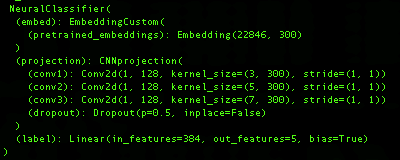
\includegraphics[scale=0.85]{pictures/fig7_static_dl_model_cnn.png}
  \caption{\textit{Static Language Model Classifier: CNN Architecture}}
  \label{fig7}
\end{figure}

The custom embedding layer combines pretrained embeddings with learnable embeddings, and optionally WCEs, to allow the model to be tailored specifically for the dataset in question that is fed into the model for training. This representation form is what is used to initialize the embedding layer of the neural models, which again is used at runtime, i.e. at training time, to be retrieved by the classifier and processed by the neural model in question, pooled together in batches, and ultimately classified the transformation layers of the different deep learning models we test with. Once the dataset is indexed, a process which must be aligned with the tokenization strategy of the underlying language model we are working with, we then test each of the static word embedding neural classifiers under different hyperparameter settings and with each of the in scope datasets, both with and without WCEs, resulting in metrics - like the initial set of ML classifier data - that can be directed compared against the 2021 study \cite{moreo2021}. During training, these indexed, numerical representations of the documents are batched and passed to the model's embedding layer through the NeuralClassifier so that, via the EmbeddingCustom layer, the appropriate embeddings for each token from the embedding matrix (pretrained + learnable embeddings) can be retrieved and used for downstream processing. 

The embeddings are then, in the forward method of the classifier, processed by either the CNN, LSTM, or ATTN projection layers depending upon the type of neural classifier being trained, the end result of which yields a contextual, language model embedding representation of the documents is created for the underlying model. One of the primary differences between the static language models and the dynamic ones in fact, is the tokenization strategy that is used. While static word embeddings are designed to look at, and represent words\footnote{Or in the case of fastText subwords but ultimately these are words in the sense that the subwords themselves do in fact have a semantic meaning}, the transformer-based models break language down into tokens, which while solving for out of vocabulary and polysemy type problems, nonetheless moves the language representation form away from word, term or subword based semantic space, to a more granular semantic space whose dimensions are defined by the dictionary of tokens that is established and used by the language model in question.

\paragraph{Dynamic Neural Classifiers: Transformers}

The transformer model testing workflow, and data preparation, is slightly different than the neural classifier test script for the static pretrained language models. We use two distinct classifier architectures that are built off of the Hugging Face libraries - namely the SequenceClassifier and a simple CNN, neural network architecture that is modelled after the same neural architecture we use for the static language model testing. The basic test workflow is designed to generate a Classifier of a given type, with a given pretrained language model, a given underlying dataset, and a set of program and model hyperparameters that define the test run. Each run is logged with details around system parameters (OS, GPUs, CPUs, memory, etc.), language model type and attributes, the dataset and classifier type, and other hyperparameters to be used by Layer Cake Reporting \& Analytics module for analysis.

The power of this transformer-based approach, which dominates the language model research and development landscape right now for good reason, is predicated on the construction of an embedding space that is defined by the underlying tokenization dictionary used by the language model in question, as well as these models' ability to generate context-aware embeddings via the attention mechanism. This granularity with respect to the underlying semantic space yields very accurate results across a variety of NLP problems but nonetheless comes at a cost in terms of the system resource and computational requirements which are necessary to generate the kind of granularity necessary to drive the performance improvements. Much of the computational complexity around working with transformer based language models is from this runtime complexity that is driven from the computational requirements of the underlying language model itself, which clearly does a lot of work to generate the context aware embeddings, which are of course the main distinguishing characteristic of the transformer-based models versus their static counterparts. In other words, given the dynamic nature of the transformer based embeddings, the embeddings - the model really - has to sit in a different type of neural classifier entirely that accounts for, and incorporates, the underlying language model directly into the classifier so that the embeddings can be computed, dynamically, and then they can be pooled and fed to the classifier head portion of the model. One of the implications of this technical dependency is that the static based neural models are significantly less computationally intensive than their transformer-based counterparts, one of the key measurement findings of this study in fact. What's also less intuitive but nonetheless another important finding of this study is that the neural classifiers we use with the static language are also more flexible, more configurable and optimizable, and also less computationally intensive than their more sophisticated, context-aware embedding generating counterparts (i.e. transformer language models). 

We see this for example in the way the Embedding Layer is structured and how it can be configured in the static neural classifiers versus the dynamic ones - the embedding layer being the foundational structure of all of the neural model classifiers that is used to generate the embeddings that are used to represent the text of the underlying dataset, either as a straight index lookup in the forward pass of the model as is the case with the static neural models, or as inputs into the runtime computational dynamic embeddings that the transformer models generate and that can be consumed, really pooled, for classification in the forward pass of model training. Specifically, with the static (word) embedding designed neural classifiers, we have the ability to both filter as well as add on to this initialized Embedding layer, concatenating WCEs in some cases, as well as filtering out the unneeded embeddings in order to optimize the layer by only using the word embeddings that are necessary for the task at hand, rather than the entire language model embedding dictionary which is the case for transformer models. It's this flexibility that allows for WCEs to be integrated into the neural classifiers for the static word embeddings language models, but not for the transformer-based language models which, given their internal dependency on the underlying computational logic that is intrinsic to the language model type itself, cannot be extended horizontally (concatenated) with TCEs (token-class embeddings) without breaking the model.

The transformer-based classifiers are, given the dynamic nature of the underlying language models, integrated directly with the language models which are neural network models in and of themselves, each of which dictates the structure, size and content of its underlying embedding layer - i.e. the specific model data. Outside of the computational logic differences between the static and dynamic language representation forms, the other main difference between the two sets of neural classifiers is of course both the structure, and content, of this embedding layer which provides the computational basis for embedding representation by the language model for the dataset in question - for both the static language models as well as the dynamic ones. As illustrated in the CNN HF transformer classifier shown below for example, the embedding layer is initialized to include the entire dictionary of token embeddings for the bert-base-cased language model we use, a language model which has 28,996 pretrained token embeddings, each of which is of size 768, i.e. the embedding dimension size or the hidden\_size of the (language) model. The HF CNN architecture, as the name implies, leverages a CNN neural architectural approach to classification constructed directly on top of the HF transformer model itself, allowing for the transformer computed embeddings to be first pooled and then passed into the CNN for classification. The Hugging Face Sequence Classifiers are structured the same way, but each of the transformer models has its own unique classifier attached to it, not necessarily a CNN like we use as shown in the figure below, which is analogous to the CNN classifier we use for testing the static word embeddings. 

We would point out that for both of these (Hugging Face) transformer model classifiers that we use with Layer Cake, the initial embedding layer is fixed, constrained by the underlying language model itself - which in this case consists of 28,996 token embeddings, each of which is a vector of size 768 and each of which maps back to a token in the dictionary space of the specific BERT language model variant being used - bert-base-cased in our work. As mentioned previously, given the tight coupling of this embedding layer with the runtime computational requirements necessary to generate context-aware embeddings which is built into the model itself, we were not able to extend, or minimize (optimize) this initial embedding layer at all for any of the transformer models without breaking them (i.e. they become non-functional) so it's fair to say that with the extra granularity and complexity that is built into these transformer language models, comes not just state-of-the-art results, but also mandated minimal computational and resource requirements that are dictated by the model itself rather than the input data that we are using to feed into the model - in other words no matter what the use case the full model must be used. 

This lack of flexibility also shows up when we try and integrate externally trained embeddings into the model, e.g. WCEs or TCEs, which a) cannot be concatenated with the initial model embeddings in the Embedding Layer and so can only be integrated in the forward pass when the context-aware embeddings are computed, and b) are ineffective when pooled together with the run-time computed, context-aware embeddings in the forward pass of the model, no matter how they are integrated (dot product, linear transformation, addition). As we state earlier, the TCEs not only did not help the performance of the models (as measured by Macro-F1 or Micro-F1 or any performance measure for that matter), they seem to confuse the models and have a negative impact on performance, despite the fact that in theory at least, they should add additional information which helps the classification of sequence of tokens that is being pooled. This is not the case however. As one might expect, this embeddings layer, BertEmbeddings in this case, is tightly coupled with the language model, which as one can see from the neural model shown below actually makes up the bulk of the whole neural model classifier itself. It's this model integration which allows for the dynamically generated (transformer) embeddings, for the specific sequence in question, to be passed to the classifier layers of the neural model during training (the forward pass). In other words, one of the distinguishing characteristics of these transformer models is that they themselves are rigidly fixed and heavily dependent on both the size and dimension, and contents, of their embeddings. While this shouldn't come as a surprise necessarily, it should be kept in mind when one considers what kind of flexibility one needs with a language model - like for example if there are other embedding forms that one wants to use in conjunction with pretrained language model embeddings, TCEs for example.


\begin{figure}[h!]
	\centering
	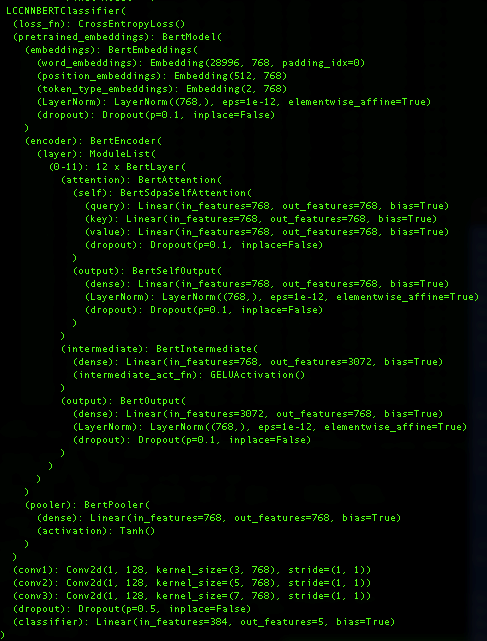
\includegraphics[scale=0.85, width=0.9\textwidth, height=15.5cm]{pictures/fig8_lc_cnn_bert_classifier.png}
	\caption{\textit{LCCNNBERTCLassifier Architecture: Hugging Face transformers}}
	\label{fig8}
\end{figure}  


Therefore, given the more rigid nature of the embedding layer for the HF transformer classifiers, they are not well suited for either a) filter optimization methods example to only include token embeddings for those in scope for a given dataset, or b) extend the feature space of the embedding layer to include embeddings trained outside the model, like for example WCEs or TCEs in the case of transformers. Both of these optimizations are available if we are hand crafting the neural classifier using static embeddings however and they are applied for this set of test data (the static embedding test data) and have a significant impact on the runtime performance, aka computational requirements, of these models. This cannot be emphasized enough how important these factors are in any cost-benefit analysis of the relative performance of classifiers and/or language models and/or representation forms, as we demonstrate in this work.

The only way in fact that we could test the relative effect of TCEs in our HF, transformer-based language model driven classifiers was by was by including the TCEs with the dynamically generated embeddings in the forward pass of training and using various combinations of these two types of embeddings into the downstream classifier parts of the neural network architecture. And what we found, quite conclusively after a wide range of approaches to integrating the TCEs with the transformer model generated embeddings was that if anything, the inclusion of TCEs into the transformer model classifiers - whether by concatenation or dot product operations, i.e. linear transformations or projections effectively\footnote{We experimented with dot product operations, addition operations, and concatenation operations of the transformer generated embedding representations of the text with the TCEs that we computed per class (per token). None of these methods worked for any of the transformer models we tested. We hypothesize that, given how well the transformer models perform generally relative to both their static embedding counterparts and the baseline ML classifiers we test with (SVMs, Logistic Regression methods primarily), that this is because the additional information that is encapsulated in these TCEs is already part of the underlying transformer model representation of the text at some level and therefore adding it to the embeddings only proves to reduce the effectiveness of the classification portion of the classifier. NB The WCEs are combined with the static language model embeddings via concatenation, i.e. we extend the embedding layer dimensions to include the WCEs yielding a richer word representation that is fed into the model during training.} - made the classifier less effective, despite the additional information that the TCEs contained. This is in fact, another one of the unique contributions of this work, i.e. that not only does adding the TCEs into transformer models prove ineffective, but that the underlying embedding layer of the transformer models does not lend itself to customization.

The final results we look at in for the transformer classifiers use a 4 A100 GPU system, distributed using the PyTorch DataParallel form of model parallelism, which is the default mode used by the HF APIs, whereas the neural models needed just one (dedicated) GPU. For the HF transformer language model script, we have two different classifiers that we use, a built in HF Sequence Classifier which encapsulates the language model specific logic for you in a custom classifier alongside a simple CNN based architecture which is modelled after the CNN neural net that we use with the static embeddings.

\section{Results \& Analysis}
In this section we analyze the data from the different Layer Cake test scripts, focusing on the primary dimensions of analysis that we are concerned with in this study, namely classifier architecture and language representation forms. We look at the ML data first, followed by the neural models, and then the summary analysis across the broad spectrum of classifiers included in Layer Cake to a get a full picture of the data. 

For the purposes of the neural model analysis, we group the static and dynamic classifier test results together, yielding a comparative perspective for this specific dimension, static versus dynamic language models, which gives us a unique perspective on a) how much better the transformers are for this particular use case (classification) and b) what the underlying cost is computationally for this improvement. This puts us in a unique position to be able to ascertain the cost, again computationally, for the step up in model improvement - a measure we have not seen in the literature before. For the ML classifiers, our baseline testing module effectively, we look at the several different dimensions of the results data, evaluating performance across the classifiers, the representation forms and the language model types.\footnote{Note that all of the data we look at for the ML classifiers was generated with the default parameters, to get the breadth and scope of the hyperparameter and representation forms for the different variations of classifiers and language types, optimized runs proved very time consuming, particularly the LR classifiers for the larger datasets (RCV), and language models (Llama).} 


\subsection{ML Classifier Testing: Baselines}

We look at the baseline ML results by Classifier, Dataset and Representation Form, with each dimensional analysis supported by visualizations and summary data generated by Layer Cake's Reporting and Analytics module, developed in Python using seaborn, matplotlib, tabulate, and bokeh libraries for visualization.\footnote{See https://seaborn.pydata.org/, https://matplotlib.org/, https://pypi.org/project/tabulate/, https://bokeh.org/ respectively.}


\subsubsection{By ML Classifier}

Layer Cake supports three different types of classical ML classifiers - Support Vector Machines (SVM), Logistic Regression (LR), and Naive Bayes (NB) - each of which has proven to be effective for the classification of text (see Research Context section above for details). To visualize the results by classifier SVM, we use a box-and-whisker plot. In Figure \ref{fig9} (below) we present the Macro-F1 results above the Micro-F1 results. This box plot shows the data distribution based on a five-number summary: minimum, first quartile (Q1), median, third quartile (Q3), and maximum which helps show the central tendency of the underlying data as well as the data spread and outliers. The 'box', which is the shaded area (from Q1 to Q3) represents the interquartile range (IQR), which is the range between the first quartile (Q1) and the third quartile (Q3). The height of the box gives you an idea of the spread of the middle 50\% of the data, i.e. a taller box indicates more variability in the data, while a shorter box means the values are closer together. 

\begin{figure}[h!]
	\centering
	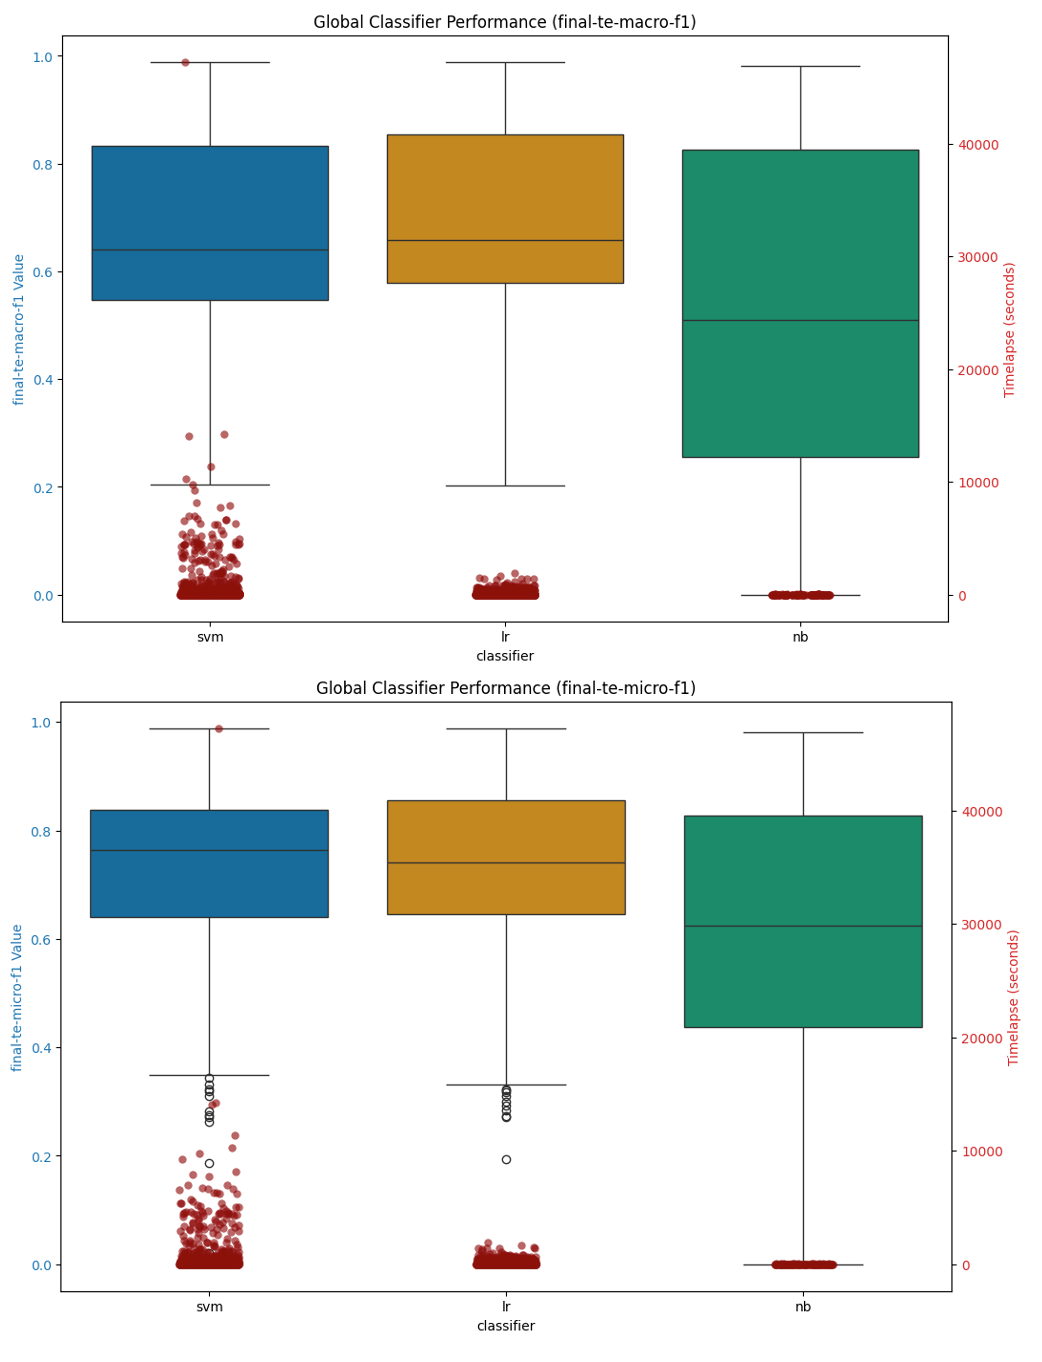
\includegraphics[width=0.9\textwidth, height=16.5cm]{pictures/fig9_ml_classifier_perf_summ.png}   
	\caption{\textit{ML Classifier Performance Summary: Macro-F1 and Micro-F1 Scores}}
	\label{fig9}
\end{figure}  

On average across the datasets and language models, the LR models perform slightly better than the SVM classifiers, and both the SVM and LR classifiers perform slightly better than the Naive Bayes models.\footnote{The Naive Bayes classifier is built using the MultinomialNB API from scikit-learn which, within the context of Layer Cake testing, only supports text vectorization forms of language representation given that it requires input data to be positive, which is not the case for LLM embeddings.} The runtimes for the classifiers are clustered below 10,000 seconds, which equates to just under three hours for model construction, with the bulk of the classifiers, particularly for the Logistic Regression models, at around 1000 seconds which is 16 minutes, very reasonable. The SVM classifier models take slightly more time to build which is expected given the computational complexity of the underlying mathematics for SVMs versus their LR or NB counterparts. Naive Bayes is the most efficient of the models but given the nature of the model does not support negative numbers and as such can only be used with text vectorization representation forms, most embeddings spill into negative dimensional space, but generally speaking the metrics hold up for NB as well.

When we look at the top 5 Classifier Macro \& Micro F1 scores by Dataset and Representation form, as illustrated in Table \ref{tab:ml_classifier_summary_macro_f1} and Table \ref{tab:ml_classifier_summary_micro_f1} below, we can see that both the SVM and LR Classifiers both perform comparatively well, and that generally the text vectorization techniques (TF-IDF or Count) dominate the best results, with some limited exceptions. 

\begin{table}[h!]
\centering
\scriptsize
\caption{ML Classifier Performance Summary - Macro-F1 Top 5 Values}
\label{tab:ml_classifier_summary_macro_f1}
\begin{tabular}{@{}p{.7cm} p{1.8cm} c >{\raggedright\arraybackslash}p{6.1cm} r p{1.0cm}@{}}
\toprule
\textbf{Clf} & \textbf{Dataset} & \textbf{Dims} & \textbf{Representation} & \textbf{Value} & \textbf{Time} \\
\midrule
svm & 20newsgroups & (11314, 22920) & count+llama(avg):def & 0.705 & 64.75 \\
lr & 20newsgroups & (11314, 24988) & tfidf+tfidf.(llama+wce(tfidf))+tfidf.(llama+wce(tfidf)):def & 0.703 & 314.08 \\
lr & 20newsgroups & (11314, 4116) & llama(avg)+tfidf.(llama+wce(tfidf)):def & 0.701 & 36.34 \\
lr & 20newsgroups & (11314, 22920) & count+llama(avg):def & 0.700 & 787.88 \\
svm & 20newsgroups & (11314, 4116) & llama(avg)+tfidf.(llama+wce(tfidf)):def & 0.689 & 133.89 \\
\midrule
lr & arxiv & (11962, 18997) & count+llama(avg):def & 0.784 & 466.42 \\
svm & arxiv & (11962, 18997) & count+llama(avg):def & 0.776 & 59.19 \\
lr & arxiv & (11962, 18948) & tfidf+llama(avg):def & 0.769 & 151.81 \\
lr & arxiv & (11962, 2048) & llama(avg):def & 0.769 & 22.03 \\
svm & arxiv & (11962, 18948) & tfidf+llama(avg):def & 0.765 & 23.97 \\
\midrule
lr & arxiv\_protoformer & (82500, 34540) & tfidf+llama(avg):def & 0.857 & 2569.18 \\
lr & arxiv\_protoformer & (82500, 2048) & llama(avg):def & 0.856 & 184.94 \\
lr & arxiv\_protoformer & (82500, 1536) & deepseek(avg):def & 0.855 & 154.60 \\
svm & arxiv\_protoformer & (82500, 1536) & deepseek(avg):def & 0.850 & 238.68 \\
svm & arxiv\_protoformer & (82500, 32930) & tfidf+deepseek(avg):def & 0.850 & 1571.72 \\
\midrule
lr & bbc-news & (1229, 1541) & xlnet(avg)+tfidf.(xlnet+wce(tfidf)):def & 0.989 & 2.34 \\
lr & bbc-news & (1229, 8969) & tfidf+tfidf.(xlnet+wce(tfidf))+tfidf.(xlnet+wce(tfidf)):def & 0.989 & 3.47 \\
lr & bbc-news & (1229, 1541) & roberta(avg)+tfidf.(roberta+wce(tfidf)):def & 0.989 & 1.86 \\
lr & bbc-news & (1229, 8537) & tfidf+tfidf.(roberta+wce(tfidf))+tfidf.(roberta+wce(tfidf)):def & 0.989 & 1.72 \\
svm & bbc-news & (1229, 768) & gpt2(avg):def & 0.988 & 1.72 \\
\midrule
lr & imdb & (25000, 30664) & tfidf+roberta(avg):def & 0.925 & 198.31 \\
lr & imdb & (25000, 2048) & llama(avg):def & 0.923 & 27.83 \\
svm & imdb & (25000, 768) & roberta(avg):def & 0.922 & 9.38 \\
lr & imdb & (25000, 32714) & tfidf+llama(avg):def & 0.921 & 489.62 \\
lr & imdb & (25000, 768) & roberta(avg):def & 0.921 & 7.65 \\
\midrule
svm & ohsumed & (24061, 18940) & tfidf fasttext:def & 0.691 & 13.22 \\
svm & ohsumed & (24061, 18940) & tfidf glove:def & 0.691 & 13.44 \\
svm & ohsumed & (24061, 18940) & tfidf word2vec:def & 0.691 & 14.11 \\
svm & ohsumed & (24061, 19240) & tfidf+fasttext(avg):def & 0.690 & 20.48 \\
svm & ohsumed & (24061, 19240) & tfidf+word2vec(avg):def & 0.687 & 17.97 \\
\midrule
lr & rcv1 & (23149, 30931) & count+llama(avg):def & 0.648 & 11126.84 \\
lr & rcv1 & (23149, 30931) & tfidf+llama(avg):def & 0.635 & 8408.93 \\
lr & rcv1 & (23149, 2048) & llama(avg):def & 0.633 & 889.43 \\
svm & rcv1 & (23149, 28679) & tfidf+roberta(avg):def & 0.629 & 5519.30 \\
svm & rcv1 & (23149, 2048) & llama(avg):def & 0.624 & 1749.58 \\
\midrule
svm & reuters21578 & (9603, 9556) & tfidf+glove(avg):def & 0.606 & 19.01 \\
svm & reuters21578 & (9603, 9556) & tfidf+fasttext(avg):def & 0.606 & 16.72 \\
lr & reuters21578 & (9603, 9256) & tfidf fasttext:def & 0.600 & 19.53 \\
lr & reuters21578 & (9603, 9256) & tfidf glove:def & 0.600 & 20.87 \\
lr & reuters21578 & (9603, 9256) & tfidf word2vec:def & 0.600 & 22.29 \\
\bottomrule
\end{tabular}
\end{table}


\begin{table}[h!]
\centering
\scriptsize
\caption{ML Classifier Performance Summary - Micro-F1 Top 5 Values}
\label{tab:ml_classifier_summary_micro_f1}
\begin{tabular}{@{}p{.7cm} p{1.8cm} c >{\raggedright\arraybackslash}p{5.8cm} r p{1.0cm}@{}}
\toprule
\textbf{Clf} & \textbf{Dataset} & \textbf{Dims} & \textbf{Representation} & \textbf{Value} & \textbf{Time} \\
\midrule
lr & 20newsgroups & (11314, 24988) & tfidf+tfidf.(llama+wce(tfidf))+tfidf.(llama+wce(tfidf)) & 0.715 & 314.08 \\
lr & 20newsgroups & (11314, 4116) & llama(avg)+tfidf.(llama+wce(tfidf)) & 0.713 & 36.34 \\
lr & 20newsgroups & (11314, 22920) & count+llama(avg) & 0.711 & 787.88 \\
svm & 20newsgroups & (11314, 22920) & count+llama(avg) & 0.711 & 64.75 \\
svm & 20newsgroups & (11314, 4116) & llama(avg)+tfidf.(llama+wce(tfidf)) & 0.702 & 133.89 \\
\midrule
lr & arxiv & (11962, 18997) & count+llama(avg) & 0.785 & 466.42 \\
svm & arxiv & (11962, 18997) & count+llama(avg) & 0.783 & 59.19 \\
lr & arxiv & (11962, 18948) & tfidf+llama(avg) & 0.768 & 151.81 \\
svm & arxiv & (11962, 18948) & tfidf+llama(avg) & 0.765 & 23.97 \\
lr & arxiv & (11962, 21054) & tfidf+tfidf.(llama+wce(tfidf))+tfidf.(llama+wce(tfidf)) & 0.764 & 366.72 \\
\midrule
lr & arxiv\_protoformer & (82500, 34540) & tfidf+llama(avg) & 0.857 & 2569.18 \\
lr & arxiv\_protoformer & (82500, 2048) & llama(avg) & 0.856 & 184.94 \\
lr & arxiv\_protoformer & (82500, 1536) & deepseek(avg) & 0.855 & 154.60 \\
svm & arxiv\_protoformer & (82500, 1536) & deepseek(avg) & 0.850 & 238.68 \\
svm & arxiv\_protoformer & (82500, 32930) & tfidf+deepseek(avg) & 0.850 & 1571.72 \\
\midrule
svm & bbc-news & (1229, 6358) & tfidf[fasttext] & 0.989 & 0.86 \\
svm & bbc-news & (1229, 6358) & tfidf[glove] & 0.989 & 0.85 \\
svm & bbc-news & (1229, 6358) & tfidf[word2vec] & 0.989 & 0.88 \\
svm & bbc-news & (1229, 768) & gpt2(avg) & 0.989 & 1.72 \\
svm & bbc-news & (1229, 768) & tfidf->LSA[bert].(bert) & 0.989 & 3.29 \\
\midrule
lr & imdb & (25000, 30664) & tfidf+roberta(avg) & 0.925 & 198.31 \\
lr & imdb & (25000, 2048) & llama(avg) & 0.923 & 27.83 \\
svm & imdb & (25000, 768) & roberta(avg) & 0.922 & 9.38 \\
lr & imdb & (25000, 32714) & tfidf+llama(avg) & 0.921 & 489.62 \\
lr & imdb & (25000, 768) & roberta(avg) & 0.921 & 7.65 \\
\midrule
svm & ohsumed & (24061, 18940) & tfidf[fasttext] & 0.706 & 13.22 \\
svm & ohsumed & (24061, 18940) & tfidf[glove] & 0.706 & 13.44 \\
svm & ohsumed & (24061, 18940) & tfidf[word2vec] & 0.706 & 14.11 \\
svm & ohsumed & (24061, 19240) & tfidf+fasttext(avg) & 0.704 & 20.48 \\
svm & ohsumed & (24061, 19240) & tfidf+word2vec(avg) & 0.703 & 17.97 \\
\midrule
svm & rcv1 & (23149, 28679) & tfidf+roberta(avg) & 0.826 & 5519.30 \\
lr & rcv1 & (23149, 30931) & count+llama(avg) & 0.819 & 11126.84 \\
svm & rcv1 & (23149, 26758) & tfidf+word2vec(avg) & 0.816 & 4421.36 \\
svm & rcv1 & (23149, 26758) & tfidf+fasttext(avg) & 0.815 & 4174.40 \\
svm & rcv1 & (23149, 26758) & tfidf+glove(avg) & 0.812 & 4257.52 \\
\midrule
svm & reuters21578 & (9603, 9556) & tfidf+word2vec(avg) & 0.878 & 15.78 \\
svm & reuters21578 & (9603, 9556) & tfidf+fasttext(avg) & 0.877 & 16.72 \\
svm & reuters21578 & (9603, 9256) & tfidf[fasttext] & 0.877 & 5.63 \\
svm & reuters21578 & (9603, 9256) & tfidf[glove] & 0.877 & 5.82 \\
svm & reuters21578 & (9603, 9256) & tfidf[word2vec] & 0.877 & 5.77 \\
\bottomrule
\end{tabular}
\end{table}


We can also see that the model build times (the \textit{timelapse} column) are very much a function of the size of the feature matrix that is used with the model (the \textit{dimensions} column), which is what we would expect and aligns with the dimensionality complexity challenges that are fundamental to ML (our so-called \textit{curse of dimensionality}) - hence the emphasis on feature reduction techniques in the literature which have historically been shown to have a significant (positive) impact on computational resource requirements, i.e. model training times, while still retaining the bulk of their predictive power \cite{zebari2020ACR} \cite{vandermaaten2009dimensionality}. 


\subsubsection{By Representation Form}

When we look at the various representation forms that we use with the ML classifiers, as illustrated in Figures \ref{fig:fig10} and \ref{fig:fig11}, we find that - perhaps surprisingly - the \textit{lsa} and \textit{solo} representation forms (with again \textit{solo} being the representation of the underlying dataset encoded and pooled using the language model in question), both individually and when combined (concatenated) with the WCEs, are the best performing options in terms of model efficacy. Again these scores are averaged and summarized by Classifier and include data across all of the different datasets. It is also worth noting that the \textit{lsa} representation form, one of the most tried and true forms of feature reduction in NLP, is very efficient in terms of model construction times (\textit{timelapse} value) while still quite competitive in terms of Macro-F1 and Micro-F1 scores.

\begin{figure}[h!]
	\centering
	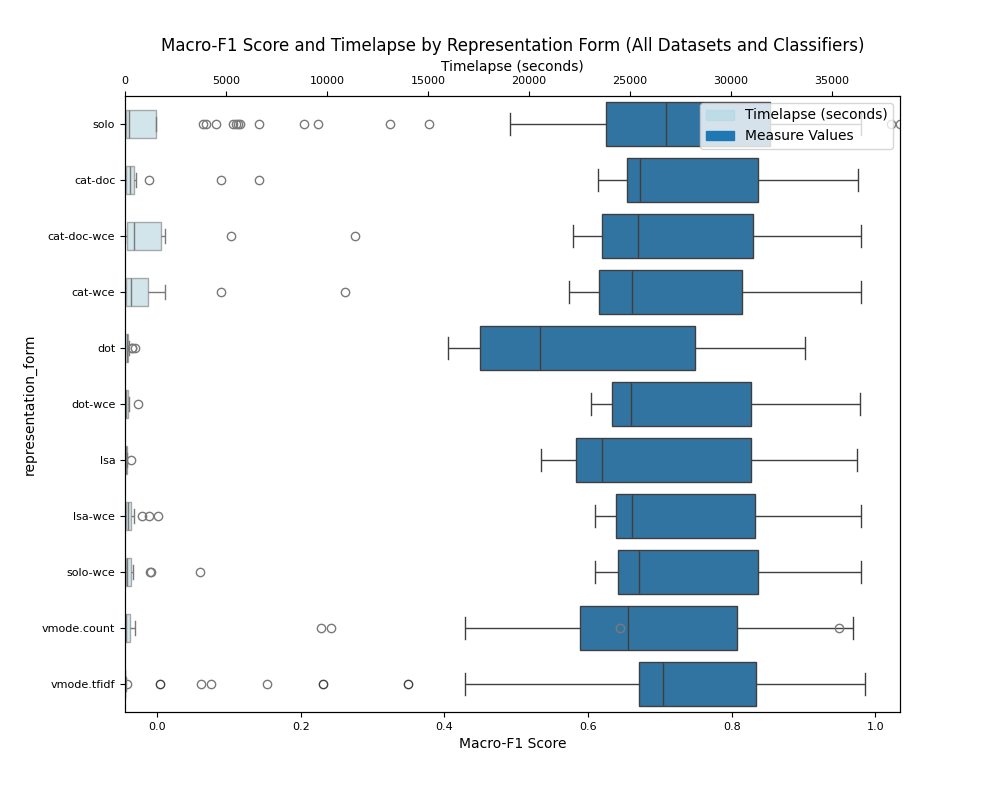
\includegraphics[width=1\textwidth, height=12.5cm]{pictures/fig10_ml_classifier_rep_form_macro_f1.png}
	\caption{\textit{ML Classifier Representation Form Results: Macro-F1}}
	\label{fig:fig10}
\end{figure}

\begin{figure}[h!]
	\centering
	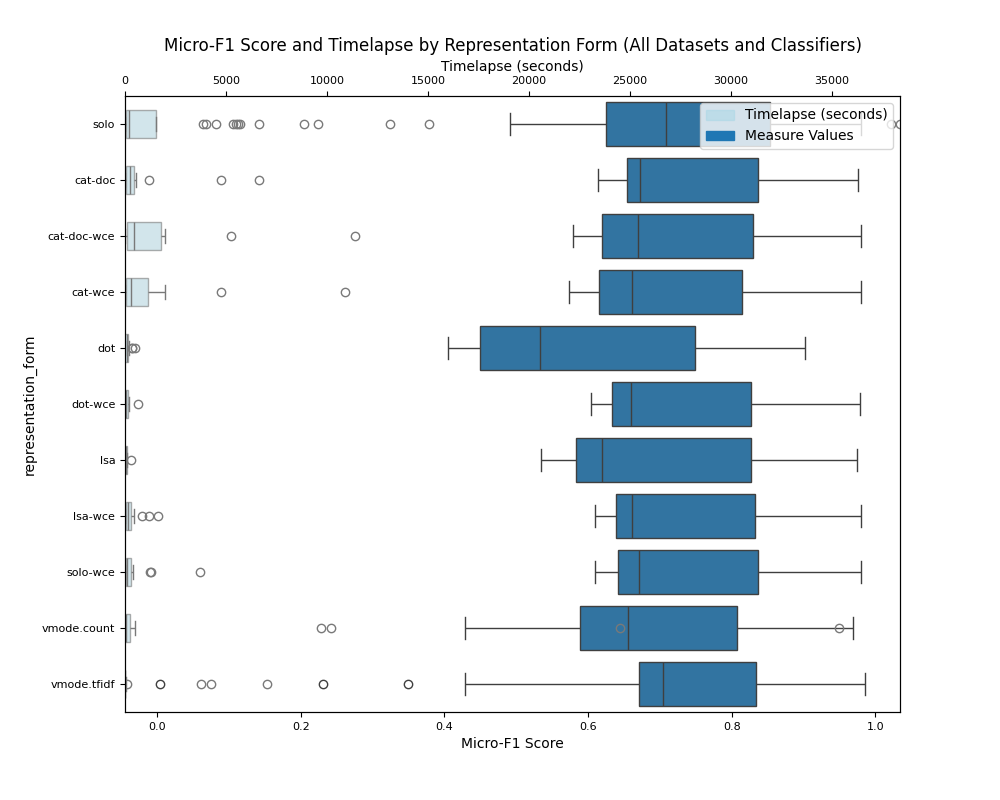
\includegraphics[width=1\textwidth, height=12.5cm]{pictures/fig11_ml_classifier_rep_form_micro_f1.png}  
	\caption{\textit{ML Classifier Representation Form Results: Micro-F1}}
	\label{fig:fig11}
\end{figure}

In looking at the breakout of representation form by dataset, as shown in Tables \ref{tab:macro_f1_repr_form} \ref{tab:micro_f1_repr_form} below, we can see that \textit{solo-wce} and \textit{lsa-wce}, along with simply \textit{solo} and \textit{wce}, perform quite well relative to the alternative forms of representation we test with. In particular when we look at the largest datasets (RCV1-V2 for example), we see \textit{solo} representation forms, which again are a form of feature reduction technique in that they are computed by encoding the dataset in question using the different language models and as such the number of features is equivalent to the vector size of the different language models (e.g. 300 for the static embedding models such as Word2Vec, GloVe and FastText and 768 for the majority of the LLMs). We can see in our results summaries that this form of language representation stands up quite well relative to the best performing forms (which are predicated on text vectorization techniques which use a much bigger feature matrix as input into the model) and yet take just a fraction of the model construction times, representing a significant computational cost savings.

For the RCV1-V2 dataset, the largest dataset we test with (news data), the Macro-F1 scores for the \textit{cat-doc} representation form which is the vectorized text combined (concatenated) with the embedding representation of the dataset (pooled embeddings), we have a value of .648 versus the .633 for \textit{solo} whereas the mean model construction time is only 392.63 seconds versus the 5686.60 seconds for the \textit{cat-doc} model, almost 15x the run time basically - 6.5 minutes versus almost an hour and a half which is a significant difference, especially if you are constantly updating your model. For the arxiv\_protoformer dataset, the best value for Macro-F1 is also \textit{cat-doc}, where we get a max value of .857 versus the .856 for \textit{solo}, whereas the mean model construction time is only 77.7 seconds, versus the 887 seconds (almost 15 minutes), again almost a 15x computational cost hit for model construction times.

\begin{table}[h!]
\centering
\scriptsize
\caption{ML Macro-F1 Performance by Representation Form}
\label{tab:macro_f1_repr_form}
\begin{tabular}{@{}p{2.2cm} p{2.6cm} c c c c c@{}}
\toprule
\textbf{Dataset} & \textbf{Representation Form} & \textbf{Mean} & \textbf{Max} & \textbf{Std Dev} & \textbf{Count} & \textbf{Timelapse} \\
\midrule
\textbf{20newsgroups} & cat-doc & 0.630 & 0.705 & 0.064 & 36 & 130.05 \\
 & cat-doc-wce & 0.619 & 0.703 & 0.105 & 36 & 258.76 \\
 & solo-wce & 0.647 & 0.701 & 0.021 & 40 & 62.59 \\
 & solo & 0.609 & 0.684 & 0.044 & 20 & 33.80 \\
 & cat-wce & 0.618 & 0.681 & 0.074 & 40 & 140.84 \\
\midrule
\textbf{arxiv} & cat-doc & 0.660 & 0.784 & 0.098 & 36 & 155.20 \\
 & solo & 0.541 & 0.769 & 0.126 & 20 & 37.39 \\
 & solo-wce & 0.664 & 0.759 & 0.034 & 40 & 99.21 \\
 & cat-doc-wce & 0.636 & 0.757 & 0.115 & 36 & 435.75 \\
 & vmode.tfidf & 0.470 & 0.741 & 0.336 & 30 & 12.45 \\
\midrule
\textbf{arxiv\_protoformer} & cat-doc & 0.818 & 0.857 & 0.024 & 38 & 827.66 \\
 & solo & 0.796 & 0.856 & 0.032 & 20 & 77.77 \\
 & cat-doc-wce & 0.822 & 0.846 & 0.017 & 37 & 1951.57 \\
 & solo-wce & 0.828 & 0.845 & 0.006 & 39 & 1966.91 \\
 & cat-wce & 0.818 & 0.840 & 0.016 & 37 & 1618.24 \\
\midrule
\textbf{bbc-news} & cat-doc-wce & 0.958 & 0.989 & 0.107 & 36 & 2.47 \\
 & solo-wce & 0.960 & 0.989 & 0.112 & 40 & 3.06 \\
 & lsa & 0.973 & 0.988 & 0.011 & 40 & 4.77 \\
 & solo & 0.975 & 0.988 & 0.007 & 20 & 2.23 \\
 & vmode.tfidf & 0.978 & 0.988 & 0.009 & 30 & 1.18 \\
\midrule
\textbf{imdb} & cat-doc & 0.884 & 0.925 & 0.024 & 40 & 156.40 \\
 & solo & 0.888 & 0.923 & 0.026 & 20 & 13.47 \\
 & cat-doc-wce & 0.844 & 0.897 & 0.056 & 40 & 247.18 \\
 & solo-wce & 0.862 & 0.896 & 0.016 & 40 & 123.66 \\
 & lsa & 0.872 & 0.889 & 0.010 & 40 & 33.94 \\
\midrule
\textbf{ohsumed} & vmode.tfidf & 0.494 & 0.691 & 0.254 & 30 & 16.44 \\
 & cat-doc & 0.618 & 0.690 & 0.038 & 40 & 367.95 \\
 & cat-doc-wce & 0.619 & 0.671 & 0.027 & 40 & 1166.05 \\
 & cat-wce & 0.616 & 0.671 & 0.031 & 40 & 806.73 \\
 & lsa-wce & 0.602 & 0.656 & 0.026 & 40 & 453.72 \\
\midrule
\textbf{rcv1} & cat-doc & 0.565 & 0.648 & 0.055 & 36 & 5686.60 \\
 & solo & 0.503 & 0.633 & 0.070 & 18 & 392.63 \\
 & vmode.tfidf & 0.431 & 0.604 & 0.226 & 27 & 5006.67 \\
 & vmode.count & 0.463 & 0.591 & 0.113 & 27 & 14796.16 \\
 & lsa & 0.489 & 0.586 & 0.048 & 36 & 203.08 \\
\midrule
\textbf{reuters21578} & cat-doc & 0.530 & 0.606 & 0.063 & 36 & 106.87 \\
 & vmode.tfidf & 0.468 & 0.600 & 0.160 & 30 & 13.09 \\
 & cat-doc-wce & 0.500 & 0.587 & 0.069 & 36 & 218.73 \\
 & solo-wce & 0.528 & 0.584 & 0.022 & 40 & 138.81 \\
 & vmode.count & 0.461 & 0.583 & 0.121 & 30 & 71.16 \\
\bottomrule
\end{tabular}
\end{table}

For the Micro-F1 scores, we see a similar pattern. The best performers are again the text vectorized representations, cat-doc which for RCV-1 dataset is .826, whereas the solo representation form is .800, only off by a small fraction of a percentage point and the runtime for the model construction is 5686 seconds for cat-doc and only 392 seconds for the solo representation form, again almost a 15x run-time performance hit for the model construction. Similarly, with the arxiv\_protoformer dataset, the Micro-F1 best score for cat-doc, which again represents the max score for the model, is .857 as compared to .856 for the solo representation form, almost the same. The runtimes for the model construction are 887 seconds for the cat-doc representation form as compared to just 77 for the solo representation, approximate 11x the build time. Clearly this points to the language models as being capable of performing quite well as a form of feature reduction, at least with respect to text classification for machine learning classifiers.

\begin{table}[h!]
\centering
\scriptsize
\caption{ML Micro-F1 Performance by Representation Form}
\label{tab:micro_f1_repr_form}
\begin{tabular}{@{}p{2.2cm} p{2.6cm} c c c c c@{}}
\toprule
\textbf{Dataset} & \textbf{Representation Form} & \textbf{Mean} & \textbf{Max} & \textbf{Std Dev} & \textbf{Count} & \textbf{Time} \\
\midrule
\textbf{20newsgroups} & cat-doc-wce & 0.627 & 0.715 & 0.105 & 36 & 258.76 \\
 & solo-wce & 0.656 & 0.713 & 0.023 & 40 & 62.59 \\
 & cat-doc & 0.638 & 0.711 & 0.073 & 36 & 130.05 \\
 & lsa-wce & 0.653 & 0.693 & 0.021 & 40 & 73.99 \\
 & solo & 0.617 & 0.693 & 0.046 & 20 & 33.80 \\
\midrule
\textbf{arxiv} & cat-doc & 0.659 & 0.785 & 0.110 & 36 & 155.20 \\
 & cat-doc-wce & 0.642 & 0.764 & 0.115 & 36 & 435.75 \\
 & solo & 0.522 & 0.763 & 0.134 & 20 & 37.39 \\
 & solo-wce & 0.669 & 0.761 & 0.034 & 40 & 99.21 \\
 & vmode.tfidf & 0.469 & 0.745 & 0.335 & 30 & 12.45 \\
\midrule
\textbf{arxiv\_protoformer} & cat-doc & 0.818 & 0.857 & 0.024 & 38 & 827.66 \\
 & solo & 0.796 & 0.856 & 0.032 & 20 & 77.77 \\
 & cat-doc-wce & 0.822 & 0.845 & 0.017 & 37 & 1951.57 \\
 & solo-wce & 0.829 & 0.844 & 0.006 & 39 & 1966.91 \\
 & cat-wce & 0.818 & 0.841 & 0.016 & 37 & 1618.24 \\
\midrule
\textbf{bbc-news} & cat-doc-wce & 0.959 & 0.989 & 0.103 & 36 & 2.47 \\
 & lsa & 0.974 & 0.989 & 0.011 & 40 & 4.77 \\
 & solo & 0.976 & 0.989 & 0.007 & 20 & 2.23 \\
 & solo-wce & 0.961 & 0.989 & 0.104 & 40 & 3.06 \\
 & vmode.tfidf & 0.978 & 0.989 & 0.010 & 30 & 1.18 \\
\midrule
\textbf{imdb} & cat-doc & 0.884 & 0.925 & 0.024 & 40 & 156.40 \\
 & solo & 0.888 & 0.923 & 0.026 & 20 & 13.47 \\
 & cat-doc-wce & 0.846 & 0.897 & 0.048 & 40 & 247.18 \\
 & solo-wce & 0.863 & 0.896 & 0.016 & 40 & 123.66 \\
 & lsa & 0.872 & 0.889 & 0.010 & 40 & 33.94 \\
\midrule
\textbf{ohsumed} & vmode.tfidf & 0.567 & 0.706 & 0.178 & 30 & 16.44 \\
 & cat-doc & 0.645 & 0.704 & 0.031 & 40 & 367.95 \\
 & cat-wce & 0.643 & 0.691 & 0.027 & 40 & 806.73 \\
 & cat-doc-wce & 0.644 & 0.690 & 0.025 & 40 & 1166.05 \\
 & lsa-wce & 0.635 & 0.676 & 0.023 & 40 & 453.72 \\
\midrule
\textbf{rcv1} & cat-doc & 0.772 & 0.826 & 0.034 & 36 & 5686.60 \\
 & vmode.tfidf & 0.722 & 0.812 & 0.103 & 27 & 5006.67 \\
 & solo & 0.686 & 0.800 & 0.062 & 18 & 392.63 \\
 & lsa & 0.696 & 0.792 & 0.042 & 36 & 203.08 \\
 & cat-doc-wce & 0.744 & 0.790 & 0.051 & 36 & 8329.86 \\
\midrule
\textbf{reuters21578} & cat-doc & 0.814 & 0.878 & 0.088 & 36 & 106.87 \\
 & vmode.tfidf & 0.774 & 0.877 & 0.119 & 30 & 13.09 \\
 & lsa & 0.803 & 0.861 & 0.041 & 40 & 50.43 \\
 & cat-doc-wce & 0.778 & 0.859 & 0.114 & 36 & 218.73 \\
 & solo-wce & 0.821 & 0.859 & 0.013 & 40 & 138.81 \\
\bottomrule
\end{tabular}
\end{table}



\subsection{Neural Classifiers (Deep Learning)}

Within the context of our neural classifier model analysis, we look at performance results by classifier and by (pretrained) language models and integrate the results with model training times (timelapse field) into one graphic, focusing on the macro-f1 and micro-F1 metrics which are good, industry standard metrics to measure the performance of a classifier in both multi-label and single-label scenarios\footnote{Specific formulas for metric calculation can be found in the Experimental Setup section of this work.}.  

The primary questions we are looking at answering here are:
\begin{enumerate}
	\setlength{\itemsep}{0pt}
  	\setlength{\parskip}{0pt}
    \item \textit{pretrained embedding performance comparison}: which pretrained language models perform the best and by how much? Do certain pretrained embeddings perform better on certain datasets? If so why? If not why not?
    \item 	\textit{neural architecture performance comparison}: which neural architectures perform the best in terms of model macro-f1 and micro-f1 metrics? Is this the same across all datasets or does it differ?
    \item \textit{system resource performance comparison}: what are the computational resource requirements required to train each classifier, i.e. how many GPUs are required, and for how long, to fine-tune each model with each dataset? What is the most effective model that takes the minimal amount of computing resources to train while still retaining competitive results?
\end{enumerate}


\subsubsection{By Language Model} 

When looking at the on average best performing language models, of the model variants that we have chosen for this work, we find that XLNet and RoBERTa stand out as top performers, with the transformer models outperforming their static counterparts, even when they were assisted with WCEs, again on average. We can see this illustrated in the language model summary macro-f1 and micro-f1 charts (box plots) below. With the box plot graphic, which looks at the left y-axis which shows the measurement value between 0 and 100 (\%), with the center line representing the median value, the shaded box area the interquartile range between the 25th and 75th percentiles, and outliers represented as unshaded circles. Overlaid on these graphics is the timelapse value which shows how it took, in seconds, to build (train) the model.

We also see, again on average across all the datasets, relatively the same performance for the three static word embedding language models we test with (GloVe, Word2Vec and fastText models). Given that they are of comparable size and are trained basically on the same underlying data (Web Common Crawl), this is not a surprising result and speaks to how comparable the different training methods are to each other when used in this type of neural model / text classification setting. We see the best performance across all the datasets that we tested from the XLNet and RoBERTa language models, with BERT, GPT2 and DeepSeek coming in very close behind those two frontrunners. 

\begin{figure}[h!]
	\centering
	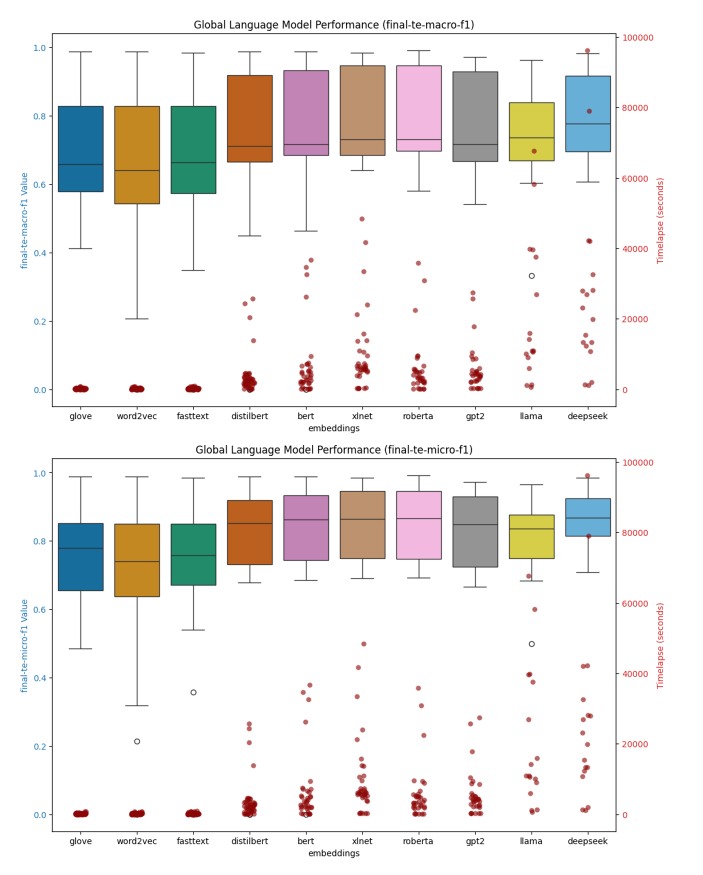
\includegraphics[width=1\textwidth, height=14.5cm]{pictures/fig12_neural_classifier_lang_model_perf_summ.png} 
	\caption{\textit{Neural Classifier Language Model Type Performance Summary}}
	\label{fig12}
\end{figure}

Notably however, from a computational resource requirements perspective (the timelapse, secondary y-axis data on the right), the static models are significantly cheaper to build. According to our analysis, the computational resource requirements of the transformer models are 50x those of their static counterparts, and this does not take into account the 4 to 1 GPU ratio that the model training of the transformers used. This accounts for some 200x more computational resources required by the transformer model training versus the static model in our analysis. 

Also, it's also important to understand that this computational costs is not just a one-time cost, in the event that you want your model to be updated on an ongoing basis, which is the case in any operational setting, that represents a 50x incremental resource cost for each and every model training update on an ongoing basis which, over time, geometrically expands the gap resource wise between what would be required to train a static embedding model versus a transformer, dynamic model.


\begin{table}[h!]
\centering
\small
\caption{Average Training Time by Model Type}
\label{tab}
\begin{tabular}{lrr}
\toprule
\textbf{Model Type} & \textbf{Avg Training Time (seconds)} & \textbf{Average Training Time (minutes)} \\
\midrule
Static & 182.8344083 & 3.047240138 \\
Transformer & 9978.987402 & 166.3164567 \\
\midrule
& \textbf{Training time Factor:} & \textbf{54.5793732} \\
\bottomrule
\end{tabular}
\end{table}


\subsubsection{By Classifier}

When we look at the data in aggregate by Classifier as shown in Figure \ref{fig:fig13}, we see the same trend from another perspective - namely that the Hugging Face transformer classifiers perform better than their static counterparts, but their training cost is significantly higher.

\begin{figure}[h!]
	\centering
	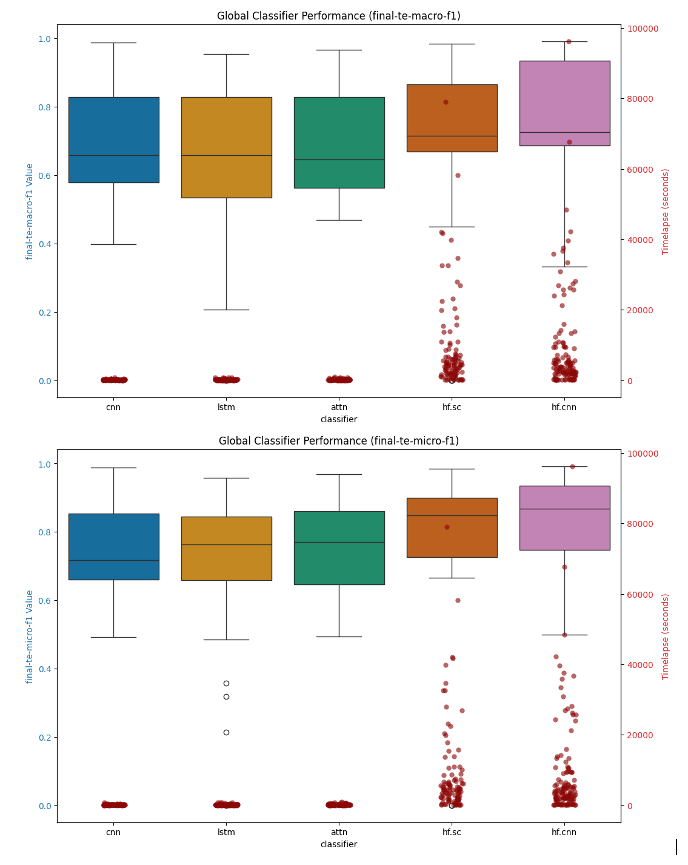
\includegraphics[width=1\textwidth, height=12.5cm]{pictures/fig13_neural_model_classifier_perf_summ.png}   
	\caption{\textit{Neural Model Classifier Performance Summary}}
	\label{fig:fig13}
\end{figure}

When we look at the detail, as illustrated in Table \ref{tab:neural_training_times}, we can see that while on average we get a .042 and .077\% increase in effectiveness of the transformer models and classifiers for Macro-F1 scores, and a .049 and .091\% increase in effectiveness for Micro-F1 scores for the transformer models over the best performing static language model neural classifiers (CNN), we nonetheless find that it takes approximately 200x the elapsed time to train the underlying (transformer) classifiers.\footnote{The 200x figure comes from the fact that it takes around 50x the time to train the models but the (transformer) models were trained on 4 GPUs while the static models on just a single GPU.} 


\begin{table}[h!]
\centering
\footnotesize
\caption{Neural Classifier Avg Training Times by Classifier}
\label{tab:neural_training_times}
\begin{tabular}{llrrr r} % last column now right-aligned
\toprule
\textbf{Classifier} & \textbf{Measure} & \textbf{Mean} & \textbf{Median} & \textbf{Count} & \textbf{Timelapse} \\
\midrule
lstm    & final-te-macro-f1 & 0.664 & 0.658 &  99 &  186.14 \\
attn    & final-te-macro-f1 & 0.691 & 0.646 & 104 &  197.00 \\
cnn     & final-te-macro-f1 & 0.700 & 0.659 & 100 &  164.84 \\
hf.sc   & final-te-macro-f1 & 0.742 & 0.715 & 101 & 8797.42 \\
hf.cnn  & final-te-macro-f1 & \textbf{0.777} & 0.726 & 124 & 9044.06 \\
\midrule
lstm    & final-te-micro-f1 & 0.727 & 0.763 &  99 &  186.14 \\
attn    & final-te-micro-f1 & 0.752 & 0.771 & 104 &  197.00 \\
cnn     & final-te-micro-f1 & 0.759 & 0.716 & 100 &  164.84 \\
hf.sc   & final-te-micro-f1 & 0.807 & 0.848 & 101 & 8797.42 \\
hf.cnn  & final-te-micro-f1 & \textbf{0.849} & 0.867 & 124 & 9044.06 \\
\bottomrule
\end{tabular}
\end{table}


That's the difference between \textit{2-3 minutes} - which is how long on average it takes to build the static, lightweight PyTorch classifiers designed to work with the precomputed, static, language model embeddings - versus \textit{2.5 hours} it takes to build the Hugging Face transformer models.\footnote{These training times are averaged across all datasets and all classifiers.} Now while certainly there is room for improvement with respect to how we optimized the training for our transformer models, this is nonetheless a staggering difference in compute resource requirements to train the different types of classifiers, with a heavy price to pay (literally and figuratively) for the performance improvement gains.

We can also see that the custom CNN classifier head that we added to the Hugging Face transformer models performs slightly better than the built in Hugging Face Sequence Classifiers, .035\% better on Macro-F1 scores and .042\% better on average for the Micro-F1 scores, illustrating that performance gains can be had by adding customized, tailored layers to the transformer models optimized for specific tasks, with the CNN based approach for classification showing surprising resilience.

\subsubsection{By Dataset}


\begin{table}[h!]
\centering
\scriptsize
\caption{Best DL Classifier Macro-F1 Performance by Dataset}
\label{tab:dl_classifier_macro_f1}
\begin{tabular}{@{}p{2cm}p{1.2cm}rrrrrrr@{}}
\toprule
\textbf{Dataset} & \textbf{Classifier} & \textbf{Max} & \textbf{Mean} & \textbf{Median} & \textbf{Min} & \textbf{Std} & \textbf{Count} & \textbf{Time} \\
\midrule
\textbf{20newsgroups} & hf.sc & 0.706 & 0.683 & 0.684 & 0.663 & 0.012 & 13 & 3843.29 \\
 & hf.cnn & 0.704 & 0.690 & 0.688 & 0.674 & 0.009 & 13 & 3986.35 \\
 & cnn & 0.694 & 0.672 & 0.674 & 0.649 & 0.014 & 12 & 115.84 \\
 & lstm & 0.681 & 0.640 & 0.642 & 0.590 & 0.030 & 12 & 56.35 \\
 & attn & 0.676 & 0.646 & 0.642 & 0.612 & 0.021 & 12 & 54.03 \\
\midrule
\textbf{arxiv} & hf.cnn & 0.821 & 0.731 & 0.726 & 0.708 & 0.029 & 13 & 4516.82 \\
 & hf.sc & 0.804 & 0.547 & 0.681 & 0.000 & 0.314 & 13 & 6640.57 \\
 & lstm & 0.696 & 0.499 & 0.568 & 0.000 & 0.200 & 23 & 159.15 \\
 & attn & 0.694 & 0.579 & 0.580 & 0.483 & 0.060 & 24 & 152.10 \\
 & cnn & 0.691 & 0.595 & 0.595 & 0.459 & 0.052 & 24 & 139.24 \\
\midrule
\textbf{arxiv\_protoformer} & hf.sc & 0.865 & 0.847 & 0.847 & 0.830 & 0.008 & 13 & 13097.29 \\
 & hf.cnn & 0.864 & 0.848 & 0.847 & 0.839 & 0.006 & 13 & 15057.97 \\
 & attn & 0.832 & 0.823 & 0.824 & 0.807 & 0.007 & 12 & 363.89 \\
 & cnn & 0.828 & 0.804 & 0.807 & 0.764 & 0.019 & 12 & 276.43 \\
 & lstm & 0.828 & 0.822 & 0.824 & 0.804 & 0.007 & 11 & 329.44 \\
\midrule
\textbf{bbc-news} & hf.cnn & 0.992 & 0.973 & 0.972 & 0.955 & 0.010 & 25 & 372.04 \\
 & cnn & 0.988 & 0.979 & 0.982 & 0.959 & 0.009 & 12 & 7.68 \\
 & hf.sc & 0.985 & 0.972 & 0.972 & 0.960 & 0.008 & 13 & 338.51 \\
 & attn & 0.967 & 0.947 & 0.944 & 0.928 & 0.011 & 12 & 7.91 \\
 & lstm & 0.955 & 0.931 & 0.927 & 0.909 & 0.015 & 12 & 7.34 \\
\midrule
\textbf{imdb} & hf.sc & 0.948 & 0.929 & 0.934 & 0.848 & 0.026 & 13 & 5614.67 \\
 & hf.cnn & 0.948 & 0.889 & 0.935 & 0.333 & 0.167 & 13 & 5343.42 \\
 & attn & 0.891 & 0.883 & 0.884 & 0.864 & 0.008 & 12 & 100.11 \\
 & cnn & 0.891 & 0.870 & 0.869 & 0.853 & 0.012 & 12 & 173.42 \\
 & lstm & 0.887 & 0.867 & 0.870 & 0.832 & 0.018 & 12 & 126.45 \\
\midrule
\textbf{ohsumed} & hf.cnn & 0.748 & 0.726 & 0.724 & 0.711 & 0.011 & 13 & 9569.17 \\
 & hf.sc & 0.745 & 0.715 & 0.712 & 0.676 & 0.021 & 13 & 8848.25 \\
 & cnn & 0.686 & 0.634 & 0.649 & 0.572 & 0.036 & 12 & 204.21 \\
 & lstm & 0.683 & 0.649 & 0.654 & 0.570 & 0.029 & 12 & 162.25 \\
 & attn & 0.675 & 0.643 & 0.648 & 0.563 & 0.029 & 12 & 188.86 \\
\midrule
\textbf{rcv1} & hf.cnn & 0.718 & 0.694 & 0.695 & 0.664 & 0.017 & 13 & 37901.20 \\
 & hf.sc & 0.699 & 0.679 & 0.682 & 0.654 & 0.018 & 8 & 38358.23 \\
 & attn & 0.550 & 0.508 & 0.504 & 0.468 & 0.037 & 8 & 731.22 \\
 & lstm & 0.535 & 0.478 & 0.487 & 0.403 & 0.056 & 5 & 789.74 \\
 & cnn & 0.498 & 0.435 & 0.421 & 0.398 & 0.045 & 4 & 575.69 \\
\midrule
\textbf{reuters21578} & hf.sc & 0.665 & 0.565 & 0.547 & 0.450 & 0.074 & 15 & 5513.30 \\
 & hf.cnn & 0.659 & 0.596 & 0.606 & 0.492 & 0.044 & 21 & 5680.39 \\
 & attn & 0.592 & 0.552 & 0.553 & 0.489 & 0.030 & 12 & 200.82 \\
 & cnn & 0.576 & 0.536 & 0.533 & 0.486 & 0.028 & 12 & 125.66 \\
 & lstm & 0.535 & 0.481 & 0.484 & 0.411 & 0.039 & 12 & 247.16 \\
\bottomrule
\end{tabular}
\end{table}


\begin{table}[h!]
\centering
\scriptsize
\caption{Best DL Classifier Micro-F1 Performance by Dataset}
\label{tab:dl_classifier_micro_f1}
\begin{tabular}{@{}p{2cm}p{1.2cm}rrrrrrr@{}}
\toprule
\textbf{Dataset} & \textbf{Classifier} & \textbf{Max} & \textbf{Mean} & \textbf{Median} & \textbf{Min} & \textbf{Std} & \textbf{Count} & \textbf{Time} \\
\midrule
\textbf{20newsgroups} & hf.cnn & 0.713 & 0.699 & 0.698 & 0.683 & 0.010 & 13 & 3986.35 \\
 & hf.sc & 0.708 & 0.693 & 0.695 & 0.677 & 0.010 & 13 & 3843.29 \\
 & cnn & 0.705 & 0.684 & 0.686 & 0.660 & 0.014 & 12 & 115.84 \\
 & lstm & 0.692 & 0.650 & 0.655 & 0.600 & 0.029 & 12 & 56.35 \\
 & attn & 0.685 & 0.655 & 0.651 & 0.619 & 0.020 & 12 & 54.03 \\
\midrule
\textbf{arxiv} & hf.cnn & 0.826 & 0.739 & 0.733 & 0.709 & 0.028 & 13 & 4516.82 \\
 & hf.sc & 0.812 & 0.553 & 0.685 & 0.000 & 0.318 & 13 & 6640.57 \\
 & cnn & 0.706 & 0.615 & 0.616 & 0.492 & 0.047 & 24 & 139.24 \\
 & lstm & 0.706 & 0.510 & 0.585 & 0.000 & 0.203 & 23 & 159.15 \\
 & attn & 0.700 & 0.591 & 0.596 & 0.493 & 0.059 & 24 & 152.10 \\
\midrule
\textbf{arxiv\_protoformer} & hf.sc & 0.865 & 0.846 & 0.848 & 0.828 & 0.008 & 13 & 13097.29 \\
 & hf.cnn & 0.865 & 0.849 & 0.848 & 0.837 & 0.006 & 13 & 15057.97 \\
 & attn & 0.830 & 0.822 & 0.823 & 0.805 & 0.007 & 12 & 363.89 \\
 & lstm & 0.827 & 0.821 & 0.824 & 0.803 & 0.007 & 11 & 329.44 \\
 & cnn & 0.826 & 0.803 & 0.807 & 0.764 & 0.018 & 12 & 276.43 \\
\midrule
\textbf{bbc-news} & hf.cnn & 0.992 & 0.974 & 0.973 & 0.958 & 0.009 & 25 & 372.04 \\
 & cnn & 0.989 & 0.981 & 0.983 & 0.962 & 0.009 & 12 & 7.68 \\
 & hf.sc & 0.985 & 0.973 & 0.973 & 0.962 & 0.007 & 13 & 338.51 \\
 & attn & 0.969 & 0.951 & 0.946 & 0.935 & 0.010 & 12 & 7.91 \\
 & lstm & 0.958 & 0.935 & 0.929 & 0.916 & 0.014 & 12 & 7.34 \\
\midrule
\textbf{imdb} & hf.sc & 0.948 & 0.929 & 0.934 & 0.848 & 0.026 & 13 & 5614.67 \\
 & hf.cnn & 0.948 & 0.902 & 0.935 & 0.500 & 0.121 & 13 & 5343.42 \\
 & attn & 0.891 & 0.883 & 0.884 & 0.864 & 0.008 & 12 & 100.11 \\
 & cnn & 0.891 & 0.870 & 0.869 & 0.853 & 0.012 & 12 & 173.42 \\
 & lstm & 0.887 & 0.867 & 0.870 & 0.832 & 0.018 & 12 & 126.45 \\
\midrule
\textbf{ohsumed} & hf.cnn & 0.770 & 0.746 & 0.748 & 0.734 & 0.009 & 13 & 9569.17 \\
 & hf.sc & 0.764 & 0.739 & 0.736 & 0.720 & 0.015 & 13 & 8848.25 \\
 & cnn & 0.714 & 0.673 & 0.677 & 0.621 & 0.028 & 12 & 204.21 \\
 & lstm & 0.711 & 0.684 & 0.687 & 0.633 & 0.020 & 12 & 162.25 \\
 & attn & 0.699 & 0.675 & 0.677 & 0.624 & 0.020 & 12 & 188.86 \\
\midrule
\textbf{rcv1} & hf.cnn & 0.871 & 0.863 & 0.863 & 0.854 & 0.006 & 13 & 37901.20 \\
 & hf.sc & 0.866 & 0.857 & 0.858 & 0.846 & 0.008 & 8 & 38358.23 \\
 & attn & 0.803 & 0.769 & 0.771 & 0.728 & 0.032 & 8 & 731.22 \\
 & lstm & 0.802 & 0.773 & 0.782 & 0.733 & 0.031 & 5 & 789.74 \\
 & cnn & 0.800 & 0.730 & 0.713 & 0.692 & 0.048 & 4 & 575.69 \\
\midrule
\textbf{reuters21578} & hf.sc & 0.899 & 0.876 & 0.876 & 0.850 & 0.015 & 15 & 5513.30 \\
 & hf.cnn & 0.897 & 0.886 & 0.887 & 0.868 & 0.008 & 21 & 5680.39 \\
 & attn & 0.867 & 0.842 & 0.838 & 0.822 & 0.017 & 12 & 200.82 \\
 & cnn & 0.856 & 0.840 & 0.838 & 0.823 & 0.010 & 12 & 125.66 \\
 & lstm & 0.850 & 0.813 & 0.816 & 0.763 & 0.029 & 12 & 247.16 \\
\bottomrule
\end{tabular}
\end{table}


This is of course on average, if we drill into the performance of the different DL classifiers, driven by the underlying language model design - with the custom PyTorch CNN, LSTM and ATTN neural models designed to work with the static word embedding models and the more sophisticated, and computationally intensive, transformer-based (neural) classifiers - we see a similar pattern hold across all of the different datasets (Tables \ref{tab:dl_classifier_macro_f1} and \ref{tab:dl_classifier_micro_f1}). The transformer models again perform better, with the average difference between the best transformer model and the best static neural models being .067 for Macro-F1 scores and .047 for Micro-F1 scores, and again on average across all the different neural classifier models and all the different datasets we test with, the transformer models take 46.65x the amount of time to train, which, given the 4x compute resources (GPUs) applied to the training, amounts to \textit{186.61 times the compute resources} to train the transformer-based classifiers in order to achieve said gains.


\subsection{Global Analysis}

We now look at the results across the entire range of Layer Cake tests - the machine learning classifiers, the static neural embedding classifiers, and the transformers - to see what patterns emerge from the data. When we look at the entire picture, the performance of all of the classifiers against each other, we see what we expected, that the transformer models perform, on average,  better than the static neural classifier models as well as their ML classifier counterparts. What is perhaps somewhat surprising is that the ML classifiers, again on average, performed just as well as the static neural models, and took significantly less training time on significantly less expensive and more available computation resources (CPUs vs. GPUs). 

\begin{figure}[h!]
	\centering
	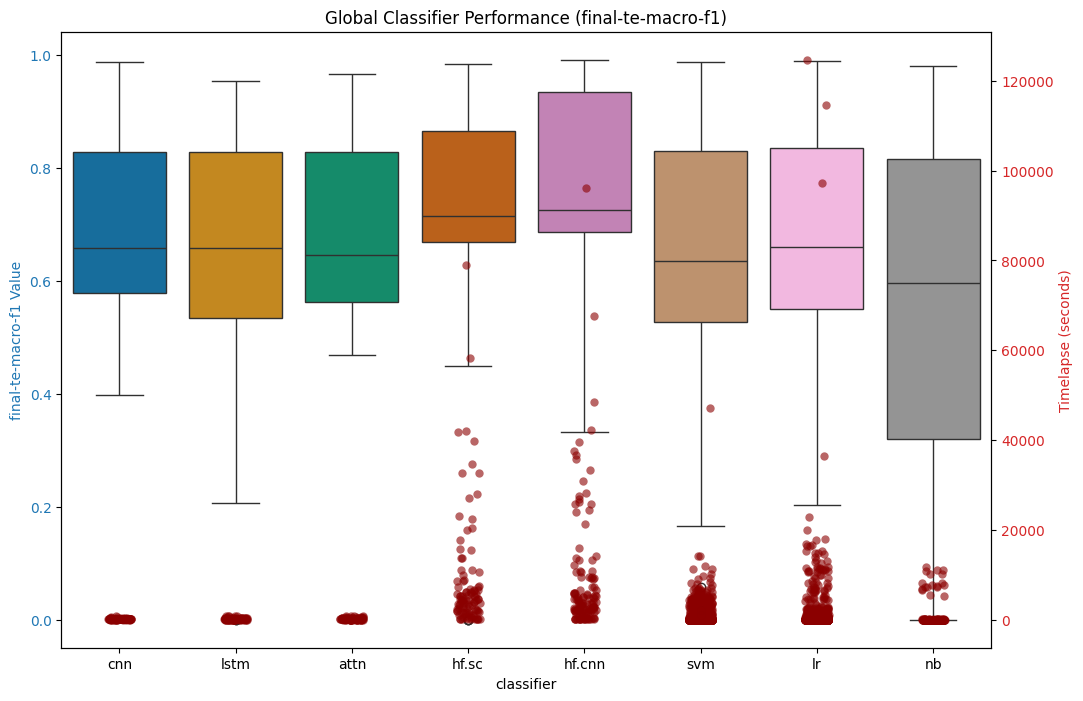
\includegraphics[width=0.8\textwidth, height=7.5cm]{pictures/fig14_global_classifier_perf_macro_f1.png}   
	\caption{\textit{Global Classifier Performance - Macro-F1 Scores}}
	\label{fig14}
\end{figure}

\begin{figure}[h!]
	\centering
	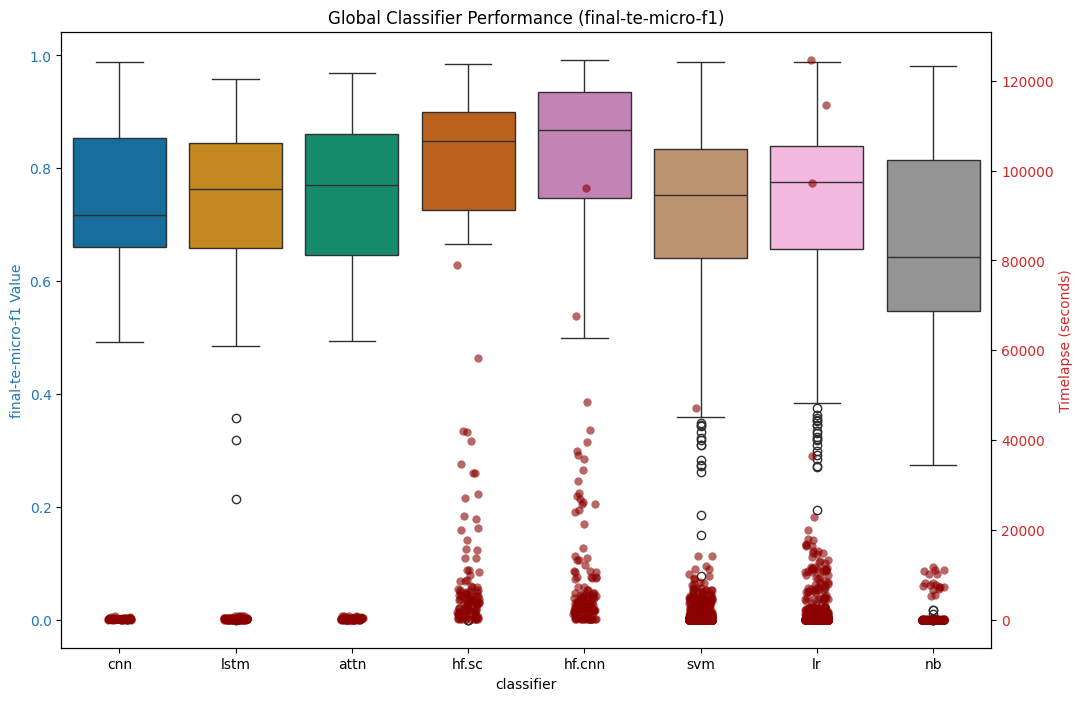
\includegraphics[width=0.8\textwidth, height=7.5cm]{pictures/fig15_global_classifier_perf_micro_f1.png}   
	\caption{\textit{Global Classifier Performance - Micro-F1 Scores}}
	\label{fig15}
\end{figure}

When we look at the detail data for all classifiers across all datasets and language models in Tables \ref{tab:avg_macro_micro_f1} and \ref{tab:summ_avg_macro_micro_f1}, we can see that hf.cnn model is the most performant of all the classifiers, but the static CNN neural model is just .077\% off for average Macro-F1 scores and .09\% off by Micro-F1 scores, while the model training times are less than 2\% of the time it takes to train the hf.cnn models, a 98\% savings in compute effectively.

\begin{table}[h!]
\centering
\scriptsize
\caption{Average Macro-F1 and Micro-F1 Classifier Performance (all datasets and language models)}
\label{tab:avg_macro_micro_f1}
\begin{tabular}{@{}p{1.2cm}p{2.3cm}rrrrr@{}}
\toprule
\textbf{Classifier} & \textbf{Measure} & \textbf{Mean} & \textbf{Median} & \textbf{Std} & \textbf{Count} & \textbf{Time} \\
\midrule
hf.cnn & final-te-macro-f1 & 0.777 & 0.726 & 0.143 & 124 & 9044.06 \\
hf.sc  & final-te-macro-f1 & 0.742 & 0.715 & 0.190 & 101 & 8797.42 \\
cnn    & final-te-macro-f1 & 0.700 & 0.659 & 0.157 & 100 & 164.84 \\
attn   & final-te-macro-f1 & 0.691 & 0.646 & 0.153 & 104 & 197.00 \\
lr     & final-te-macro-f1 & 0.689 & 0.661 & 0.174 & 1539 & 904.00 \\
svm    & final-te-macro-f1 & 0.670 & 0.636 & 0.181 & 1482 & 573.13 \\
lstm   & final-te-macro-f1 & 0.664 & 0.658 & 0.196 & 99 & 186.14 \\
nb     & final-te-macro-f1 & 0.562 & 0.596 & 0.303 & 176 & 870.42 \\
\midrule
hf.cnn & final-te-micro-f1 & 0.849 & 0.867 & 0.100 & 124 & 9044.06 \\
hf.sc  & final-te-micro-f1 & 0.807 & 0.848 & 0.172 & 101 & 8797.42 \\
cnn    & final-te-micro-f1 & 0.759 & 0.716 & 0.126 & 100 & 164.84 \\
lr     & final-te-micro-f1 & 0.755 & 0.775 & 0.137 & 1539 & 904.00 \\
attn   & final-te-micro-f1 & 0.752 & 0.771 & 0.130 & 104 & 197.00 \\
svm    & final-te-micro-f1 & 0.740 & 0.752 & 0.147 & 1482 & 573.13 \\
lstm   & final-te-micro-f1 & 0.727 & 0.763 & 0.177 & 99 & 186.14 \\
nb     & final-te-micro-f1 & 0.644 & 0.642 & 0.241 & 175 & 875.38 \\
\bottomrule
\end{tabular}
\end{table}


\begin{table}[h!]
\centering
\small
\caption{Avg Macro-F1 and Micro-F1 scores by Classifier Type} % <-- Added caption
\label{tab:summ_avg_macro_micro_f1} % <-- Proper label
\begin{tabular}{lrrr} % <-- 'r' = right-align numbers
\toprule
 & \textbf{Macro-F1} & \textbf{Micro-F1} & \textbf{Timelapse (s)} \\
\midrule
avg ML model        & 0.640 & 0.713 &   783.34 \\
avg static neural   & 0.685 & 0.746 &   182.66 \\
avg transformer     & 0.759 & 0.828 &  8920.74 \\
\bottomrule
\end{tabular}
\end{table}

If we look at the performance data by Dataset, as illustrated in Tables \ref{tab:global_classifier_macro_f1_single_label_summary}, \ref{tab:global_classifier_macro_f1_multi_label_summary}, \ref{tab:global_classifier_micro_f1_single_label_summary}, and \ref{tab:global_classifier_micro_f1_multi_label_summary} (in the Appendix), we see the biggest gap between the best transformer models and the next best type of classifier for Macro-F1 values being the largest for the RCV1-V2 dataset, which was the largest dataset we tested with at .185\%, followed by the arxiv dataset at .12\% and then the ohsumed dataset at .078\%. The gap is smaller on the Micro-F1 measure for those datasets at .09\%, .119\% and .062\% respectively. The arxiv gap size being explained possibly by the nature of the underlying data which is not just highly technical but also includes a lot of special symbols and mathematical formulas that transformer models would be better suited at handling than static language models would, or ML classifiers where the data preprocessing would pull much of that noise out of the input data. The glaring exception being the BBC-News dataset, the smallest and most straightforward dataset we tested with, where the CNN classifier performed slightly better than the transformer models, for both Macro-F1 and Micro-F1 measures, but that is due no doubt to its simplicity of format and underlying language being used. 


\begin{table}[h!]
\centering
\scriptsize
\caption{Global Summary Macro-F1 Gap Scores \& Times}
\label{tab:macro_f1_gap_summary}
\begin{tabular}{@{}p{1.3cm} r p{1cm} r p{1cm} p{1cm} p{1cm} p{1cm} p{1.1cm}@{}}
\toprule
\textbf{Dataset} & \textbf{Trans|WE} & \textbf{\%} & \textbf{Trans|ML} & \textbf{\%} & \textbf{Time: Trans|WE} & \textbf{\%} & \textbf{Time: Trans|ML} & \textbf{\%} \\
\midrule
\textbf{20newsgroups}      & 0.018 & 2.60\%  & 0.070 & 10.11\% & 3870.51 & 3441.28\% & 3863.96 & 3257.20\% \\
\textbf{arxiv}             & 0.120 & 16.35\% & 0.107 & 14.67\% & 4377.58 & 3243.87\% & 4317.65 & 2267.81\% \\
\textbf{arxiv\_protoformer}& 0.025 & 3.00\%  & 0.039 & 4.56\%  & 14694.08 & 4138.05\% & 13246.98 & 831.48\% \\
\textbf{bbc-news}          & -0.007 & -0.69\% & 0.004 & 0.38\% & 364.36 & 4843.29\% & 368.81 & 11532.04\% \\
\textbf{imdb}              & 0.046 & 4.91\%  & 0.074 & 7.96\%  & 5514.56 & 5608.59\% & 5474.97 & 4018.99\% \\
\textbf{ohsumed}           & 0.078 & 10.73\% & 0.153 & 21.08\% & 9406.91 & 5897.69\% & 9369.95 & 4803.49\% \\
\textbf{rcv1}              & 0.185 & 26.71\% & 0.199 & 28.63\% & 37169.97 & 5183.25\% & 33191.64 & 804.77\% \\
\textbf{reuters21578}      & 0.044 & 7.38\%  & 0.086 & 14.46\% & 5479.56 & 2828.55\% & 5576.96 & 5492.41\% \\
\midrule
\textbf{AVG:}              & 0.064 & 8.87\%  & 0.091 & 12.73\% & 10109.69 & 4398.07\% & 9426.37 & 4126.02\% \\
\bottomrule
\end{tabular}
\end{table}


\begin{table}[h!]
\centering
\scriptsize
\caption{Global Summary Micro-F1 Gap Scores \& Times}
\label{tab:micro_f1_gap_summary}
\begin{tabular}{@{}p{1.3cm} r p{1cm} r p{1cm} p{1cm} p{1cm} p{1cm} p{1.1cm}@{}}
\toprule
\textbf{Dataset} & \textbf{Trans|WE} & \textbf{\%} & \textbf{Trans|ML} & \textbf{\%} & \textbf{Time: Trans|WE} & \textbf{\%} & \textbf{Time: Trans|ML} & \textbf{\%} \\
\midrule
20newsgroups      & 0.015 & 2.15\%  & 0.070 & 10.05\% & 3870.51 & 3441.28\% & 3863.96 & 3257.20\% \\
arxiv             & 0.119 & 16.05\% & 0.119 & 16.05\% & 4377.58 & 3243.87\% & 4317.65 & 9206.18\% \\
arxiv\_protoformer& 0.027 & 3.15\%  & 0.038 & 4.50\%  & 14694.08 & 4138.05\% & 13246.98 & 831.48\% \\
bbc-news          & -0.007 & -0.68\% & 0.005 & 0.47\% & 364.36 & 4843.29\% & 368.81 & 6173.71\% \\
imdb              & 0.046 & 4.90\%  & 0.074 & 7.96\%  & 5514.56 & 5608.59\% & 5474.97 & 4018.99\% \\
ohsumed           & 0.062 & 8.32\%  & 0.137 & 18.38\% & 9406.91 & 5897.69\% & 9369.95 & 4803.49\% \\
rcv1              & 0.090 & 10.45\% & 0.136 & 15.76\% & 37111.45 & 4799.17\% & 33191.64 & 804.77\% \\
\midrule
reuters21578      & 0.044 & 4.97\%  & 0.087 & 9.83\%  & 5479.56 & 2828.55\% & 5576.96 & 5492.41\% \\
AVG:              & 0.049 & 6.16\%  & 0.083 & 10.38\% & 10102.38 & 4350.06\% & 9426.37 & 4323.53\% \\
\bottomrule
\end{tabular}
\end{table}


However, for the 20newsgroups, arxiv\_protoformer, bbc-news, imdb, and reuters21578 datasets, there exists a static neural model classifier that comes within .05\% on both the Macro-F1 and Micro-F1 measures, indicating that in many cases, these models can compete with the transformer models while greatly reducing computational resource requirements - on average the static neural classifiers took 2.27\% of the amount of time to train, and again this is on 1/4 the number of GPUs or .57\% of the computational resource requirements.

When we look at the overall differences, on average across all the datasets, for the different types of classifiers in comparison with each other, using the best results from each classifier type, we find that on average the best transformer model for a given dataset yields an increase of Macro-F1 score of .064 over the best neural static language model classifier for that dataset, an 8.87\% improvement, and an improvement over the best ML classifier for that dataset, or a 12.73\% improvement. However, to get those better results required - again on average across all the different datasets and using the best model from each classifier type – 10109.69 seconds, or 168.49 minutes, more compute time, a 4398.07\% increase relative to the best static neural classifier for that dataset, and 9426.37 seconds, or 157.11 min, more compute time, a 4126.02\%, increase relative to the best ML classifier for that dataset. 

For the Micro-F1 scores across the different types of classifiers we test with, we see that the best transformer models for each dataset yield an average increase of .049 over the static neural classifiers, and a .083 average increase over the best ML classifiers for the given dataset, a 6.16\% and 10.38\% increase respectively. The performance cost for those improvements were - again on average across all the datasets - 10102.38 seconds (168.37 minutes) over the static neural language model classifiers, and 9426.37 seconds (157.11 minutes) over the best ML classifiers for that dataset, which represent a 4350.06\% and 4323.53\% increase in compute time respectively to achieve said better results.

Furthermore, when we look at the correlation between the (language) model correlation to the timelapse and score metrics, Macro-F1 and Micro-F1, for the largest dataset we tested with, the RCV1-V2 dataset (Figures \ref{fig:fig16} and \ref{fig:fig17})  which is again primarily news data, we can see the transformer models clustered on the top right, indicating that for those last few percentage points for the score requires an exponential amount of computing resources effectively, and you can see that almost all of the transformer models are clustered in that same top-right vicinity indicating that for the most part, they all are achieving similar results and taking a similar amount of compute time. We see a similar pattern for the rest of the datasets as well. 

\begin{figure}[h!]
	\centering
	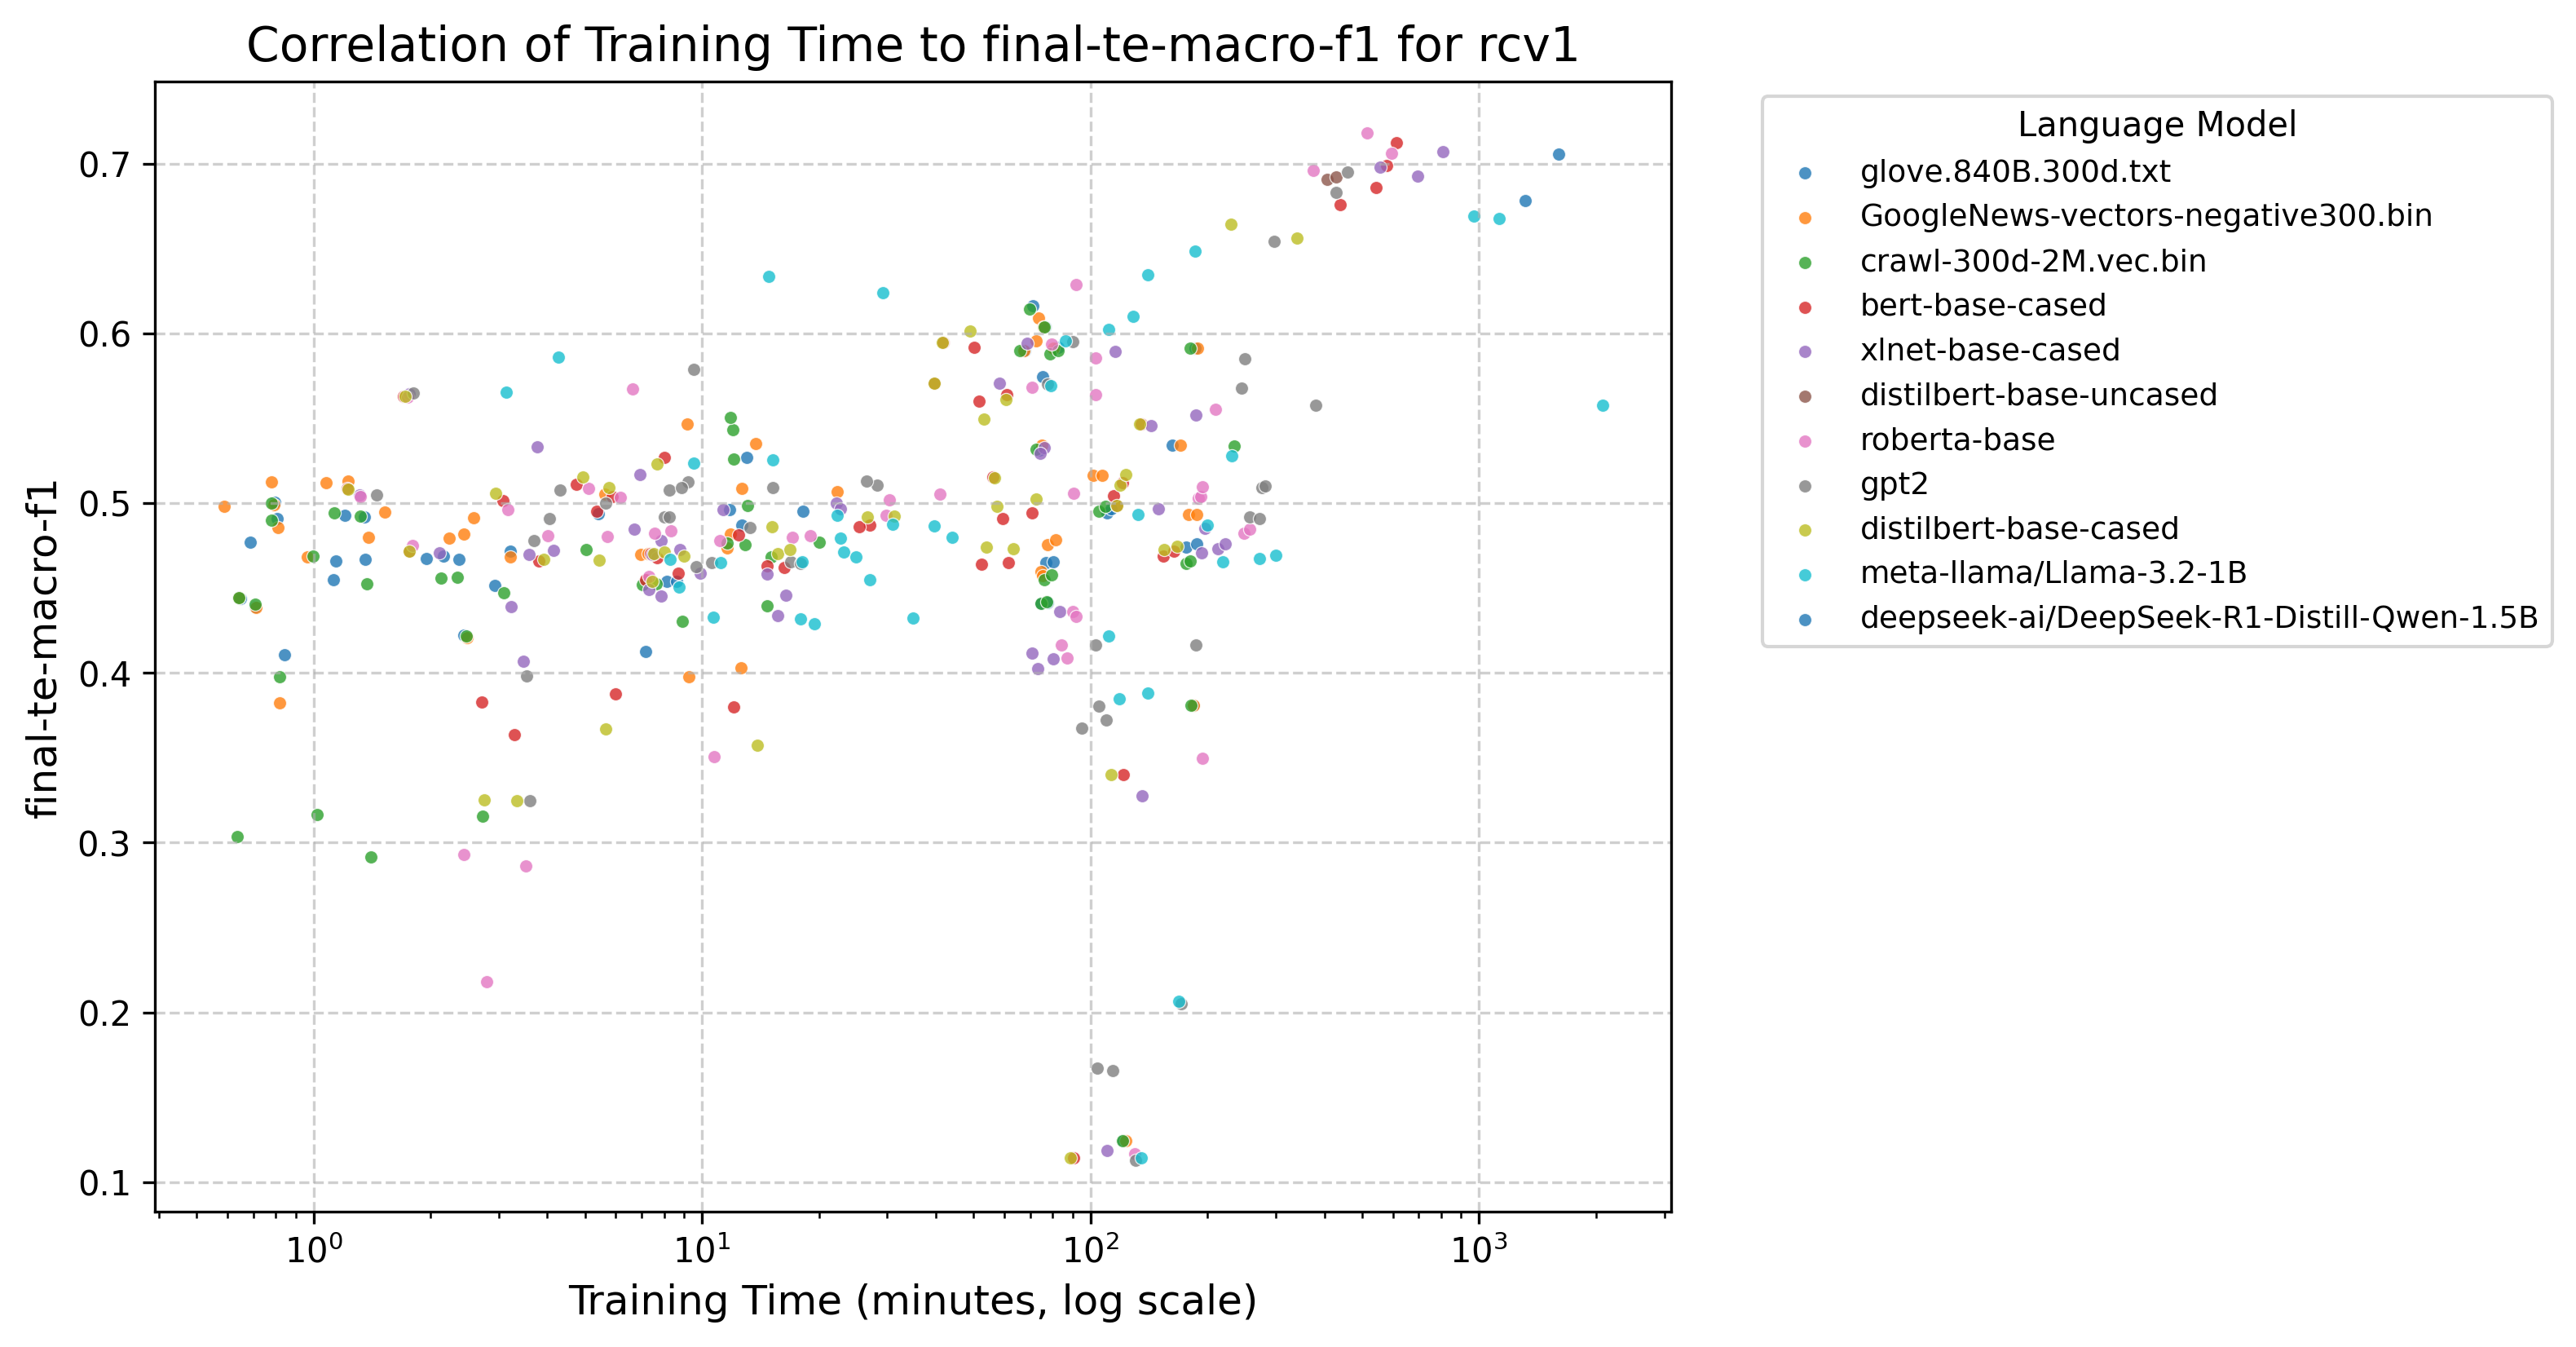
\includegraphics[width=1\textwidth, height=6.5cm]{pictures/fig16_timelapse_model_correlation_rcv1_macro_f1.png}   
	\caption{\textit{Timelapse to Model Correlation, RCV1 dataset Macro-F1 score (logarithmic scale)}}
	\label{fig:fig16}
\end{figure}

\begin{figure}[h!]
	\centering
	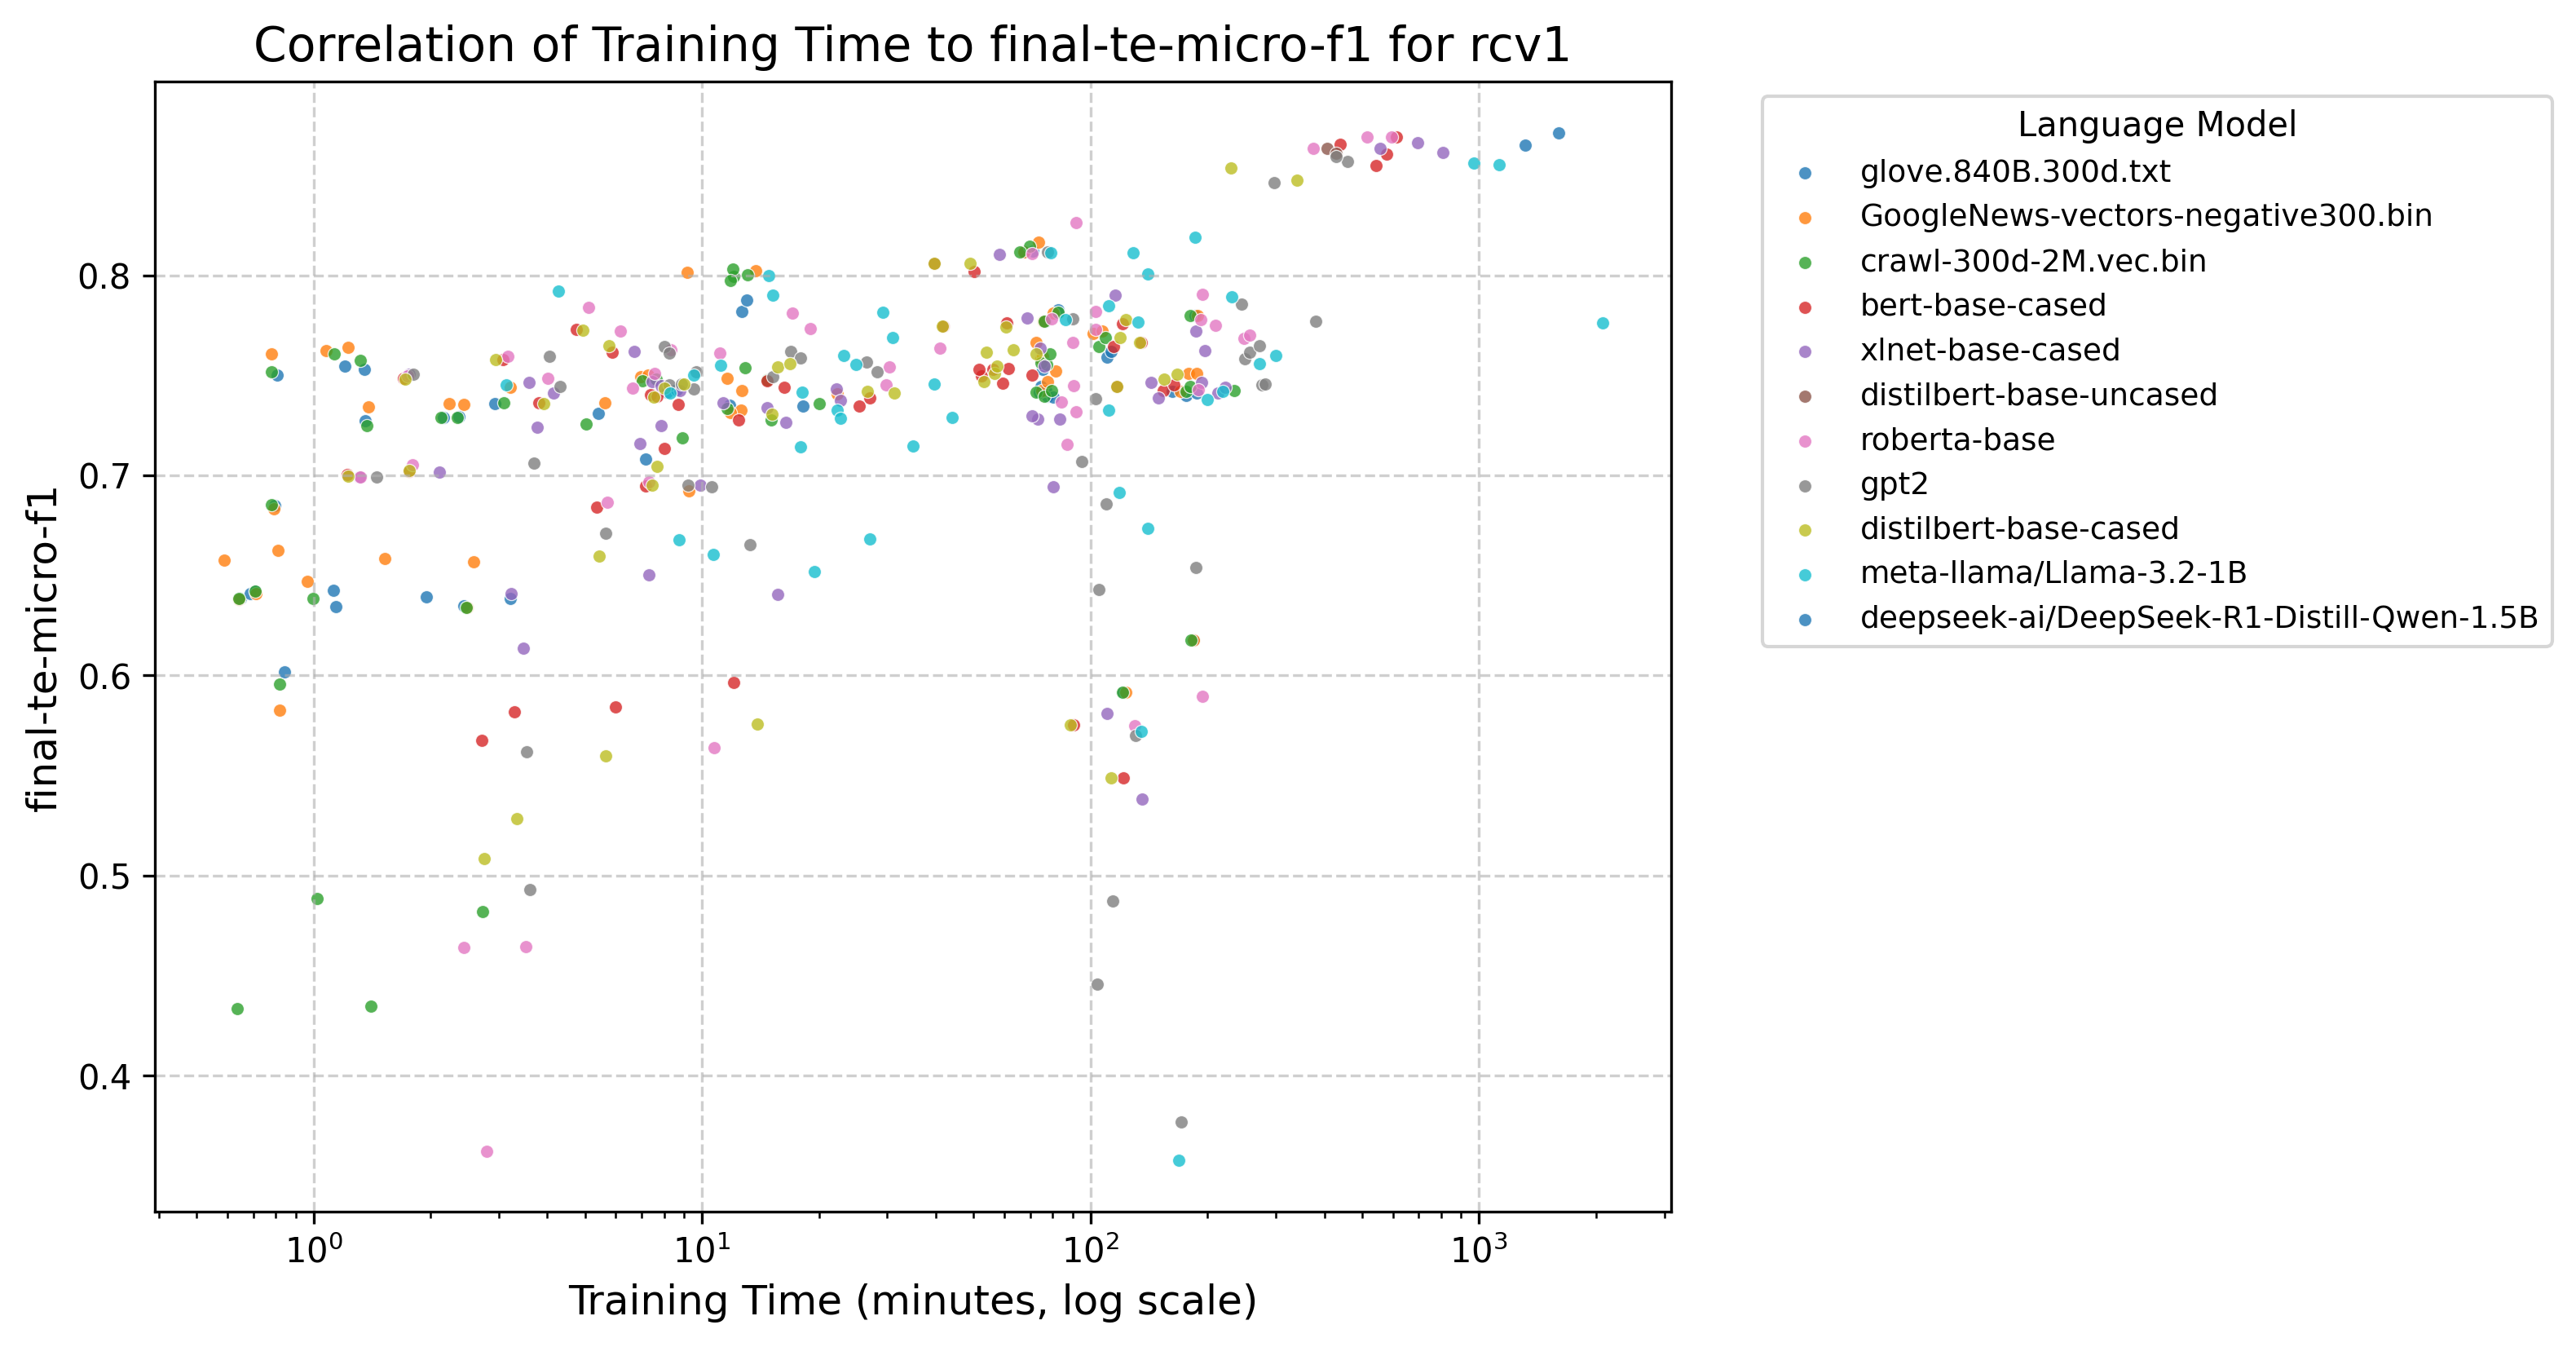
\includegraphics[width=1\textwidth, height=6.5cm]{pictures/fig17_timelapse_model_correlation_rcv1_micro_f1.png}   
	\caption{\textit{Timelapse to Model Correlation, RCV1 dataset Micro-F1 score (logarithmic scale)}}
	\label{fig:fig17}
\end{figure}

A few important points of clarification for the timelapse numbers we report however:
\begin{enumerate}
  \setlength{\itemsep}{2pt} % space between items
  \setlength{\parskip}{0pt} % space between paragraphs
  \setlength{\parsep}{0pt}  % space between item text and paragraph text
  \item the ML classifiers were run with their default options which means that a) the Macro-F1 and Micro-F1 scores are not optimized (they could likely be improved slightly), and b) because they are run without any optimization techniques (like GridSearch Cross Validation for example) their runtimes for the classifier construction are lower than they would be if optimized.
  \item as mentioned previously, the static neural models were run with a single GPU whereas the transformer models ran on 4 GPUs in parallel (same GPU specs for the GPUs), so the timelapse figures for the training times of the transformer models are a factor of (somewhere in the neighborhood of) 4 times their neural counterparts, in terms of computational requirements for classifier training.
  \item The ML classifiers are CPU bound rather than GPU bound so they are not at all an apples-to-apples type of comparison even though we do compare them as such. Having said that however, high end CPUs are much more widely available, and less expensive so it is a reasonable conclusion to suggest that scaling in a CPU bound environment versus a GPU bound environment, at least from a hardware perspective, is, and will remain for the foreseeable future, much less expensive (relatively speaking).
\end{enumerate}

\section{Summary \& Concluding Remarks}

Classifying natural language into predefined categories is a fundamental problem in NLP that has applicability across a wide range of industries, the foundations of which inform other important NLP areas of research such as topic modeling and sentiment analysis, threat and anomaly detection in cyber security, and disease diagnosis in biology, genomics and healthcare. While the problem is very well understood, it nonetheless serves as a very good litmus test for looking at the relative performance characteristics of different types of language models and different types of classifiers with a focus on the underlying (language) representation forms of the different approaches which is the thrust of this work. With this research we have created a robust platform for testing both single-label and multi-label datasets, with language models that range from the static, like Word2Vec, GloVe and FastText, to the dynamic transformer based models from the BERT, RoBERTa, DistilBERT, XLNet, GPT-2, Llama and DeepSeek families, testing them under a variety of hyperparameter conditions, with classical ML classifiers using scikit-learn APIs, as well as DL methods using PyTorch and Hugging Face libraries. Layer Cake produces metrics for all these different configurations and datasets and reports results on model performance in terms of efficacy (Macro-F1, Micro-F1 et al), as well as build and training times (timelapse) and in so doing shed light on the computational requirements of the different approaches that have hitherto been absent from the research literature. By doing so, we hope to help both the research community as well as practitioners in NLP and AI to more easily identify the right model for the right problem, one of the most important design considerations of building out any ML or AI based solution.

In addition to this unique perspective and unique set of findings, we also produce within the context of this work not only the source code for the Layer Cake benchmarking platform itself, but also a rich set of results from Layer Cake, covering a broad spectrum of metrics\footnote{We report macro-f1, micro-f1, precision, recall, accuracy, Jacard-Index and Hamming loss metrics for each test run.} that is readily available for further analysis, contributing to the research community a cross-platform, extensible, benchmarking platform that supports a variety of language models, classifiers and datasets that can be extended for further insights into this field of research, i.e. text classification, or even extended to support other NLP problems like sentiment classification, topic modeling or even Natural Language Understanding (NLU) benchmarking if need be.\footnote{Layer Cake supports Mac MPS GPU architectures as well as Ubuntu Linux GPU architectures with the exception being the DeepSeek models which are not supported (yet) on MacOS. Source available on GitHub at Source code for Layer Cake available at https://github.com/pworth1971/layer-cake.} 

Furthermore, while ML classifiers typically depend on text vectorization techniques for language representation, we show that LSA as well as various forms of embedding representations also perform competitively in an ML classifier setting, both reproducing and expanding (baseline) results from \cite{moreo2021}, adding both fastText and Word2Vec language models into the analysis for comparison purposes. The Deep Learning classifiers we test with on the other hand, require fundamentally different forms of language representation than their ML counterparts, coming in word, subword and token based variants with the token based variants requiring specific transformer based models (Hugging Face). These DL approaches, as expected, show strong performance in our tests, with the static DL models (for word and subword embeddings) proving to be computationally efficient, albeit somewhat less effective than the transformer based DL models. The latter models however, come with some constraints, for example the inability to work with externally computed embeddings such as TCEs, illustrating both some of the architectural drawbacks of modern transformer based classifiers as well as their inherent effectiveness, without TCEs, as it relates to the problem at hand

. Also with respect to the ML testing and analysis part of this research, we include a broad spectrum of language representation forms into the models to test their relative efficacy, an aspect of model design that is oft overlooked in the text classification and NLP research literature, especially given that LLMs presume a fixed structure of language representation that is necessary for the models to work whereas the ML models have more flexibility with how the model is prepared with data, i.e. how the text is represented.\footnote{With LLMs, and in fact with almost all neural models in NLP, the underling (natural) language is converted into a fixed size (max\_width) sequence of token indices where each token is represented by a vector of real numbers of a size fixed by the language model (aka hidden\_size) that is the result of the pretraining of that language model against a fixed pretraining dataset - i.e. what are known as embeddings but which are extensions of Vector Space Models which have been around since the 1970s. Each LLM creates these embeddings by defining the underling vector space dimensions (as a form of feature reduction from the total dictionary size of the pretrained corpus) and then learning the embeddings for each token using the language model type and variant specific (neural) architecture and algorithm (loss function, etc.).} 

Also, in the testing of different neural classifier variants to support both static language models as well as transformer, context aware models, we discovered a significant difference in the flexibility of the different neural architectural models, with the transformer embedding layer being tightly coupled with its computational logic (as one might expect perhaps), which significantly limits the ability to optimize the model – like for example using feature, or dictionary size, reduction techniques as we do for the other classifiers. This constraint, limits how and where in model training one can add pretrained embedding structures that are extra-model or are trained outside the transformer language model context that we are using for the task at hand.  In our testing for example, we could not find an approach where the integration of Token-Class Embeddings, or TCEs (the transformer variant of WCEs), actually increased the effectiveness of the model, in fact we found the opposite, that adding these TCEs with the context-aware embeddings during training - no matter how we added them or how we normalized the underlying embedding dimensions - actually made the model less effective. What we also find, is that Word-Class Embeddings, which have been shown to improve the performance of text classification models in both ML classifier context as well as static embedding neural models, are not at all effective in a transformer, context-aware embedding environment. This is in all likelihood due to a combination of a) the already granular, context-aware nature of the transformer models which include this type of word/token to class type information, and b) the transformer-based models are designed to be self-contained and are not set up to be augmented with additional embedding information that comes from outside the model. This is of course another important factor that should be considered when determining which type of language model is optimal for a given problem, whether or not it is of value to include embeddings that are computed outside of the model to boost performance.

What we do with this research is to ground the conversation about LLM performance in a computational context so that actual performance gains can be understood relative to the computational cost necessary to achieve such gains. And while most certainly we can expect continued investment in GPU architecture to help solve for this computational gap, if we may coin a phrase here, nonetheless the cost of closing this gap at the present time, given the numbers we report in this work, remains a quite expensive proposition. At present, to procure environments that leverage a single NVIDIA H100 which sits at the forefront of AI and LLM training GPU technology right now, a chip with 80GB of RAM which is optimized for LLM training specifically going for anywhere between \$2 and \$3 an hour.\footnote{Reflects current list hourly prices available from CoreWeave, AWS, Lambda and JarvisLabs as of 04/12/2025.} These chips have 80GB of memory and while list at around \$25,000 per chip, can go for more depending upon availability. In contrast, an Apple MacBook with an M3 chip with 128GB of RAM, which is available for both the MPS (GPU) and CPU chips on that system that are available costs anywhere between \$5000 and \$6000 depending upon configuration.\footnote{Source: Amazon.} While this is not necessarily a straight apples to apples comparison, it nonetheless sheds light on just how much more computationally expensive these LLMs are to use in the event that there exist more straightforward, and less computationally intensive, options for the same solve. Our findings show that yes, transformer models do in fact perform better on average than their static language models counterparts, 8.87\% better on average than static embedding DL classifiers from a Macro-F1 score perspective, and better than classical ML classifiers by 12.73\%, but these gains come with significant additional computational requirements - 4398.07\% and 4126.02\% respectively. Similarly, with respect to Micro-F1 score, we see the LLMs outperform the static language model DL methods by 6.16\%, and by 10.38\% versus the ML classifiers, but those gains coming at a compute cost of 4350.06\% over the static neural language model classifiers, and 4323.53\% increase in compute time for the training of the ML classifiers. And these numbers do not take into account that we were using 4x the number of GPUs to train the transformer models, albeit using the less performant PyTorch form of model parallelism called DataParallel (DP).


This kind of research is absolutely essential for the AI and ML research and development community so that practical decisions can be made about how and when LLMs should be used in real-world contexts where cost, and time, are important ingredients for successful outcomes. In short, in this work we look to answer the question, again within the context of text classification specifically but with broader implications on how these LLMs are being used to solve NLP problems more generally, what kind of performance improvement can we expect to gain by using these LLMs and at what (computational) cost? Our findings here show that, consistent with past research on LLM performance in NLP, the best performing models are in fact LLMs, but a) they cost significantly more time and money to train and b) in almost all cases there exists a classical ML, CPU bound alternative that performs almost as well as best transformer models for that particular dataset. 


\subsection{Areas of Further Research }

While the testing we've done with Layer Cake covers a broad spectrum of classifiers and language model forms, we nonetheless limit the study to Euclidean spatial geometry, i.e. all of the language representation forms we work with are constructed in Euclidean spaces. However, there is a lot of promising research that has been done with hyperbolic geometry \cite{tifrea} \cite{leimeister2019skip} \cite{valentino} and it would be very interesting to see how these embedding forms performed relatively speaking, or to see if using these embeddings that are trained in hyperbolic spaces, which lend themselves to a more hierarchical structure, could be used in conjunction with some of the other language representation forms we test with (like we do with WCEs) and what kind of effect performance wise that had on the models.

From a performance standpoint, it would also be interesting to see what the effect might be of using different parallelism approaches to transformer model training to see what kind of performance effects they had on model training times, effectively extending Layer Cake to support such analysis. In our case, we used the default DataParallel (DP) approach which comes built into the Hugging Face APIs but the Distributed Data Parallel (DDP) PyTorch capabilities are supposed to surpass those of the more straightforward DP form of parallelism so it would be interesting to see what this difference was performance wise in terms of model training. Using DPP would also allow the testing of larger LLMs, LLMs that could be spread across multiple GPUs - models that could not be included in this study due to single GPU memory constraints that prevent the use of larger models in a DP type of setup. 

Also from a performance perspective, it would be informative to further evaluate various parameterization tuning methods, for example as described \cite{lee} or in the more comprehensive look at parameter efficient fine-tuning methods (PEFT) from 2023 \cite{articleding}. In our tests, we did not find the language models, specifically the transformer-based classifiers, to be performant when freezing only a certain number of layers, forcing a re-training of all of the model layers for our fine-tuning experiments which is the most computationally expensive approach to fine-tuning (at least from a Layer freezing perspective). This is a somewhat unexpected result so it would be valuable to evaluate various PEFT approaches within the context of the text classification problem as defined in Layer Cake for transformer-based classifiers to see what is optimal. 

From a language representation perspective, in particular with respect to the Deep Learning approaches we cover with Layer Cake, it would be interesting to see if we could combine vectorization based approaches with the standard token indexing approaches to the model, particularly within the context of classification problems as that would give us an opportunity perhaps, like with tf-idf vectorization, to weight the different tokens alongside the attention based masking that the transformer models are known for. This has been shown to be an effective approach for certain NLP problems, like sentiment analysis, as exemplified in \cite{liang2022research} \cite{zhao2022research} \cite{kamyab2021attention}.

Further research in these areas would no doubt be of value to both the research and practitioner community around language model efficacy within NLP, in particular in light of the fact that we can expect that much research over the coming years will be focused both on the performance and power of LLMs with respect to problem solving capabilities and other deep reasoning functionality, as well as optimization techniques related to minimizing the computational and system requirements to both build and tune LLMs as they are pre-trained with more and more data and get larger and larger over time.

\bibliographystyle{unsrt}

\bibliography{Layer-Cake-bib-07212025}


\section{Appendix: Global Classifier Performance Data}


\begin{table}[h!]
\centering
\tiny
\caption{Global Macro-F1 Classifier Performance Summary (single-label datasets)}
\label{tab:global_classifier_macro_f1_single_label_summary}
\resizebox{\textwidth}{!}{%
\begin{tabular}{@{}p{2cm}p{1.2cm}rrrrr@{}}
\toprule
\textbf{Dataset} & \textbf{Classifier} & \textbf{Mean} & \textbf{Median} & \textbf{Std} & \textbf{Count} & \textbf{Time} \\
\midrule
\textbf{20newsgroups} & hf.cnn & 0.690 & 0.688 & 0.009 & 13 & 3986.35 \\
 & hf.sc & 0.683 & 0.684 & 0.012 & 13 & 3843.29 \\
 & cnn & 0.672 & 0.674 & 0.014 & 12 & 115.84 \\
 & attn & 0.646 & 0.642 & 0.021 & 12 & 54.03 \\
 & lstm & 0.640 & 0.642 & 0.030 & 12 & 56.35 \\
 & lr & 0.620 & 0.641 & 0.075 & 186 & 122.39 \\
 & svm & 0.590 & 0.625 & 0.093 & 186 & 60.39 \\
 & nb & 0.586 & 0.596 & 0.056 & 20 & 11.70 \\
\midrule
\textbf{arxiv\_protoformer} & hf.cnn & 0.848 & 0.847 & 0.006 & 13 & 15057.97 \\
 & hf.sc & 0.847 & 0.847 & 0.008 & 13 & 13097.29 \\
 & attn & 0.823 & 0.824 & 0.007 & 12 & 363.89 \\
 & lstm & 0.822 & 0.824 & 0.007 & 11 & 329.44 \\
 & lr & 0.810 & 0.821 & 0.040 & 244 & 1810.99 \\
 & nb & 0.808 & 0.808 & 0.008 & 38 & 49.06 \\
 & svm & 0.806 & 0.821 & 0.034 & 187 & 1049.55 \\
 & cnn & 0.804 & 0.807 & 0.019 & 12 & 276.43 \\
\midrule
\textbf{bbc-news} & cnn & 0.979 & 0.982 & 0.009 & 12 & 7.68 \\
 & hf.cnn & 0.973 & 0.972 & 0.010 & 25 & 372.04 \\
 & hf.sc & 0.972 & 0.972 & 0.008 & 13 & 338.51 \\
 & lr & 0.969 & 0.980 & 0.033 & 186 & 3.23 \\
 & nb & 0.968 & 0.975 & 0.014 & 20 & 0.09 \\
 & svm & 0.948 & 0.974 & 0.099 & 186 & 3.18 \\
 & attn & 0.947 & 0.944 & 0.011 & 12 & 7.91 \\
 & lstm & 0.931 & 0.927 & 0.015 & 12 & 7.34 \\
\midrule
\textbf{imdb} & hf.sc & 0.929 & 0.934 & 0.026 & 13 & 5614.67 \\
 & hf.cnn & 0.889 & 0.935 & 0.167 & 13 & 5343.42 \\
 & attn & 0.883 & 0.884 & 0.008 & 12 & 100.11 \\
 & cnn & 0.870 & 0.869 & 0.012 & 12 & 173.42 \\
 & lstm & 0.867 & 0.870 & 0.018 & 12 & 126.45 \\
 & lr & 0.855 & 0.857 & 0.036 & 190 & 139.70 \\
 & svm & 0.843 & 0.849 & 0.058 & 190 & 94.81 \\
 & nb & 0.821 & 0.827 & 0.018 & 20 & 4.90 \\
\bottomrule
\end{tabular}%
}
\end{table}

\begin{table}[h!]
\centering
\tiny
\caption{Global Macro-F1 Classifier Performance Summary (multi-label datasets)}
\label{tab:global_classifier_macro_f1_multi_label_summary}
\resizebox{\textwidth}{!}{%
\begin{tabular}{@{}p{2cm}p{1.2cm}rrrrr@{}}
\toprule
\textbf{Dataset} & \textbf{Classifier} & \textbf{Mean} & \textbf{Median} & \textbf{Std} & \textbf{Count} & \textbf{Time} \\
\midrule
\textbf{arxiv} & hf.cnn & 0.731 & 0.726 & 0.029 & 13 & 4516.82 \\
 & lr & 0.624 & 0.652 & 0.098 & 186 & 199.17 \\
 & svm & 0.611 & 0.638 & 0.108 & 186 & 82.80 \\
 & cnn & 0.595 & 0.595 & 0.052 & 24 & 139.24 \\
 & attn & 0.579 & 0.580 & 0.060 & 24 & 152.10 \\
 & hf.sc & 0.547 & 0.681 & 0.314 & 13 & 6640.57 \\
 & lstm & 0.499 & 0.568 & 0.200 & 23 & 159.15 \\
 & nb & 0.234 & 0.226 & 0.236 & 20 & 9.24 \\
\midrule
\textbf{ohsumed} & hf.cnn & 0.726 & 0.724 & 0.011 & 13 & 9569.17 \\
 & hf.sc & 0.715 & 0.712 & 0.021 & 13 & 8848.25 \\
 & lstm & 0.649 & 0.654 & 0.029 & 12 & 162.25 \\
 & attn & 0.643 & 0.648 & 0.029 & 12 & 188.86 \\
 & cnn & 0.634 & 0.649 & 0.036 & 12 & 204.21 \\
 & lr & 0.573 & 0.603 & 0.089 & 190 & 199.21 \\
 & svm & 0.567 & 0.585 & 0.084 & 190 & 635.01 \\
 & nb & 0.309 & 0.287 & 0.175 & 20 & 13.83 \\
\midrule
\textbf{rcv1} & hf.cnn & 0.694 & 0.695 & 0.017 & 13 & 37901.20 \\
 & hf.sc & 0.679 & 0.682 & 0.018 & 8 & 38358.23 \\
 & attn & 0.508 & 0.504 & 0.037 & 8 & 731.22 \\
 & lr & 0.495 & 0.492 & 0.066 & 171 & 4709.55 \\
 & svm & 0.479 & 0.479 & 0.070 & 171 & 2726.32 \\
 & lstm & 0.478 & 0.487 & 0.056 & 5 & 789.74 \\
 & cnn & 0.435 & 0.421 & 0.045 & 4 & 575.69 \\
 & nb & 0.221 & 0.165 & 0.116 & 18 & 8349.90 \\
\midrule
\textbf{reuters21578} & hf.cnn & 0.596 & 0.606 & 0.044 & 21 & 5680.39 \\
 & hf.sc & 0.565 & 0.547 & 0.074 & 15 & 5513.30 \\
 & attn & 0.552 & 0.553 & 0.030 & 12 & 200.82 \\
 & cnn & 0.536 & 0.533 & 0.028 & 12 & 125.66 \\
 & lr & 0.510 & 0.526 & 0.068 & 186 & 103.42 \\
 & svm & 0.498 & 0.513 & 0.064 & 186 & 113.00 \\
 & lstm & 0.481 & 0.484 & 0.039 & 12 & 247.16 \\
 & nb & 0.290 & 0.256 & 0.094 & 20 & 11.78 \\
\bottomrule
\end{tabular}%
}
\end{table}


\begin{table}[h!]
\centering
\tiny
\caption{Global Micro-F1 Classifier Performance Summary (single-label datasets)}
\label{tab:global_classifier_micro_f1_single_label_summary}
\resizebox{\textwidth}{!}{%
\begin{tabular}{@{}p{2cm}p{1.2cm}rrrrr@{}}
\toprule
\textbf{Dataset} & \textbf{Classifier} & \textbf{Mean} & \textbf{Median} & \textbf{Std} & \textbf{Count} & \textbf{Time} \\
\midrule
\textbf{20newsgroups} & hf.cnn & 0.699 & 0.698 & 0.010 & 13 & 3986.35 \\
 & hf.sc & 0.693 & 0.695 & 0.010 & 13 & 3843.29 \\
 & cnn & 0.684 & 0.686 & 0.014 & 12 & 115.84 \\
 & attn & 0.655 & 0.651 & 0.020 & 12 & 54.03 \\
 & lstm & 0.650 & 0.655 & 0.029 & 12 & 56.35 \\
 & lr & 0.629 & 0.651 & 0.076 & 186 & 122.39 \\
 & nb & 0.610 & 0.624 & 0.065 & 20 & 11.70 \\
 & svm & 0.596 & 0.631 & 0.097 & 186 & 60.39 \\
\midrule
\textbf{arxiv\_protoformer} & hf.cnn & 0.849 & 0.848 & 0.006 & 13 & 15057.97 \\
 & hf.sc & 0.846 & 0.848 & 0.008 & 13 & 13097.29 \\
 & attn & 0.822 & 0.823 & 0.007 & 12 & 363.89 \\
 & lstm & 0.821 & 0.824 & 0.007 & 11 & 329.44 \\
 & lr & 0.810 & 0.821 & 0.039 & 244 & 1810.99 \\
 & nb & 0.809 & 0.810 & 0.009 & 38 & 49.06 \\
 & svm & 0.807 & 0.821 & 0.034 & 187 & 1049.55 \\
 & cnn & 0.803 & 0.807 & 0.018 & 12 & 276.43 \\
\midrule
\textbf{bbc-news} & cnn & 0.981 & 0.983 & 0.009 & 12 & 7.68 \\
 & hf.cnn & 0.974 & 0.973 & 0.009 & 25 & 372.04 \\
 & hf.sc & 0.973 & 0.973 & 0.007 & 13 & 338.51 \\
 & lr & 0.969 & 0.981 & 0.033 & 186 & 3.23 \\
 & nb & 0.968 & 0.975 & 0.014 & 20 & 0.09 \\
 & attn & 0.951 & 0.946 & 0.010 & 12 & 7.91 \\
 & svm & 0.950 & 0.973 & 0.093 & 186 & 3.18 \\
 & lstm & 0.935 & 0.929 & 0.014 & 12 & 7.34 \\
\midrule
\textbf{imdb} & hf.sc & 0.929 & 0.934 & 0.026 & 13 & 5614.67 \\
 & hf.cnn & 0.902 & 0.935 & 0.121 & 13 & 5343.42 \\
 & attn & 0.883 & 0.884 & 0.008 & 12 & 100.11 \\
 & cnn & 0.870 & 0.869 & 0.012 & 12 & 173.42 \\
 & lstm & 0.867 & 0.870 & 0.018 & 12 & 126.45 \\
 & lr & 0.855 & 0.857 & 0.036 & 190 & 139.70 \\
 & svm & 0.845 & 0.849 & 0.049 & 190 & 94.81 \\
 & nb & 0.820 & 0.827 & 0.018 & 19 & 5.10 \\
\bottomrule
\end{tabular}%
}
\end{table}


\begin{table}[h!]
\centering
\tiny
\caption{Global Micro-F1 Classifier Performance Summary (multi-label datasets)}
\label{tab:global_classifier_micro_f1_multi_label_summary}
\resizebox{\textwidth}{!}{%
\begin{tabular}{@{}p{2cm}p{1.2cm}rrrrr@{}}
\toprule
\textbf{Dataset} & \textbf{Classifier} & \textbf{Mean} & \textbf{Median} & \textbf{Std} & \textbf{Count} & \textbf{Time} \\
\midrule
\textbf{arxiv} & hf.cnn & 0.739 & 0.733 & 0.028 & 13 & 4516.82 \\
 & lr & 0.620 & 0.656 & 0.107 & 186 & 199.17 \\
 & cnn & 0.615 & 0.616 & 0.047 & 24 & 139.24 \\
 & svm & 0.611 & 0.643 & 0.115 & 186 & 82.80 \\
 & attn & 0.591 & 0.596 & 0.059 & 24 & 152.10 \\
 & hf.sc & 0.553 & 0.685 & 0.318 & 13 & 6640.57 \\
 & lstm & 0.510 & 0.585 & 0.203 & 23 & 159.15 \\
 & nb & 0.221 & 0.213 & 0.222 & 20 & 9.24 \\
\midrule
\textbf{ohsumed} & hf.cnn & 0.746 & 0.748 & 0.009 & 13 & 9569.17 \\
 & hf.sc & 0.739 & 0.736 & 0.015 & 13 & 8848.25 \\
 & lstm & 0.684 & 0.687 & 0.020 & 12 & 162.25 \\
 & attn & 0.675 & 0.677 & 0.020 & 12 & 188.86 \\
 & cnn & 0.673 & 0.677 & 0.028 & 12 & 204.21 \\
 & lr & 0.609 & 0.633 & 0.080 & 190 & 199.21 \\
 & svm & 0.602 & 0.616 & 0.074 & 190 & 635.01 \\
 & nb & 0.422 & 0.391 & 0.110 & 20 & 13.83 \\
\midrule
\textbf{rcv1} & hf.cnn & 0.863 & 0.863 & 0.006 & 13 & 37901.20 \\
 & hf.sc & 0.857 & 0.858 & 0.008 & 8 & 38358.23 \\
 & lstm & 0.773 & 0.782 & 0.031 & 5 & 789.74 \\
 & attn & 0.769 & 0.771 & 0.032 & 8 & 731.22 \\
 & cnn & 0.730 & 0.713 & 0.048 & 4 & 575.69 \\
 & lr & 0.727 & 0.750 & 0.073 & 171 & 4709.55 \\
 & svm & 0.723 & 0.742 & 0.067 & 171 & 2726.32 \\
 & nb & 0.558 & 0.575 & 0.073 & 18 & 8349.90 \\
\midrule
\textbf{reuters21578} & hf.cnn & 0.886 & 0.887 & 0.008 & 21 & 5680.39 \\
 & hf.sc & 0.876 & 0.876 & 0.015 & 15 & 5513.30 \\
 & attn & 0.842 & 0.838 & 0.017 & 12 & 200.82 \\
 & cnn & 0.840 & 0.838 & 0.010 & 12 & 125.66 \\
 & lstm & 0.813 & 0.816 & 0.029 & 12 & 247.16 \\
 & lr & 0.799 & 0.820 & 0.065 & 186 & 103.42 \\
 & svm & 0.787 & 0.807 & 0.089 & 186 & 113.00 \\
 & nb & 0.591 & 0.629 & 0.108 & 20 & 11.78 \\
\bottomrule
\end{tabular}%
}
\end{table}

\end{document}
